\documentclass[12pt, hidelinks]{book}

\usepackage{hyperref}
\def\chapterautorefname{Chapter}
\def\sectionautorefname{Section}
\def\subsectionautorefname{Section}
\def\subsubsectionautorefname{Section}

\usepackage{algorithm}
\usepackage{algpseudocode}
\algrenewcommand\algorithmicrequire{\textbf{Input:}}
\algrenewcommand\algorithmicensure{\textbf{Output:}}
\algnewcommand\Not{\textbf{not} }
\newcommand{\algorithmautorefname}{Algorithm} % autoref

\usepackage{adjustbox}
\usepackage[headings]{fullpage}
\usepackage{xargs}
\usepackage{xspace}
\usepackage[doublespacing]{setspace}

\usepackage{microtype}
\usepackage[T1]{fontenc}

\usepackage{wrapfig}
\usepackage[font={sf}]{caption}
\usepackage[subrefformat=parens]{subcaption}

\usepackage{multirow}

\usepackage{xcolor}
\usepackage{graphicx}
\graphicspath{{_build/}{figures/}}

\usepackage{amsmath}
\usepackage{amssymb}
\newtheorem{definition}{Definition}[chapter]
\newtheorem{theorem}{Theorem}[chapter]
\newtheorem{proof}{Proof}[chapter]

\setlength{\marginparwidth}{2cm}
\usepackage[textsize=tiny]{todonotes}

\usepackage{libertine}
\usepackage[libertine]{newtxmath}
\usepackage[scaled=.85]{DejaVuSansMono}

\usepackage{listings}
\lstset{
  columns=fullflexible,
  keepspaces=true,
  showstringspaces=false,
  stringstyle=\slshape\color{green!40!black},
  basicstyle=\ttfamily\small,
  language=Python,
  morekeywords={*, self},
  commentstyle=\slshape\color{black!60},
  tabsize=2,
}

\lstdefinelanguage{Rust}{
  sensitive,
  morecomment=[l]{//},
  morecomment=[s]{/*}{*/},
  moredelim=[s][{\itshape\color[rgb]{0,0,0.75}}]{\#[}{]},
  morestring=[b]{"},
  alsodigit={},
  alsoother={},
  alsoletter={!},
  % keywords
  otherkeywords={=>},
  morekeywords={break, continue, else, for, if, in, loop, match, return, while},
  morekeywords={as, const, let, move, mut, ref, static, unsafe},
  morekeywords={dyn, enum, fn, impl, Self, self, struct, trait, type, use, where},
  morekeywords={crate, extern, mod, pub, super},
  morekeywords={abstract, alignof, become, box, do, final, macro,
    offsetof, override, priv, proc, pure, sizeof, typeof, unsized, virtual, yield},
  % traits
  morekeywords=[2]{Send},
  % types
  morekeywords=[3]{bool, char, f32, f64, i8, i16, i32, i64, isize, str, u8, u16, u32, u64, unit, usize, i128, u128},
}%

\def\mytitle{Something about hardware}
\def\myauthor{Gus Henry Smith}
\def\year{2024}

\title{\mytitle}
\author{\myauthor}

\newcommand\thesisstmt{%
something something
}

\newcommand\Thesisstmt{\expandafter\MakeUppercase \thesisstmt}

% General thesis imports
\usepackage{mdframed}
\usepackage{glossaries}

% Bold the first occurrence of a glossary word
\DeclareRobustCommand{\glossfirstformat}[1]{\textit{#1}}
\renewcommand*{\glsdisplayfirst}[4]{\glossfirstformat{#1#4}}
\usepackage[normalem]{ulem}
\renewcommand*{\glstextformat}[1]{\color{lightgray}{\dotuline{\color{black} #1}}}


% \makeglossaries
\makenoidxglossaries

% NOTE: use \glstext and not \gls in this file.
% This prevents the glossary from thinking that uses of these words in the glossary are the first occurrence in text. We'd rather those first occurrences happen e.g. in the intro.

\newglossaryentry{compiler}
{
    name=compiler,
    description={
A tool which converts between representations.
    }
}


\newglossaryentry{target}
{
    name=target,
    description={
The platform which a \glstext{compiler} generates code for.
    }
}

\newglossaryentry{compilerbackend}
{
    name=compiler backend,
    description={
The portion of a \glstext{compiler} that concerns the \glstext{target},
  e.g., target-specific optimizations and code generation.
    }
}

\newglossaryentry{validation}
{
    name=validation,
    description={
The process of sanity-checking a program or hardware design using a
  limited, finite set
  of inputs, and judging the correctness 
  of the outputs.
Also referred to as \textit{testing.}
Validation should specifically be distinguished from
  \glstext{verification}.
Confusingly, 
  in the world of hardware design,
  validation is often referred to as
  verification,
  while verification (by our definition)
  is referred to as \textit{formal} verification.
    }
}

\newglossaryentry{verification}
{
    name=verification,
    description={
The process of mathematically proving correctness
  about a program or hardware design.
While the proofs of correctness themselves
  can have limitations,
  verification is generally more thorough
  than \glstext{validation} or \textit{testing.}
In the world of hardware design,
  ``verification''
  generally refers to what we call validation or testing,
  while ``formal verification''
  refers to our verification.
    }
}

\newglossaryentry{hardwaresynthesis}
{
    name={hardware synthesis},
    description={
Another term for hardware compilation.
The process of converting a hardware design
  captured in a high-level language
  to a low-level target implementation,
  for example,
  a netlist which can be programmed onto an FPGA
  or a geometry file to be made into an ASIC.
  \hl{define the terms in here}
    }
}

% Note: this is a nice hack from
% https://tex.stackexchange.com/questions/8946/how-to-combine-acronym-and-glossary
% which gives acronym-like behavior but
% still allows for a definition.
\newglossaryentry{dsl}
{
    name={DSL},
    first={domain-specific language (DSL)},
    description={
A language designed for a custom purpose \hl{fill out}
    }
}

\newglossaryentry{mlkernel}
{
    name={machine learning kernel},
    description={
A core subroutine used within many machine learning workloads---for example,
  matrix multiplication.
Machine learning kernels are often highly optimized,
  often by building custom hardware to implement
  them efficiently.
    }
}

% Glenside imports
\usepackage{soul}
\usepackage{ragged2e}
\usepackage{caption}
\usepackage{subcaption}
\usepackage[utf8]{inputenc}
%\usepackage{syntax} % for grammar
\usepackage{tabularx}
\usepackage{listings}
\usepackage{amsmath}
\usepackage{xspace}
%\usepackage{courier}
\usepackage{float}
\usepackage{enumitem}
\usepackage{microtype}
% TODO(@gussmith23): Does this break anything? I used it to remove a warning.
\microtypesetup{nopatch={footnote}}
\usepackage[T1]{fontenc}
%\usepackage{inconsolata}
\usepackage{graphicx}
\ifarxiv
\usepackage{grffile}
\fi
\usepackage{hyperref}
\usepackage[table]{xcolor}
%\usepackage{amssymb}
\usepackage{wrapfig} % For \begin{wrapfigure}
\usepackage{cleveref}
\usepackage{bibentry}
\ifarxiv
% To compile for arxiv, compile on overleaf with finalize,
% download the necessary aux files, switch to frozen,
% compile for arxiv, and submit with aux files.
% \usepackage[finalizecache,cachedir=.]{minted}
\usepackage[frozencache,cachedir=.]{minted}
\else
\usepackage{minted}
\fi
\usepackage{tikz}
\usetikzlibrary{positioning, 
                quotes}


\lstset{columns=fullflexible}
\lstset{basicstyle=\small\ttfamily,breaklines=true,keepspaces=true,}


\newcommand{\g}{Glenside\xspace}
%\newcommand{\g}{Lakeroad\xspace}
\newcommand{\hwsw}{hardware--software}
\newcommand{\accesspatternshape}[2]{$($$\left( #1 \right)$, $\left( #2 \right)$$)$}
%\newcommand{\accesspatternshape}[2]{$( ( #1 ) , ( #2 ) )$}
\newcommand{\itc}{\texttt{im2col}\xspace}
\newcommand{\ctd}{\texttt{conv2d}\xspace}
\newcommand{\egr}{egraph\xspace}
\newcommand{\egrs}{\egr{}s\xspace}
\newcommand{\Egr}{Egraph\xspace}
\newcommand{\Egrs}{\Egr{}s\xspace}

% "codeword" ie im2col and conv2d
\newcommand{\tcd}[1]{\texttt{#1}}
\newcommand{\mcd}[1]{\mathrm{\tcd{#1}}}

\newcommand\cse{Computer Science \& Engineering}
\newcommand\pgas{Paul G.\ Allen School of \cse}


% 3LA macros
% 3LA placeholder
\newcommand{\TLA}{3LA\xspace}
\newcommand{\AppNum}{six\xspace}
\newcommand{\egg}{\texttt{egg}\xspace}
% instruction name
\newcommand{\instrInText}[1]{\texttt{\small #1}}
% variable name
\newcommand{\varInText}[1]{$\texttt{#1}$}
% markers
\newcommand{\cmark}{{\color{deepgreen}$\boldsymbol\vee$}}
\newcommand{\xmark}{{\color{deepred}$\boldsymbol\times$}}
\newcommand{\diy}{{\color{deepblue}$\boldsymbol\thicksim$}}
\newcommand{\mapping}{IR-to-accelerator mapping\xspace}

% Lakeroad imports
\usepackage{amsfonts}
\usepackage{algorithm}
\usepackage{textcomp}
\usepackage{adjustbox}
\usepackage[htt]{hyphenat} % to break \texttt with hyphens
\usepackage{semantic} % for semantics
% https://github.com/gpoore/minted/issues/113#issuecomment-223451550
%\usepackage[frozencache,cachedir=.]{minted}
% \usepackage[cachedir=.]{minted}
\usepackage{pgfplots}
\usepackage{pgfplotstable}
\pgfplotsset{compat=1.17}
\usepackage{catchfile}
\usepackage{ragged2e}
\usepackage{subcaption} 
\usepackage[utf8]{inputenc}
\usepackage{tabularx}
\usepackage{listings}
\usepackage{booktabs}
\usepackage{color}
\usepackage{multirow}
\usepackage{syntax}
\usepackage[referable]{threeparttablex}
\usepackage[title]{appendix}
\usepackage{stmaryrd} % for denotation brackets
\usepackage{siunitx} % to align decimal places
\usepackage{arydshln}
\usepackage{dashrule}
\usepackage{tikz-cd}
\usepackage{mathtools}
\usepackage{mathpartir}

% Lakeroad macros
\newcommand{\sm}[1]{\textbf{\color{blue}[SM: #1]}}
\newcommand{\koika}{Kôika\xspace}

% The following macros capture high-level ideas
\newcommand{\ThePlatonicApproach}{Solver-Aided FPGA ISA Implementation\xspace}
\newcommand{\theplatonicapproach}{solver-aided FPGA ISA implementation\xspace}
\newcommand{\Theplatonicapproach}{Solver-aided FPGA ISA implementation\xspace}
\newcommand{\note}[1]{{\color{red}{\bf Note:} \textit{#1}}}
% Make a Suggestion
\newcommand{\sug}[2]{{\color{red}\st{#1}}\xspace{} {\color{teal}#2}\xspace{}}
\newcommand{\lookupt}{look-up table\xspace}
\newcommand{\Lookupt}{Look-up table\xspace}
\newcommand{\lut}{LUT\xspace}

% For denotational Semantics
\newcommand{\denote}[1]{\llbracket {#1} \rrbracket}
% The following commands represent the three lakeroad components
\newcommand{\SketchGeneration}{Sketch Generation\xspace}
\newcommand{\HDLCompilation}{HDL Compilation\xspace}


% \newcommand{\lr}{Lakeroad\xspace}
% \newcommand{\lowercaselr}{lakeroad\xspace}
% \newcommand{\lrfn}{\text{$f_{\text{LR}}$}\xspace}
% \newcommand{\lrir}{\textsc{LRIR}\xspace}
% \newcommand{\LRSynthesis}{Lakeroad Synthesis\xspace}
% \newcommand{\LRSynth}{\textsc{LrSynth}\xspace}
% \newcommand{\lowlrir}{lrir}

\newcommand{\lr}{Lakeroad\xspace}
\newcommand{\lowercaselr}{lakeroad\xspace}
\newcommand{\lrfn}{\text{$f_{\textsc{lr}}$}\xspace}   % Lakeroad as a function
\newcommand{\lrfnbmc}{\text{$f_{\textsc{lr}}^{*}$}\xspace}   % Lakeroad as a function
\newcommand{\lrir}{\textsc{LRIR}\xspace}
\newcommand{\LRSynthesis}{Lakeroad Synthesis\xspace}
\newcommand{\LRSynth}{\textsc{LrSynth}\xspace}
\newcommand{\lowlrir}{lrir}


%%%%%%%%%%%%%%%%%%%%%%%%%%%%%%%%%%%%%%%%%%%%%%%%%%%%%%%%%%%%%%%%%%%%%%%%%%%%%
%%%%%%%%%%%%%%%%%%%%%%%% Syntax and Semantics Macros %%%%%%%%%%%%%%%%%%%%%%%%
%%%%%%%%%%%%%%%%%%%%%%%%%%%%%%%%%%%%%%%%%%%%%%%%%%%%%%%%%%%%%%%%%%%%%%%%%%%%%

%%% Declaring some syntax variables.
\newcommand{\SynProg}{\mathsf{Prog}\xspace}
\newcommand{\SynId}{\mathsf{Id}\xspace}
\newcommand{\SynBv}{\mathsf{BV}\xspace}
\newcommand{\SynVar}{\mathsf{Var}\xspace}
\newcommand{\SynNode}{\mathsf{Node}\xspace}
\newcommand{\SynPrim}{\mathsf{Prim}\xspace}
\newcommand{\Op}{\mathsf{OP}\xspace}
\newcommand{\OpBv}{\Op_{bv}}
\newcommand{\OpWire}{\Op_{w}}
\newcommand{\IRReg}{\lstinline[language=thelang]{Reg}\xspace}
\newcommand{\IRPrim}{\lstinline[language=thelang]{Prim}\xspace}

\newcommand{\Time}{\textsf{Time}\xspace}


\newcommand{\Spec}{\textsc{Desg}\xspace}
\newcommand{\VendorSemantics}{\textsc{Sems}\xspace}
\newcommand{\Impl}{\textsc{Impl}\xspace}
\newcommand{\HDL}{\textsc{HDL}\xspace}
\newcommand{\SketchTemplate}{\textsc{Template}\xspace}
\newcommand{\Sketch}{\textsc{Sketch}\xspace}
\newcommand{\ArchDescr}{\textsc{ArchDescr}\xspace}
\newcommand{\HDLCompile}{\textsc{HDLComp}\xspace}
\newcommand{\Design}{\textsc{Desg}\xspace}
\newcommand{\Semantics}{\textsc{Sems}\xspace}

\definecolor{navy}{HTML}{0f1566}
\newcommand{\asplos}[1]{{\color{navy}#1}}
%% inline enumerating style
% \newlist{inlinelist}{enumerate*}{1}
% \setlist*[inlinelist,1]{%
%   label=(\arabic*),
% }
%% paragraph no indent
\newcommand{\para}[1]{\paragraph{\hspace{-1em}#1}}

%% norm expression in math equation
\newcommand{\norm}[1]{\left\lVert#1\right\rVert}

\newcommand{\gs}[1]{\todo[color=gray!60]{\sf #1}}

%%%%%%%%%%% Theorem Macro %%%%%%%%%%%%
% \newtheorem{theorem}{Theorem}
\newtheorem{property}{Property}
\definecolor{mygreen}{rgb}{0,0.6,0}
\lstdefinestyle{lispstyle}{
  backgroundcolor=\color{white},
  basicstyle=\ttfamily\footnotesize,
  breakatwhitespace=false,
  breaklines=true,
  captionpos=b,
  commentstyle=\color{mygreen},
  % escapeinside={\%*}{*)},          % if you want to add LaTeX within your code
  extendedchars=true,
  keepspaces=true,
  keywordstyle=\color{black},
  language=Lisp,
  morekeywords={*,...},
  numbers=none,
  numbersep=5pt,
  numberstyle=\tiny\color{mygray},
  rulecolor=\color{black},
  showspaces=false,
  showstringspaces=false,
  showtabs=false,
  stringstyle=\color{black},
  tabsize=2,
  title=\lstname
}
\lstdefinestyle{pystyle}{
  backgroundcolor=\color{white},
  basicstyle=\ttfamily\footnotesize,
  breakatwhitespace=false,
  breaklines=true,
  captionpos=b,
  commentstyle=\color{mygreen},
  % escapeinside={\%*}{*)},          % if you want to add LaTeX within your code
  extendedchars=true,
  keepspaces=true,
  keywordstyle=\color{blue},
  language=Python,
  morekeywords={*,...},
  numbers=none,
  numbersep=5pt,
  numberstyle=\tiny\color{mygray},
  rulecolor=\color{black},
  showspaces=false,
  showstringspaces=false,
  showtabs=false,
  stringstyle=\color{black},
  tabsize=2,
  title=\lstname
}

% Our default style will be lispstyle
\lstset{style=lispstyle}

%%%%%%%%%%%%%%%%%%%%%%%%%%%%%%%%%%%%%%%%%%%%%%%%%%%%%%
%%%%%%%%%%% YAML syntax highlighting %%%%%%%%%%%%%%%%%

% http://tex.stackexchange.com/questions/152829/how-can-i-highlight-yaml-code-in-a-pretty-way-with-listings

% here is a macro expanding to the name of the language
% (handy if you decide to change it further down the road)
\newcommand\YAMLcolonstyle{\color{black}\mdseries}
\newcommand\YAMLkeystyle{\color{black}\bfseries}
\newcommand\YAMLvaluestyle{\color{black}\mdseries}

\makeatletter

\newcommand\language@yaml{yaml}

\expandafter\expandafter\expandafter\lstdefinelanguage
\expandafter{\language@yaml}
{
  keywords={true,false,null,y,n},
  keywordstyle=\color{darkgray}\bfseries,
  basicstyle=\color{black}\linespread{0.8}\ttfamily\footnotesize,
  comment=[l]{\#},
  morecomment=[s]{/*}{*/},
  commentstyle=\color{purple}\ttfamily,
  stringstyle=\YAMLvaluestyle\ttfamily,
  moredelim=[l][\color{orange}]{\&},
  moredelim=[l][\color{magenta}]{*},
  moredelim=**[il][\YAMLcolonstyle{:}\YAMLvaluestyle]{:},   % switch to value style at :
  morestring=[b]',
  morestring=[b]",
  literate =    {---}{{\ProcessThreeDashes}}3
                {>}{{\textcolor{red}\textgreater}}1     
                {|}{{\textcolor{red}\textbar}}1 
                {\ -\ }{{\mdseries\ -\ }}3,
}

% switch to key style at EOL
\lst@AddToHook{EveryLine}{\ifx\lst@language\language@yaml\YAMLkeystyle\fi}
\makeatother

\newcommand\ProcessThreeDashes{\llap{\color{cyan}\mdseries-{-}-}}

%%%%%%%%%%% YAML syntax highlighting %%%%%%%%%%%%%%%%%
%%%%%%%%%%%%%%%%%%%%%%%%%%%%%%%%%%%%%%%%%%%%%%%%%%%%%%

% \newcommand{\qed}{\blacksquare}

% Concatenation
\newcommand\mdoubleplus{\mathbin{+\mkern-10mu+}}

% Signal
\newcommand{\signal}{\texttt{signal}\xspace}

%%%%%%%%%%%%%%%%%%%%%%%%%%%%%%%%%%%%%%%%%%%%%%%%%%%%%%

\DeclareMathOperator{\defn}{\Coloneqq}
\DeclareMathOperator{\vbar}{\, |\, }
\lstdefinelanguage{thelang}{
  basicstyle=\ttfamily,
  keywordstyle=\color{black}\bfseries,
  morekeywords=[1]{let,in,:=,Reg,Prim,Op},
  morekeywords=[2]{},
  morekeywords=[3]{},
  alsoletter={:=},
  morestring=[b]",
  morecomment=[l]{\#},
  morecomment=[s]{(*}{*)},
  moredelim=**[is][\color{white}]{(&}{&)},
}
\newcommand{\nterm}[1]{\langle#1\rangle}
\newcommand{\seq}[1]{\langle#1\rangle}
\newcommand{\set}[1]{\{#1\}}

\newcommand{\smallStepSymbol}{\to}
\newcommand{\bigStepSymbol}{\downarrow}
\newcommand{\smallStep}[5]{\ensuremath{#1,#2,#3,#4 \smallStepSymbol #5}}
\newcommand{\bigStep}[4]{\ensuremath{#1, #2, #3 \bigStepSymbol #4}}
\newcommand{\evalsTo}[4]{\ensuremath{#1, #2, #3 \to^{+} #4}}
\newcommand{\multiEvalsTo}[5]{\ensuremath{#1, #2, #3 \to^{+} #4, #5}}


\DeclareMathOperator{\defaultop}{\ \triangleright\ }

\newcommand{\UberLang}{\ensuremath{\altmathcal{L}_\textsc{lr}}\xspace}
\newcommand{\SpecLang}{\ensuremath{\altmathcal{L}_\textsc{beh}}\xspace}
\newcommand{\ImplLang}{\ensuremath{\altmathcal{L}_\textsc{struct}}\xspace}
\newcommand{\SketchLang}{\ensuremath{\altmathcal{L}_\textsc{sketch}}\xspace}

\newcommand{\separatingline}{{\color{gray}\hrule}}

\newcommand{\tighten}{\looseness=-1}

\DeclareMathAlphabet{\altmathcal}{OMS}{cmsy}{m}{n}

\newtheorem{lemma}[theorem]{Lemma}


%%%%%%%%%%%%%%%%%%% THESIS STATEMENT MACROS %%%%%%%%%

% Ubiquity claim
%
% The \crefformat allows us to define a \label for the claim
% and then later \cref that label to produce a nice one-word
% cross reference to our thesis point.
\newcommand{\thesisubiquitylabel}{\textbf{\textsc{Ubiquity}}}
\crefformat{thesis:ubiquity}{#2\thesisubiquitylabel#3}
\newcommand{\thesisclaimubiquity}{
    Formal models of hardware
      are already ubiquitous,
      but underutilized.
}
% Optimizations claim
%
\newcommand{\thesisoptimizationslabel}{\textbf{\textsc{Optimizations}}}
\crefformat{thesis:optimizations}{#2\thesisoptimizationslabel#3}
\newcommand{\thesisclaimoptimizations}{
    enables optimizations\xspace
}
%
% Dev time claim
\newcommand{\thesisdevtimelabel}{\textbf{\textsc{Devtime}}}
\crefformat{thesis:devtime}{#2\thesisdevtimelabel#3}
\newcommand{\thesisclaimdevtime}{
    reduces development time\xspace
}
%
% Correctness claim
\newcommand{\thesiscorrectnesslabel}{\textbf{\textsc{Correctness}}}
\crefformat{thesis:correctness}{#2\thesiscorrectnesslabel#3}
\newcommand{\thesisclaimcorrectness}{
    improves correctness\xspace
}
\newcommand{\thesisalgorithmslabel}{\textbf{\textsc{Algorithms}}}
\crefformat{thesis:algorithms}{#2\thesisalgorithmslabel#3}
\newcommand{\thesismodelslabel}{\textbf{\textsc{Models}}}
\crefformat{thesis:models}{#2\thesismodelslabel#3}
\newcommand{\mythesis}{
Automatically generating
  compiler backends
  from explicit formal models
  of the hardware they target
  enables optimizations,
  improves correctness,
  and reduces development time.

% % Still not sure on itemindent/leftmargin.
% % Do I want the hanging indent?
% \begin{itemize}[%label=\textbf{Claim \arabic*},
%                 itemindent=0pt,leftmargin=90pt]
                
%   % \item[\thesisubiquitylabel] \label[thesis:ubiquity]{thesis:ubiquity}
%   %   \thesisclaimubiquity
    
%   \item[\thesisoptimizationslabel] 
%     \label[thesis:optimizations]{thesis:optimizations} 
%     \thesisclaimoptimizations,
    
%   \item[\thesiscorrectnesslabel]
%     \label[thesis:correctness]{thesis:correctness}
%     \thesisclaimcorrectness, and
  
%   \item[\thesisdevtimelabel] 
%     \label[thesis:devtime]{thesis:devtime} \thesisclaimdevtime.
% \end{itemize}
}

%%%%%%%%%%%%%%%%%%% end THESIS STATEMENT MACROS %%%%%

% From 3LA
%% inline enumerating style
\newlist{inlinelist}{enumerate*}{1}
\setlist*[inlinelist,1]{%
  label=(\arabic*)
}

\begin{document}
\hl{cite spiral}

\hl{
Need to put the thesis in somewhere clear and visually upfront.
}

\hl{
In the abstract and/or intro of both part 1 and part 2, we shoiuld have an explicit block that ties the part to the thesis/says how the part holds up the thesis.
}

\hl{quick: Move related work into one place}

\hl{longer: integrate related work}

\hl{quick: fix glenside table 1 formatting}

\hl{no ``due to space to constraints''}

deep learning vs machine learning

our thesis vs my thesis vs our dissertation vs my dissertation

hardware--software vs hardware/sofwtare codesign

\clearpage
\pagestyle{empty}

% title and copyright pages
\begin{center}
  {\huge \mytitle}
  \vfill

  {\Large \myauthor}
  \vfill

  \begin{spacing}{1}
    A dissertation \\
    submitted in partial fulfillment of the \\
    requirements for the degree of
  \end{spacing}
  \vfill

  Doctor of Philosophy
  \vfill

  University of Washington \\
  \year
  \vfill

  Reading Commitee: \\
  Zachary Tatlock, Chair \\
  Luis Ceze \\
  Michael Taylor
  \vfill

  \begin{spacing}{1}
    Program Authorized to Offer Degree: \\
    \cse
  \end{spacing}
  \clearpage

  \textcopyright{} Copyright \year\\
  \myauthor
  \clearpage
\end{center}

\pagestyle{plain}
\setcounter{page}{1}
\pagenumbering{roman}

% abstract page
\begin{center}
  University of Washington \\[1em]
  \textbf{Abstract}        \\[1em]
  \mytitle                 \\[1em]
  \myauthor                \\[1em]

  % Supervisory Committee: \\[-0.5em]
  % Luis Ceze, Chair \qquad
  % Adriana Schulz   \qquad
  % Zachary Tatlock  \\[-0.5em]
  Chair of the Supervisory Committee: \\[-0.5em]
  someone \\[-0.5em]
  \pgas
  \\[2em]
\end{center}
Compilers convert
  between representations---%
  usually, from 
  higher-level, human writable code
  to lower-level,
  machine-readable code.
A compiler backend is
  the portion of the 
  compiler containing
  optimizations
  and code generation routines
  for a specific hardware target.
% Compiler backends are constructed
%   using
%   a number of core
%   algorithms;
%   inbuilt into these algorithms
%   are 
%   models of the target hardware.
%
In this dissertation,
  I advocate for a specific way of
  building compiler backends:
  namely, by automatically generating them
  from explicit, formal models of hardware
  using automated reasoning algorithms.
I describe how automatically generating compilers
  from formal models of hardware
  leads to increased optimization ability,
  stronger correctness guarantees,
  and reduced development time
  for compiler backends.
%
As evidence, I present two
  case studies:
  first, \g,
  which uses
  equality saturation
  to increase the \TLA compiler's
  ability to offload operations
  to machine learning accelerators,
  and second,
  \lr,
  a technology mapper for FPGAs
  which uses program synthesis
  and semantics extracted from Verilog
  to map hardware designs
  to complex, programmable hardware primitives.
% Glenside and Lakeroad
%   both demonstrate
%   how,
%   by automatically generating
%   portions of compiler backends
%   using more adaptable algorithms
%   and more explicit models of hardware,
%   we we improve their
%   optimization ability and
%   correctness, while
%   easing development effort.


\begin{spacing}{1.5}
  \tableofcontents
\end{spacing}

\pagestyle{headings}
\setcounter{page}{1}
\pagenumbering{arabic}
\renewcommand{\chaptermark}[1]{\markboth{\sc{\chaptername\ \thechapter.\ #1}}{}}
\renewcommand{\sectionmark}[1]{\markright{\sc{\thesection.\ #1}}{}}
% \listoftodos


% These chapters are outside of a part
\chapter*{Acknowledgments}

\hl{michaela}

\hl{hannah}

\hl{simon}

\hl{spencer, imaz}

\hl{tim, tony}

\hl{vijay, jack}

\hl{todo thank funding agencies?
RTML, ADA, CRISP}

\hl{vishal, andrew, andrew liu}

\hl{
Glenside:
Thanks to Chandrakana Nandi
  for her extensive and enthusiastic
  editing.
We also thank 
  Sorawee Porncharoenwase,
  Luis Vega, and
  Max Willsey
  for their helpful comments.
}

\hl{steven}

\hl{all coauthors on all papers, including papers not here (i.e. lancelot)}


%%% LAKEROAD ACKS

This work was funded
  by generous grants
  and awards
  from
  Intel,
  the U.S. Department
  of Energy (award number DE-SC0022081),
  % Office of Science,
  % Office of Advanced Scientific Computing Research,
  % (ComPort: Rigorous Testing Methods to Safeguard Software Porting, award number DE-SC0022081)
  and the NSF (grant numbers 1836724 and 1749570).

We would like to thank
  our anonymous reviewers
  for their constructive feedback.
Thank you to
  Jonathan Balkind for serving
  as our shepherd.
Thank you to those who contributed code
  to early versions of \lr, including
  David Cao and Zihao Ye.
Thank you to Jin Yang and his
  team at Intel.
Thank you to 
  Daniel Petrisko, Scott Davidson,
  Rachit Nigam, and Adrian Sampson
  for sharing their deep knowledge of
  the hardware design workflow.
Thank you to Chandrakana Nandi
  for her enthusiasm and unwavering support.
Thank you to Claire Xenia Wolf, Nina Engelhardt,
  Jannis Harder,
  and the YosysHQ team.
Finally, thank you to the entire PLSE lab
  for their support and camaraderie.

%%%% END LAKEROAD ACKS
  

\clearpage
\chapter{Introduction}

\hl{cite} \cite{ebner2008generalized}: using a solver for optimal instruction selection

A \gls{compiler}
  is a tool which
  converts from one representation
  to another---%
  usually, from a
  higher-level,
  human-readable representation
  to a lower-level,
  machine-readable representation.
A classic example
  is the clang compiler
  from the LLVM suite,
  which
  compiles programs written in 
  processor-independent C code
  into processor-specific
  machine code,
  which the hardware understands how
  to execute:
\begin{figure}[!h]
\centering
\begin{tikzpicture}
  \draw[inner sep = 5pt] (0,0) node [draw, thin] (c) \bgroup%
\begin{minipage}{10em}
\begin{minted}[fontsize=\small,baselinestretch=1]{c}
int square(int num) {
    return num * num;
}
\end{minted}
\end{minipage}
  \egroup;
  
\draw[inner sep = 5pt] (8.75,0) node [draw, thin] (asm) \bgroup%
\begin{minipage}{7em}
\begin{minted}[fontsize=\small,baselinestretch=1]{asm}
square:
 imul edi, edi
 mov eax, edi
 ret
\end{minted}
\end{minipage}
  \egroup;

\draw[inner sep = 5pt] (4.5,0) node [draw, thin] (compiler) {clang};

  \draw[->, very thick] (c) edge (compiler) (compiler) edge (asm);
\end{tikzpicture}
\end{figure}

\noindent
In this case,
  clang is generating code 
  for an x86 processor;
  we refer to 
  the platform
  which the compiler is compiling for
  as the \gls{target}.
Though compilers perform many target-agnostic
  transformations and optimizations
  (modifications of the high-level code
    which are useful regardless of the target),
  a compiler's fundamental purpose
  is to produce a program
  in the target's language.
For example,
  while clang has many optimizations
  it can perform
  before knowing what its target is,
  it eventually needs to produce x86
  assembly code
  such as in the example above.
We use the term
  \gls{compilerbackend}
  to refer to the target-specific portion
  of the compiler
  which implements this process.

Throughout this intro,
  we will use three different compilers
  as our running examples.
As we have already seen, we will
  consider the
  general-purpose C compiler
  clang
  as our ``gold standard'' example
  of a commonly-known
  and understood compiler.
However, we will also consider
  two compilers from more specialized
  domains,
  which will be key to
  \cref{part:glenside-and-3la}
  and
  \cref{part:lakeroad}
  of this dissertation,
  respectively.
First,
  the TVM compiler~\cite{tvm,chen2018tvm},
  which will be a main character
  of \cref{part:glenside-and-3la},
  is a compiler for deep learning
  programs
  which compiles code written in a
  high-level
  Python
  \gls{dsl}
  into optimized code
  for CPUs, GPUs,
  and custom accelerators.
\hl{ insert example?}
Second,
  the open-source \gls{hardwaresynthesis}
  tool Yosys
  is a compiler for hardware designs,
  and will be a focus of
  \cref{part:lakeroad}.
\hl{figure?}

\hl{instead of models then algos, algos then models.}
To implement the lowering
  from a high-level representation
  to target-specific code,
  compiler backends use a number of
  \textbf{algorithms}
  depending on the domain.
A key step in 
  compiling our
  example above
  is
  \textit{instruction selection:}
  deciding how to implement
  the various parts of the C program
  using actual instructions
  implemented in the hardware.
In the \texttt{square} function,
  clang must decide how to implement
  C's \texttt{*} operator---%
  in this case, using x86's
  \texttt{imul} instruction.
clang does this using
  an \textit{instruction selection}
  algorithm~\cite{llvminstructionselection}.
Steps akin to instruction selection
  exist in our other two compiler examples,
  as well.
TVM, for example, implements a step
  called 
  \textit{tensorization}~\cite{tvmtensorization}
  which maps high-level 
  machine learning kernels \hl{define}
  to target-specific implementations,
  including invocations
  of specialized hardware.
Similarly,
  a core step in hardware compilation
  for
  Yosys and other \hl{hardware synthesis tools}
  is \textit{technology mapping,}
  in which the tool determines
  how to implement the high-level
  hardware design
  using the hardware primtives
  available on the hardware
  platform.

Compiler backends 
  utilize \textbf{models} of hardware
  in the implementations 
  of their core algorithms.
% Whether or not they are apparent,
%   built into every compiler backend
%   are \textbf{models}
%   of the target platform.
These models come in all shapes
  and sizes.
For example,
  within clang, there is a list
  of the x86 architecture's
  instructions.
Here,
  we show the declaration of
  the integer multiplication
  instruction
  \texttt{imul},
  which clang used to implement
  the \texttt{square} function above:
  
\begin{figure}[H]
    \centering
%defm MUL : Mul<0xF7, "mul", MRM4r, MRM4m, mul>;
\begin{minted}[baselinestretch=1]{cpp}
defm IMUL : Mul<0xF7, "imul", MRM5r, MRM5m, null_frag>;
\end{minted}
\caption{
Declaration of x86's
  \texttt{imul}
  instruction in LLVM's x86 
  backend~\cite{llvmx86tablegen}.
}
    \label{fig:intro:llvm-tablegen}
\end{figure}

\noindent
clang's instruction selection algorithm
  uses
  this model of
  x86's instruction set
  to determine what instructions
  are available for selection.

Different models
  can capture very different things.
The deep learning compiler TVM,
  for example,
  declares 
  hundreds of different NVIDIA GPUs,
  including information
  about their internal capacities:


\begin{figure}[H]
    \centering
\begin{minted}[baselinestretch=1]{cpp}
TVM_REGISTER_CUDA_TAG("nvidia/nvidia-h100", "sm_90a", 49152, 65536)
    .with_config("l2_cache_size_bytes", Integer(52428800));
TVM_REGISTER_CUDA_TAG("nvidia/nvidia-a100", "sm_80", 49152, 65536)
    .with_config("l2_cache_size_bytes", Integer(41943040));
\end{minted}
\caption{
Declarations of NVIDIA GPUs
  within TVM~\cite{tvmgpudecls}.
}
    \label{fig:intro:tvm-gpu-decls}
\end{figure}


\noindent
These GPU declarations
  are a very different type of model
  from those shown in
  \cref{fig:intro:llvm-tablegen};
  instead of declaring instructions
  implemented by the hardware,
  these models capture
  capacity information.
\hl{tensorization}
However, similar to the model in 
  \cref{fig:intro:llvm-tablegen},
  these models of GPU hardware
  are used by TVM's GPU backend
  algorithms
  \hl{how?}
These examples serve to show
  that models are not only pervasive
  within compilers,
  but also that
  they come in many forms.
\hl{there is no way to build a compiler
  without encoding some kind 
  of model of the hardware;
  maybe this should go later, when we talk about implicit models?}

Lastly, for an example from Yosys,
  we look to its implementation of
  technology mapping.
This algoirthm
  is searching for a specific pattern 
  in the hardware design:


% Lastly, as an example from
%   yet another different domain,
%   this code snippet~\cite{yosysxilinxpmgen}
%   comes from
%   the open source hardware synthesis tool 
%   Yosys's~\cite{wolf2013yosys}
%   \texttt{pmgen} framework:

\begin{figure}[H]
    \centering
\begin{minted}[baselinestretch=1]{c}
subpattern in_dffe
arg argQ clock
code
  dff = nullptr;
  if (argQ.empty())
    reject;
  for (const auto &c : argQ.chunks()) {
    if (!c.wire)
      reject;
    ...
\end{minted}
    \caption{
Snippet of code
  from Yosys's pmgen framework~\cite{yosysxilinxpmgen}
  attempting to map hardware designs
  to specific hardware primitives.
    }
    \label{fig:intro:yosys-pmgen}
\end{figure}

% This code
%   captures a model of a specific hardware platform's functionality;
%   specifically, it checks whether
%   there is a \textit{D flip-flop}
%   (a specific hardware primitive)
%   on the input of a hardware module,
%   and folds it in to a larger module
%   if so
%   (which is omitted).

\noindent
Unlike the clang and TVM examples,
  which show declarative hardware models
  that are later used by algorithms,
  the above example is both algorithm
  \textit{and} model:
  encoded \textit{implicitly}
  within this algorithm
  is a model of the underlying hardware.
\hl{why are we talking about this?}

The current state-of-the-art
  when it comes to compiler algorithms
  using hardware models
  has many shortcomings:
  missed
  \cref{thesis:optimizations},
  \cref{thesis:correctness}
  issues,
  and 
  increased developer time
  (\cref{thesis:devtime})
  and effort.
We will now
  elaborate on each of these three topics.

\paragraph{\cref{thesis:optimizations}.}
If compilers rely on models
  of hardware
  when implementing optimizations,
  then, depending on how the model
  and the optimization is written,
  key optimizations can be left on the table.
Consider the snippet of Yosys code
  shown in
  \cref{fig:intro:yosys-pmgen}.
This snippet captures a specific optimization:
  utilizing an inbuilt feature of a hardware block,
  rather than adding additional hardware
  (i.e., another register) to solve the problem.
However,
  \hl{blah blah what could break?}
\hl{would be nice to show that automated methods have clearly shown
  to be superior when it comes to optimizing programs.
  STOKE, AutoTVM, synthesis in general, ML guided?}

\paragraph{\cref{thesis:correctness}.}
Second, compilers
  which rely on models of hardware
  can have hard-to-find bugs.
\hl{todo}

\paragraph{\cref{thesis:devtime}.}
And lastly,
  models of hardware
  built into compilers
  can oftentimes make compiler development
  more difficult.
This happens especially
  when models of hardware
  are \textit{implicit.}
For example, 
  compare the gcc example (\cref{fig:intro:gcc-imul})
  to the example from
  Yosys above (\cref{fig:intro:yosys-pmgen}).
You will notice that the
  gcc example is \textit{declarative:}
  it explicitly declares
  what the capabilities of the hardware are.
Meanwhile,
  the Yosys example is \textit{imperative:}
  rather than implicitly declaring
  the capabilities of the hardware,
  the capbailities of the hardware
  are \textit{implicitly} captured
  via a set of imperative instructions
  for matching a design
  to a hardware primitive.
Understanding implicit,
  imperative models
  is often more challenging
  than understanding explicit,
  declarative models.
Firstly, these models
  can be harder to find,
  as they are easier
  to embed implicitly into the compiler
  e.g.~within an optimization pass.
Secondly, as they are less explicit,
  it can be harder to reason about
  what they tell us about the underlying hardware.
% old version:
% In the worst case,
%   the model of a target
%   built into a compiler
%   can be \textit{implicit.}
% Unlike the example from gcc above,
%   in which the model \textit{explicitly}
%   describes the underlying hardware
%   without placing any undocumented
%   judgements upon it
%   (for example, how to perform a specific optimization),
%   \textit{implicit} models
%   are less declarative,
%   and implicitly encode more judgements.
% As an example
%   from a completely different domain,
%   this code snippet~\cite{yosysxilinxpmgen}
%   comes from
%   the open source hardware synthesis tool Yosys's
%   \texttt{pmgen} framework.
% This code
%   captures a model of a specific hardware platform's functionality.
% Specifically, it checks whether
%   there is a \textit{D flip-flop}
%   (a specific hardware primitive)
%   on the input of a hardware module,
%   and folds it in to a larger module
%   if so
%   (which is omitted):
% \begin{minted}[baselinestretch=1]{c}
% subpattern in_dffe
% arg argQ clock
% code
%   dff = nullptr;
%   if (argQ.empty())
%     reject;
%   for (const auto &c : argQ.chunks()) {
%     if (!c.wire)
%       reject;
%     ...
% \end{minted}
% We consider this model to be more \textit{implicit,}
%   as it encodes information
%   about the target
%   in an indirect way.
% Specifically, the above code
%   is making decisions
%   about how to use the underlying hardware platform,
%   and the only documentation for these decisions
%   are those left in code comments (omitted).
% In general, this model
%   is more \textit{imperative}
%   than the instruction model found within
%   gcc, which is more \textit{declarative}---%
%   the imperative nature gives more room for
%   implicit, undocumented decisions and preferences
%   to be encoded.
  

\hl{"all models are wrong, some are useful"

zach: not the case that implicit is worse; explicit can only express what fits in the model ie the DSL. implicit models have the flexibility of a more general language usually.

zach: why draw the fine line between explicit and implicit? First make points about limitations of models, then find a place to dig deeper later on.

implicit vs explicit flexibility: the power of negative expressiveness.

}

Thus, we have seen that
  existing approaches
  to building compilers
  using models of hardware
  can lead to missed optimization opportunities
  (\cref{thesis:optimizations}),
  issues with correctness
  (\cref{thesis:correctness}),
  and difficulty in compiler development
  (\cref{thesis:devtime}).

\hl{the strangeness of this first line is pointing out the fact taht we don't really want to be attacking models as a bad idea...we need a bit more nuance there. we need to make it clear we're pro model from the start.}
However,
  building compilers
  using models of hardware
  is still a good idea;
  in fact, in this dissertation,
  we will argue
  that existing approaches
  do not take the idea far enough.
We will specifically argue
  that compilers should be
  \textit{automatically} generated
  from formal models of hardware.
\hl{there's some spectrum here,
  of fully implicit models
  on the left,
  to automatic generation with explicit models
  on the right.}

\textbf{Explicit} models of hardware,
  on the other hand,
  are not only (1) pervasive (\cref{thesis:ubiquity}),
  but are also (2) prime for use with automated reasoning tools,
  in addition to (3) often being more correct.

\hl{a lot of this is true but for the hardware world. lots of stuff in the compiler world that's not good for automated tooling.

basically zach is saying, be cautious about applying this to general compilers i.e. llvm, gcc

domain specific accels + hardware, is the focus
}
  
\hl{Hardware models are pervasive:}
The reliance of modern compilers
  on \textit{implicit} models is truly odd, 
  given that
  explicit, formal models
  of the target hardware
  almost certainly exist
  in all cases.
In fact, nearly all hardware design
  \textit{begins} from the construction
  of these models
  at a high level of abstraction;
  the bulk of the hardware design process
  is building low-level implementations
  of the high-level specification,
  and verifying the implementation
  is equivalent.
Thus, \textbf{there is wealth
  of explicit, formal models of hardware
  which could be used
  instead of implicit models.}
\hl{examples of explicit hw models? alistair's work?
should probably go into a later paragraph}
\hl{maybe something about declarative programming being good?
a trend towards declarative programming?}

\hl{Hardware models are prime for use with automated tools:}
Furthermore, 
  there exist plenty of automated
  tools
  which deal with
  these formal models.
Oddly, though,
  many of these tools
  are concerned only with
  what happens \textit{after}
  compilation.
\hl{cite zach sisco latte, he says this directly}
That is, the formal models
  of hardware
  are used to check that 
  the compiled program is correct.
Why not instead
  just ensure
  that you can't compile an incorrect
  program?

\hl{The models are more correct:}
Lastly, and perhaps most importantly,
  these explicit models
  are perhaps \textit{more correct}
  than any implicit, handwritten models
  that could be written,
  as in many cases, these models
  are the \textit{ground truth.}

Furthermore, it is our position that
  \textbf{recent advances
  in programming languages
  make automated compiler construction
  feasible.}
The idea of automatically generating
  compiler backends is not new:
  previous work includes
  synthesizing instruction selectors%
  ~\cite{buchwald2018synthesizing,dias2010automatically,brandner2007compiler,daly2022synthesizing}
  and code generators~\cite{leupers1997retargetable,brandner2013automatic},
  among other work.
However, much of this work
  is a decade old, if not more,
  and does not benefit from
  advances in
  languages and type systems
  for hardware~\cite{durst2020type,nigam2023modular,nigam2020predictable},
  equational reasoning via equality saturation~\cite{tate2009equality,willsey2021egg},
  program synthesis~\cite{solar2008program,torlak2013growing},
  and machine learning for program generation~\cite{alon2019code2vec,austin2021program}.Furthermore, it is our position that
  \textbf{recent advances
  in programming languages
  make automated compiler construction
  feasible.}
The idea of automatically generating
  compiler backends is not new:
  previous work includes
  synthesizing instruction selectors%
  ~\cite{buchwald2018synthesizing,dias2010automatically,brandner2007compiler,daly2022synthesizing}
  and code generators~\cite{leupers1997retargetable,brandner2013automatic},
  among other work.
However, much of this work
  is a decade old, if not more,
  and does not benefit from
  advances in
  languages and type systems
  for hardware~\cite{durst2020type,nigam2023modular,nigam2020predictable},
  equational reasoning via equality saturation~\cite{tate2009equality,willsey2021egg},
  program synthesis~\cite{solar2008program,torlak2013growing},
  and machine learning for program generation~\cite{alon2019code2vec,austin2021program}.

Finally, this leads to my thesis statement:

\mdfsetup{
    frametitle={\colorbox{white}{\space{Thesis Statement}\space}},
    innertopmargin=10pt,
    frametitleaboveskip=-9,
    frametitlealignment=\center
    }
\begin{mdframed}
% Defined in toplevel imports-and-macros.tex
\mythesis
\end{mdframed}

In this dissertation,
  I present the case for
  automatically generating compiler backends
  from
  formal models of hardware.
I apply this technique
  to two separate domains:
  (1) compilation for
  domain-specific 
  deep learning accelerators,
  and
  (2) hardware compilation 
  (or \textit{synthesis})
  for Field-Programmable
  Gate Arrays (FPGAs).
In both of these cases,
  I show how
  automatically generating
  a portion of the compiler backend
  leads to increased correctness,
  greater extensibility,
  and more powerful automated optimization.

In the first part,
  I demonstrate
  how explicit,
  handwritten
  models of hardware,
  captured as
  \textit{rewrites,}
  can be used 
  to automatically implement
  ``instruction selection''
  for machine learning
  accelerators.

In the second part,
  I apply this thesis
  even more literally, by using
  formal models of hardware
  not written by us,
  but found in the wild,
  to build a compiler
  which automatically knows
  how to map designs
  to FPGAs.

The primary contributions of this dissertation
  are
\begin{itemize}

    \item blah
\end{itemize}


\hl{
TODO: people keep asking about the other direction;
  i.e. software generating hardware.
Have to explain why we're not doing that here.
}
  

\section{Argument Structure}

This section outlines the hierarchical
  argument
  of this dissertation.
At the top is the 
  thesis of the dissertation;
  everything else present
  in this dissertation
  is meant to prove this thesis.
The next level of bullets
  represent the arguments
  which directly support this thesis.
Following from this,
  each subsequent level of bullets
  represent the arguments
  which support the previous level of
  arguments.
We use the symbol ``$\Leftarrow$''
  to capture the fact that
  each sublevel of arguments
  taken together
  should imply their parent claim.
  
  

\textbf{Thesis:}
  Automatically generating
  compiler backends
  from formal models of hardware
  improves correctness,
  leads to emergent optimization,
  and increases extensibility.
\begin{itemize}[label=$\Leftarrow$]
 \item Generating the backend
      for a compiler for deep learning
      accelerators
      by modeling hardware
      as rewrite rules
      leads to
      emergent optimizations
      and more mapping opportunities.
 \begin{itemize}[label=$\Leftarrow$]
  \item blah
 \end{itemize}
 \item Generating an FPGA technology
   mapper
   using semantics
   automatically extracted
   from Verilog simulation models
   leads to greater correctness,
   completeness,
   and extensibility.
    \begin{itemize}
        \item The models already exist in the form of Verilog simulation models.
    \end{itemize}
\end{itemize}

\section{Roadmap}

How to read this thesis.

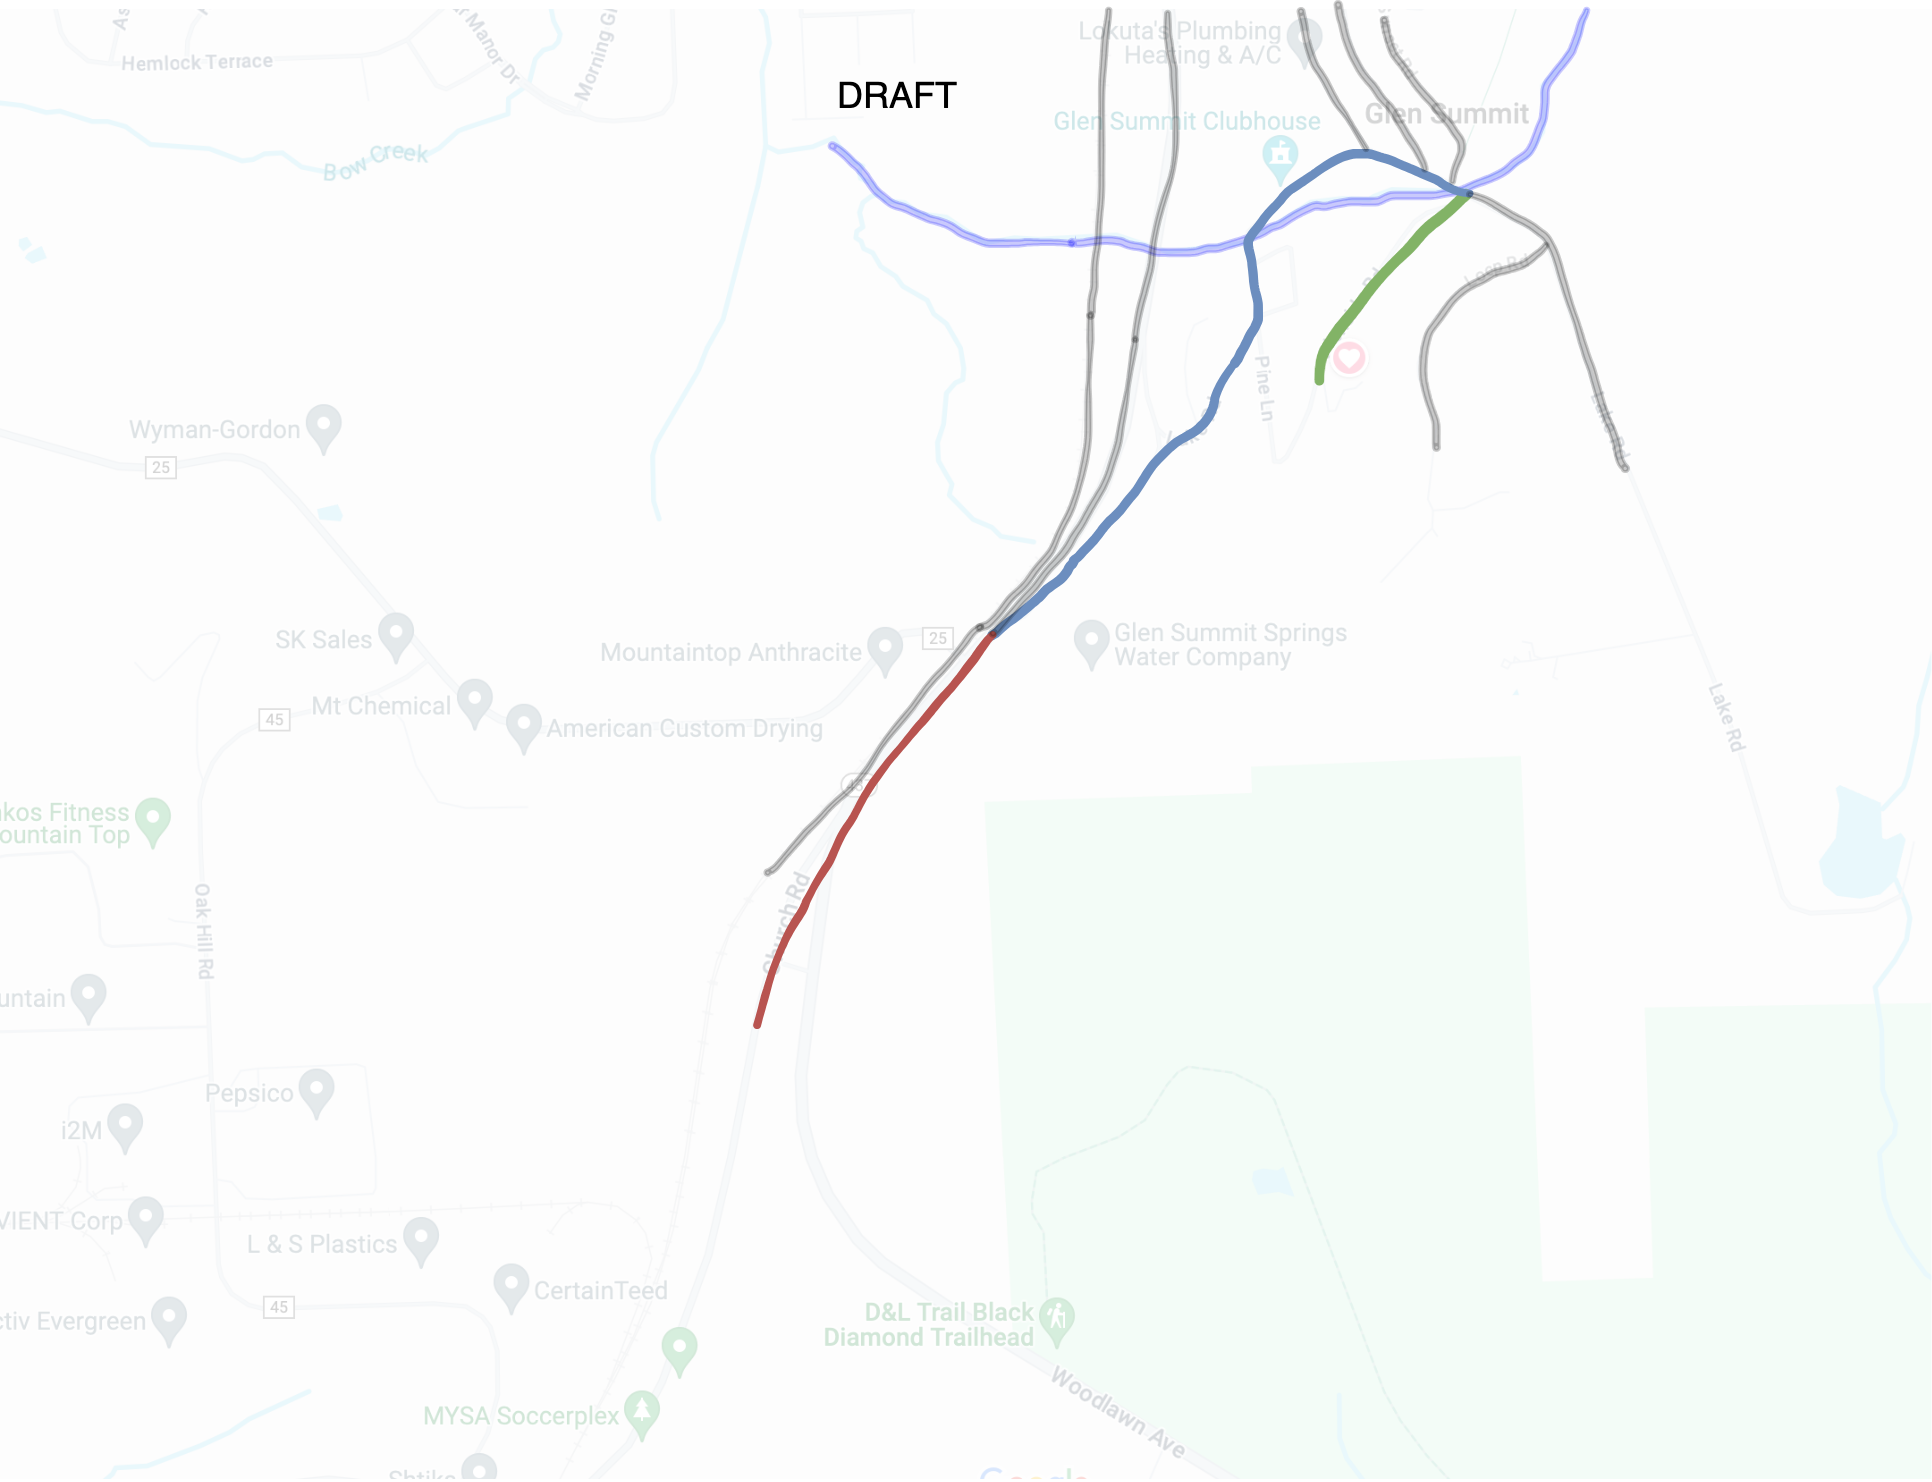
\includegraphics[width=\textwidth]{assets/street-diagram.drawio.png}

\part{Compilation to Machine Learning Accelerators}
\label{part:glenside-and-3la}
  
\chapter{Background and Related Work}
\label{sec:part1-background}

In \cref{part:glenside-and-3la}
  of this dissertation,
  we have described an application
  of our thesis
  to the problem of
  generating compilers
  for deep learning accelerators.
We have described 
  the difficulties in building
  compilers
  for custom accelerators.
First, developing a compiler
  requires much
  developer effort
  and expertise
  (\cref{thesis:devtime}).
Second,
  even once a compiler is built,
  optimizations still often
  get left on the table
  (\cref{thesis:optimizations}).
And lastly,
  the difficulties in
  building compilers
  for accelerators
  often makes the process
  of validation
  of accelerators
  hard if not impossible
  for accelerator designers
  (\cref{thesis:correctness}).
We describe how
  we applied our thesis
  to produce
  \g,
  a domain-specific language
  which can be used to 
  automatically compile
  workloads to accelerators.
We used \g to build
  3LA, a new methodology
  for accelerator design.

We now present background
  and related work
  on the various topics
  involved in
  \cref{part:glenside-and-3la}
  of this dissertation.
We start from the basics, discussing
  existing
  machine learning accelerators
  (\cref{sec:part1:relatedwork:accelerators}),
  whose popularity
  is the core motivation
  behind building 3LA and \g.

\section{Machine Learning Accelerators}
\label{sec:part1:relatedwork:accelerators}

A variety of accelerators~\cite{
    jouppi2017tpu, chen2016eyeriss, moreau2018vta, markidis2018tensorcore, nvdla,
    genc2021gemmini}
  have been developed 
  to provide efficient implementations
  of tensor operators for ML applications.
These devices accelerate tensor operators 
  through hardware parallelism, 
  simultaneously applying related operations
  across many tensors in the accelerator's memory (which are often laid out according to custom rules that facilitate hardware optimization).
  %in the accelerator's memory,
  %often laid out according to custom rules
  %that facilitate hardware optimization.
Tensor program compilers must translate
  expensive application code fragments
  down to accelerator invocations that
  adhere to these layout rules,
  which often involves both
  (a) higher-level transformations like
  tensor reshaping to match accelerator size bounds and
  loop unrolling to expose optimization opportunities, and
  (b) lower-level transformations like
  operator fusion and \tcd{im2col}
  to match accelerator calling conventions and
  even implement different operations
  using the same accelerator,
  e.g., on systolic arrays~\cite{im2col, jia2014semantic}.
  
% Hence, it becomes the task of the compiler 
%   to ensure that data 
%   can be efficiently offloaded 
%   to these accelerators 
%   in the expected format,
%   sometimes requiring higher-level program transformations
%   to avoid redundant transformations.
% \hl{Maybe this isn't the place for im2col?} Additionally, 
%   certain layout transformations 
%   can be used to implement different operations using the same accelerator,
%   as in the above-mentioned \tcd{im2col} example.

\section{Validating Hardware Designs}

\Gls{validation} of hardware designs
  is an incredibly important task---%
  so important, in fact, that it often represents
  a majority of the cost
  for a new hardware design \hl{cite this}.
Validating a hardware design
  is the process of ensuring
  that it behaves as intended.
In the world of hardware design,
  this process is more commonly
  referred to as
  \textit{verification---}%
  however, in this dissertation,
  I prefer to use the definitions
  of \textit{validation} and \textit{verification}
  from the field of Programming Languages,
  in which \textit{validation}
  refers to non-formal-methods-based,
  (usually) non-exhaustive sanity checking,
  while \textit{verification}
  refers to formal, mathematical
  proving of properties (like correctness).
Hardware designers and validation engineers
  perform validation
  at many points in the hardware design process.
For example,
  they might validate that
  their initial prototype of the design,
  written in e.g.~Python or C++,
  behaves identically to their
  initial Verilog implementation
  using a simulator
  such as Verilator~\cite{verilator}.
Later in the design process,
  they might
  formally verify the equivalence
  of their initial Verilog implementation
  against a lower-level,
  backend-specific version of the Verilog
  using an equivalence checker
  like Cadence's Jasper~\cite{jasper},
  or similar tools from Mentor Graphics
  or Synopsys.


Simulation tools can operate
  at different levels of specificity.
Tools like Verilator~\cite{verilator} and Cuttlesim~\cite{pitclaudel2021cuttlesim} enable \textit{cycle-accurate RTL simulation}:
  i.e.~they simulate exactly what the hardware
  is doing
  at each clock cycle.
However,
  cycle-accurate simulation is slow,
  as it requires simulating
  every component within the hardware design.
Often, it is useful to run
  \textit{application-level co-simulation,} 
  in which a high-level software program
  (e.g.~a deep learning model)
  is simulated simultaneously with the hardware.
Co-simulation is integral
  to the 3LA methodology---%
  by running entire applications
  via co-simulation, 3LA helps designers
  find bugs in their hardware designs.
In general, cycle-accurate simulators
  are too slow to run full applications
  in any realistic amount of time,
  making co-simulation infeasible.
In these cases,
  higher-level, non-cycle-accurate simulation
  can enable fast simulation.
SystemC~\cite{SystemC}
  and ILA~\cite{todo},
  are common tools for implementing
  these high-level models.
The 3LA framework relies on ILA, which,
  unlike SystemC,
  provides
  a clear formal verification path to RTL.
  
% Other work has targeted formal verification of code generation for accelerators~\cite{AtlPopl22,ExoPldi22}, but does not have a path to RTL design verification that is possible with ILAs. 
 %and
 %do not support %for %flexible matching and 
 %application-level co-simulation. \sm{Not sure how this fits here.} 
%
  

\section{Hardware--Software Co-Design}

\textit{Hardware--software co-design}
  refers to a loosely grouped
  set of techniques and ideas
  centered around one primary idea:
  rather than the well-defined separation
  between software and hardware design
  which existed in the past,
  hardware and software
  should instead be designed \textit{together.}
That is, to maximize
  the performance of hardware,
  hardware designers should be able to suggest
  changes to the software
  such that it will be more amenable to acceleration;
  similarly,
  software designers should be able to suggest
  hardware changes
  to enable new algorithms.
\g and the 
  \TLA methodology enable
  hardware--software co-design
  through the simple fact that
  they make
  hardware design iterations quicker.
By making it quicker and easier
  to simulate full end-to-end
  applications
  on prototype hardware,
  3LA and \g enable designers
  to see simulation results more quickly
  and adjust both their design
  and the software running on the hardware.

There exists much other work on
  hardware--software codesign
  for deep learning.
Work on accelerator generation and integration~\cite{
    bahr2020creating, truong2020fault}
  has explored adding support in the Halide~\cite{ragan2013halide}
  compiler flow for specialized Coarse-Grained Reconfigurable Array (CGRA) accelerators.
That work composes an
  impressive array of custom tools to
  generate and verify specialized CGRA accelerators
  and also map Halide program fragments
  down to accelerator invocations.
HeteroCL~\cite{lai2019heterocl} also provides
  a similar custom flow.


\section{Tensor IRs and Compilers}

\g, the primary contribution
  of \cref{part:glenside-and-3la}
  of this dissertation,
  is fundamentally an
  intermediate representation (IR)
  for tensor programs.
On top of the \g IR,
  we build the 3LA methodology,
  which includes a compiler
  utilizing \g
  to map deep learning workloads
  to accelerators.
In this section, we describe
  other IRs and compilers
  for tensor programs.

Machine learning workloads
 are generally viewed
 as a sequence of 
 of \textit{tensor kernel} invocations,
 where tensor kernels
 are large operations
 over multidimensional arrays (tensors)
 such as 2D convolution
 or dense matrix multiplication.
Machine learning frameworks
 (such as TensorFlow \cite{tensorflow}
   and PyTorch \cite{pytorch})
 and machine learning compilers
 (such as TVM \cite{chen2018tvm})
 can optimize
 machine learning workloads
 at a number of levels,
 which often result
 in each framework
 having a number of different IRs.
TVM, for example,
 can optimize machine learning workloads
 at a high-level
 using its high-level IR
 Relax~\cite{lai2023relaxcomposableabstractionsendtoend}
 (and its former high-level
   IR Relay \cite{relay}),
 but
 low-level optimizations
 such as loop blocking and reordering
 must be done 
 in its lower-level IRs.

% \hl{not mentioning hand-optimized kernels like CuDNN,
% but maybe that's OK for focus / space}

Tensor compilers for ML and HPC applications strive
  to balance clear, high-level operator semantics
  and support for the low-level optimizations
  necessary to target specialized accelerators.
Halide~\cite{halide}
  achieves this balance by separating
  operator \textit{specifications} (what is computed) from
  \textit{schedules} (how, when, and where
  each output element is generated).
This style of separation has proven
  highly effective across both
  application domains and hardware targets;
  numerous compilers including TVM~\cite{chen2018tvm},
  FireIron~\cite{hagedorn2020fireiron},
  LIFT~\cite{lift}, and Accelerate~\cite{accelerate}
  follow variations of this strategy.
  
The specification/schedule separation approach
  allows the same high-level program (specification)
  to be flexibly optimized for and mapped to
  different hardware targets by applying different schedules.
From this perspective,
  schedules represent different rewriting strategies
  to explore various loop ordering and memory layouts;
  in LIFT and Accelerate these
  take the form of functional combinators
  closely related to \g's approach.
As in classic term rewriting,
  experts must often carefully craft
  schedules for each target to achieve
  the best performance and mitigate
  phase ordering challenges~\cite{phase-ordering},
  though recent projects have produced promising results
  in automatic scheduling~\cite{
    chen2018autotvm, zheng2020ansor, anderson2020learning}.

Other tensor IRs like
  TACO~\cite{taco}, Keops~\cite{keops},
  and COMET~\cite{tian2021highperformance}
  rely on \textit{index notation}\footnote{
    Index notation is closely related to
    ``Einstein notation'', in which reduction
    indices are implicit.}
  to concisely express tensor operators
  and simplify optimization by
  uniformly representing
  per-output-element computations.
These approaches also rely on
  rewriting passes to generate
  kernel implementations specialized to
  tensor sparsity/density,
  operator combinations arising in
  the source application, and
  details of the target hardware.
In Section~\ref{sec:matmul} we discuss
  some of the tradeoffs of these approaches
  with respect to other rewriting strategies.
 
Polyhedral compilers~\cite{polyhedral-survey}
  like Tensor Comprehensions~\cite{vasilache2018tensor}
  and Tiramisu~\cite{tiramisu}
  optimize loop-filled programs
  by modeling loop nests as polyhedra
  and applying geometric transformations.
The polyhedral approach exploits
  regular loop structure,
  but is also restricted
  to geometrically affine transformations.
In contrast, term rewriting is
  neither guided nor restricted by
  geometric constraints, making
  these approaches broadly complementary.


% Accelerators and parallel architectures 
%   present many opportunities 
%   for tuning and improving tensor operator implementations for the best performance.
% Many systems, 
%   including deep learning frameworks like PyTorch~\cite{pytorch},
%   make extensive use of hand-optimized tensor operator implementations
%   (such as those in the CuDNN library~\cite{chetlur2014cudnn}).
% While these hand-optimized implementations
%   achieve strong performance,
%   various systems, including \g,
%   have been proposed to automatically
%   generate optimized tensor operators
%   to reduce development time,
%   support varied hardware platforms,
%   and avoid reliance on a small number of experts.
% These tensor compilers 
%   rely on specifying tensor computations 
%   in a form that allows for
%   conveniently exploring options for optimizations, 
%   such as by changing loop orderings
%   to best utilize caches.

% \hl{Surely there's a better summary/gloss here.}
% Many tensor operator compilers 
%   use index notation
%   to specify tensor operators
%   (defining how each element of the output
%   is to be computed
%   based on corresponding elements 
%   of the input).
% TACO~\cite{taco} uses index notation 
%   for automatically generating and optimzing both sparse and dense tensor computations,
%   permitting particular dimensions 
%   to be specified as dense or sparse,
%   introducing various structures for reasoning about how 
%   to iterate over sparse dimensions.
% %Tensor operators in TACO
%   %are described using index notation, 
%   %with particular tensor dimensions 
%   %being either dense or sparse.
% %\cite{taco} initially 
%   %focused on compiling for CPU, 
%   %while subsequent work~\cite{senanayake2020}
%   %has extended TACO to target
%   %GPUs and vector units.
% %  is a compiler notable for its handling
% %  of computations over sparse tensors.
% %\hl{unsure how to draw any connection here, but i feel like i need to at least mention taco}
% Keops~\cite{keops} also uses
%   index notation to describe tensor operations
%   for both dense and spare matrices,
%   but introduces another matrix representation
%   called symbolic matrices, 
%   in which each element of the symbolic matrix
%   is computed from two smaller data matrices.
% Computations on symbolic matrices 
%   can more easily be deployed to GPUs and other accelerators 
%   than sparse computations
%   but require less data movement than dense computations.
% %% I think MLIR isn't relevant in this discussion: IRs built _in_ MLIR might be
% %MLIR~\cite{mlir} is a general-purpose compiler framework intended to facilitate the development of IRs.
% %While MLIR itself does not have a built-in notion of tensorization, it has been used to implement polyhedral IRs and other tensor operator representations.
% COMET~\cite{tian2021highperformance} is another
%   CPU-focused sparse tensor algebra IR,
%   implemented using MLIR~\cite{mlir},
%   that additionally uses information about sparse storage formats 
%   in its representation 
%   to increase temporal and spatial locality.

% Halide~\cite{ragan2013halide}
%   %while not a machine learning compiler
%   has been influential
%   in using a representation
%   that separates
%   an tensor operator's specification (what it computes)
%   from its schedule (what order elements are computed),
%   allowing many optimizations
%   to be described as different schedules
%   for the same specification
%   and facilitating operator fusion.
% As discussed in~\cite{newcomb2020halide-rewrite},
%   Halide applies a term rewriting system
%   for producing optimized code.
%   \hl{Any insight for why Halide is amenable to a rewrite system?}
% TVM~\cite{chen2018tvm}
%   uses a similar specification-schedule split
%   for describing its tensor operators.
% FireIron~\cite{hagedorn2020fireiron} is another system
%   using a split between a computation specification 
%   and its realization
%   (using a decompositions, rather than Halide-style schedules,
%   for scheduling parts in a top-down style).
% \g can be understood
%   as a further refinement
%   on an algorithm's specification,
%   disambiguating
%   how data is accessed
%   from the computation being performed
%   over the data,
%   enabling transformations
%   like mapping to hardware
%   before the program is scheduled.
%   \hl{What does it mean
%   that mapping to hardware
%   is done before the program is scheduled?}

% Like \g, several other systems 
%   use functional representations
%   of tensor operators.
% LIFT~\cite{lift}
%   separates specifications from schedules
%   using combinators like maps and reductions to specify schedules,
%   an idea further explored in~\cite{hagedorn2020func-high-perf}.
% \hl{anything else to say about LIFT? Contrast with Halide/TVM's scheduling languages?}
% Accelerate~\cite{accelerate} 
%   uses functional combinators 
%   to map Haskell code 
%   to GPU programming primitives.
% \hl{Discussion comparing these to \g?}

% The polyhedral representation~\cite{polyhedral-survey} 
%   has also proven useful
%   for expressing tensor operators.
% %Polyhedral compilation~\cite{polyhedral-survey}
%   %is a powerful alternative
%   %to term rewriting-based compilers.
% Polyhedral compilers optimize
%   loop-filled programs
%   by modeling loop nests
%   as polyhedra
%   and transforming them geometrically.
% Tensor Comprehensions~\cite{vasilache2018tensor}
%   and Tiramisu~\cite{tiramisu}
%   are examples of machine learning compilers
%   powered by the polyhedral framework.
% \hl{Need note about deploying to accelerators?}
% \hl{Implications for term rewriting?}
% Multidimensional homomorphisms~\cite{multidimensional-homomorphism} 
%   are another mathematical representation 
%   of tensor operations
%   that has been amenable to automatic parallelization 
%   and allows for hierarchical composition.
%   \hl{any comment in relation to \g?}

%There are at least as many
  %tensor IRs
  %as there are
  %deep learning frameworks,
  %and many frameworks
  %use more than one.
%TVM \cite{chen2018tvm},
  %for example,
  %uses the high-level
  %Relay IR~\cite{relay}
  %for optimizations
  %in the sequencing of tensor kernels,
  %while it uses low-level TIR
  %to optimize kernels themselves.
%\hl{If you're going to complain about TIR not being pure, you need to establish that purity is a requirement before this. Maybe discuss this later}
%Relay and TIR
  %are a perfect example
  %of our impedance mismatch problem:
  %Relay is pure but too high-level,
  %while
  %TIR is low-level but impure.


% Should we talk about BYOC here?
%Recently,
%  the Bring Your Own Codegen
%  (BYOC)
%  framework
%  was merged into TVM \cite{byoc}.
%BYOC
%  is novel,
%  as it allows for the 
%  fast implementation
%  of a full compiler
%  for deep learning models
%  down to custom hardware backends
%  with fairly little additional code,
%  assuming the users
%  have written a codegen
%  for their hardware
%  already.
%BYOC includes
%  a matching framework,
%  for matching
%  user-specified
%  patterns
%  of Relay code.
%As we will see
%  in Section \ref{sec:case-study-tensorization},
%  one of our primary case studies
%  of \g{}
%  is as a pattern matcher
%  for matching such computational patterns---%
%  in fact,
%  it was the original
%  intended use case
%  of \g{}!
%In some sense,
%  the two pattern matchers
%  are incomparable,
%  because,
%  as we've described above,
%  \g{}
%  and Relay
%  operate at different levels
%  of abstraction.
%Yet if we ignore the differences
%  in the levels of abstraction,
%  we can compare
%  the matchers
%  in how they operate.
%In this comparison,
%  \g{} shines through
%  with the help of
%  the \egr{}.
%Because rewrites
%  are so cheap and easy
%  within the \egr{},
%  we can run a huge number
%  of exploratory rewrites,
%  potentially finding places
%  to map in user-defined
%  patterns.
%BYOC,
%  on the other hand,
%  expects the user to provide
%  multiple equivalent patterns
%  to cover the numerous ways
%  their pattern might appear 
%  in the program
%  \hl{(verify this)}.

%Named tensors \cite{chiang2021named}
%  are a primary inspiration
%  for the access pattern data structure
%  at the core of \g.
%%Tensors have a specific layout
%%  in memory,
%%  a hardware detail
%%  that often bubbles up
%%  even to the highest levels
%%  of tensor abstractions.
%%For example,
%%  in both TVM and TensorFlow,
%%  the \tcd{conv2d} operator
%%  requires the user to specify
%%  the layout of the activation tensor---%
%%  \tcd{NCHW} or \tcd{NHWC},
%%  where \tcd{N} is the batch dimension,
%%  \tcd{C} is the channels dimension,
%%  and \tcd{H} and \tcd{W} are the spatial
%%  (height and width)
%%  dimensions.
%%Rather than pass layout information
%%  externally,
%%  named tensors
%%  incorporate dimension names
%%  directly into the tensor abstraction.
%%Named tensors
%%  acknowledge the fact
%%  that
%%  not all dimensions
%%  are made the same,
%%  and that different dimensions
%%  have different functions.
%Named tensors
%  assign names
%  to the dimensions of a tensor,
%  increasing code readability
%  and acknowledging that different dimensions
%  have different functions.
%Though
%  we do not actually adopt
%  this notation
%  in \g{}---%
%  the dimensions of tensors
%  are still just indexed
%  with integers---%
%  this core idea
%  is reflected
%  in the design
%  of access patterns,
%  which encode the fact that
%  some dimensions are
%  for
%  \textit{iterating over,}
%  while others are meant to be 
%  \textit{computed upon.}

%Many machine learning frameworks
  %have an optimization step
  %in which they match program patterns
  %to efficient low-level implementations,
  %whether that be offloading to hardware
  %or calling into a tuned library.
%TVM \cite{chen2018tvm}, 
%% Steve: I would say Latte is not very relevant here
%% It provides AD, but it requires the user to manually implement just about everything else
  %Latte \cite{latte},


%% Steven: Not clear it's relevant to this context
%Norman Ramsey instruction selection~\cite{dias2010instruction-selection}

%\hl{even further back:} apl?~\cite{apl-survey} % probably no


Another key piece of background to note
  when it comes to deep learning compiler frameworks
  is interoperability of frontends.
Machine learning models can be expressed
  in many frontend languages,
  including MxNet~\cite{chen2015mxnet},
  PyTorch~\cite{paszke2019pytorch},
  TensorFlow~\cite{abadi2016tensorflow},
  ONNX~\cite{linux2019onnx},
  and CoreML~\cite{apple2022coreml},
  and generally,
  compilers should strive to support
  models expressed in all of these frontends.
As it is built on top of TVM,
  which supports importing from many
  frontend languages,
  our \TLA prototype
  supports all of these frontend languages.
  
% \TLA is capable of supporting any accelerator back-end provided that it be represented in terms of ILA instructions. BYOC, MLIR, and Exo are similarly capable of supporting arbitrary back-ends, so long as users implement custom code generators. Several Halide extensions have implemented support for some accelerators, like stencils or systolic arrays, but these have required modifications to Halide's core (see Table~\ref{figure.methodology}).
% %and are not extensible with respect to new back-ends. 
% While Glenside can represent arbitrary accelerator operations as opaque predicates, no further code generation is implemented (hence, \TLA is its first use in code generation).

% Formally verified compilers such as  
%   CompCert~\cite{leroy2006formal} and CakeML~\cite{kumar2014cakeml}
%   can rigorously establish end-to-end equivalence
%   from high-level source code down to assembly for
%   various CPU back-ends via machine-checkable proofs,
%   but currently do not provide a general approach
%   for integrating new accelerator support and
%   provide no support for custom numerics.
% In contrast, \TLA enables validating
%   accelerator mappings via
%   end-to-end simulation handling custom numerics. 
  %and formally verifying individual rewrite rules from compiler IR patterns to accelerator invocations.
% \TLA provides an approach
%   to extend existing compilers
%   with mappings from DSLs workloads
%   to custom accelerator back-ends and
%   enables validating these mappings
%   via end-to-end simulation.
% Thus, \TLA complements
%   existing compiler verification efforts, and
%   may provide guidance for future work on formally
%   verifying ``accelerator-extensible'' compilers.


  
%   \hl{Need to make sure that we distinguish \TLA's validation of the compilation results from the CompCert style verifying the compiler itself.}



%\subsection{Term Rewriting, Equality Graphs, and Equality Saturation}
\subsection{Term Rewriting and Equality Saturation}

Term rewriting is a classic
  program optimization technique~\cite{baader1998term}
  that relies on iteratively applying
  rewrite rules of the form $\ell \xrightarrow{} r$:
  when part of a program
  matches the pattern $\ell$
  under substitution $\sigma$,
  it is rewritten into $\sigma(r)$.
This approach is ubiquitous,
  frequently used in both mainstream and DSL compilers
  to implement features including preprocessing,
  strength reductions, and
  peephole optimizations~\cite{garavel2018rewrite-context}.
  
Classic term rewriting systems where
  rewrites are applied destructively suffer
  phase ordering problems~\cite{phase-ordering}:
  the order in which rewrites are applied can
  enhance or severely diminish performance.
Recent work has shown how program synthesis
  can help address this challenge in
  peephole optimizers like Halide's
  scalar expression rewriter~\cite{
    newcomb2020halide-rewrite}.
  
Advances in alternate rewriting techniques
  like equality saturation~\cite{tate2009equality}
  also mitigate phase ordering by exploiting
  the e-graph data structure from SMT solvers
  to repeatedly apply all rewrites simultaneously,
  thus obviating rule ordering considerations.
In particular,
  the \tcd{egg} library~\cite{willsey2021egg}
  has been used to develop new synthesis and
  optimization tools across diverse domains~\cite{
    herbie, szalinski, wang2020spores},
  including DSP compiler vectorization~\cite{
    vanhattum2021vectorization} and
  tensor computation graphs~\cite{yang2021equality}.

\g provides the first tensor IR
  amenable to equality saturation by
  introducing access patterns to
  provide pure, higher order tensor
  kernel combinators that support
  rank-polymorphism without the need
  for binding structures like
  anonymous functions or index notation.

% {\color{red} \noindent\rule{8.5cm}{10pt}}

% \g utilizes
%   the power of equality saturation
%   in
%   low-level tensor program
%   transformation---%
%   namely, mapping programs
%   to custom hardware.
  
% Term rewriting
%   is a classic technique
%   in program optimization
%   in which rewrite rules of the form
%   $\ell \xrightarrow{} r$
%   are applied over a program.
% When an expression in the program
%   matches
%   the pattern $\ell$,
%   it is rewritten
%   into the pattern $r$.
% In classic term rewriting systems,
%   the ordering
%   in which rewrites are applied
%   can affect whether optimizations
%   are found,
%   as some rewrites
%   may reverse or muddle
%   the effects
%   of other rewrites.
% Equality saturation
%   is a technique
%   developed to sidestep
%   this 
%   phase ordering problem.
% The technique
%   has recently re-emerged
%   with the development
%   of the \tcd{egg} library
%   \cite{willsey2021egg},
%   and with the successful application
%   of equality saturation
%   to floating point optimization \cite{herbie}
%   and CAD program simplification \cite{szalinski},
%   among other varied fields.

% %A primary feature
% %  of equality saturation
% %  is its ability to
% %  efficiently store
% %  all previously discovered
% %  versions 
% %  of the program
% %  being transformed.
% %The data structure which enables this
% %  is the
% %  \textit{equality graph}
% %  (\egr),
% %  which resembles
% %  a standard program graph (\hl{not sure on words to use here?}),
% %  except
% %  each node in the program
% %  is replaced with a \textit{set} of nodes,
% %  called an \textit{equivalence class}
% %  or \textit{eclass.}
% %All nodes within an eclass
% %  are equivalent, and thus 
% %  can be substituted for one another
% %  to produce an equivalent program.
% %This property is only possible
% %  when the language used
% %  within the \egr
% %  is pure,
% %  which thus becomes a requirement
% %  for any language
% %  we'd like to transform
% %  with equality saturation.
  
% Diospyros \cite{vanhattum2021vectorization}
%   is a vectorizing compiler
%   for DSPs
%   which uses equality saturation
%   to match program fragments
%   to hardware primitives.
% Diospyros
%   starts from scalar programs
%   and, via symbolic evaluation
%   and equality saturation,
%   lifts them to vectorized
%   expressions,
%   while \g starts
%   from a higher level of abstraction
%   and searches downwards.
  
% SPORES \cite{wang2020spores}
%   and Tensat \cite{yang2021equality}
%   utilize equality saturation
%   to optimize
%   linear algebra expressions
%   and tensor computation graphs,
%   respectively.
% While both
%   show the potential
%   of equality saturation
%   for tensor program transformation,
%   both of their IRs
%   are too high-level
%   for the task of mapping to hardware.

% TODO mention somewhere in here that lambdas (which a lot of langs will use) are a problem for first-order rewrite systems

\subsection{Pattern Matching Accelerator Calls}

The most closely related work to flexible matching is from 
   TVM BYOC~\cite{chen2021byoc}, which only provides exact syntactic matching as discussed in \S\ref{sec.background}.
Past work has also explored rewrite-based techniques for
  automatically inferring instruction selection passes
  between ISAs~\cite{
    ramsey2011resourceable,
    dias2010automatically}
  and in the context of superoptimization~\cite{
    bonsal-so,
    bonsal-so-translate}.
Rewriting in \TLA instead operates on a high-level IR
  to expose opportunities to invoke code generators,
  rather than performing low-level code generation directly.
Equality saturation has been
  used in the context of
  ML and DSP compilers for
  optimization~\cite{
    yang2021equality,
    alexa-dsp-eqsat,
    caviar-cc22}.
There has also been significant work on
  ML and HPC compiler frameworks with
  varying degrees of support for
  targeting custom accelerators~\cite{
    ragan2013halide,
    AtlPopl22,
    chen2018tvm,
    moreau2019hardware,
    lattner2021mlir}.
To the best of our knowledge,
  none of these frameworks provides support for
  testing prototype accelerators
  designs end-to-end on
  unmodified source applications.
  


% In principle, many DSLs allow for supporting custom accelerators via bespoke translations from DSL operators to specific accelerator APIs,
% e.g., as in the original TVM~\cite{chen2018tvm} support for VTA~\cite{moreau2019hardware}.
% %
% TVM's BYOC~\cite{chen2021byoc} interface
% % provides a more convenient mechanism for
% eases incorporating custom accelerators
% %, especially for coarser-grained operations,
% by performing syntactic pattern matching to offload computations via user-provided code generators.
% % By building on TVM,
% %   BYOC inherits support for multiple frontends
% %   and additionally provides extensible pattern matching to facilitate
% %   adding new rules for mapping DSL fragments to new accelerators.
% %\hl{merge next two sentences?}
% However, BYOC leaves
%   all matters of code generation, e.g., MMIO invocations,
%   to the user,
%   while \TLA provides
%   more structure to code generation
%   via the ILA.
% %Furthermore, unlike \TLA, BYOC does not directly support custom
% % code generation for fine-grained MMIO invocations.
% In particular, 
%   the ILA provides useful simulation capabilities.
% %   that can be of practical use during compiler development, 
% %   whereas any comparable faculties (such as TVM's built-in VTA functional simulator) 
% %   would otherwise have to be separately developed and deployed.
% Additionally, BYOC's pattern matching
% %, while incorporating some dataflow analysis beyond exact matching,
% cannot search the space of programs equivalent to the input,
% limiting the number of potential accelerator invocations %it can find
% compared to flexible matching in our \TLA prototype.

% The MLIR framework~\cite{lattner2021mlir} provides a rich metalanguage and numerous tools for
%   developing, optimizing, and translating between custom compiler IRs,
%   but does not inherently provide direct support for
%   \TLA's features.
%   %--- MLIR serves more as a rich metalanguage
%   %in which users can develop custom IRs,
%   %potentially reusing tools and definitions.
%   %ideally reusing tools and definitions from related IRs also
%   %expressed in MLIR.
% It would be possible to realize the \TLA methodology
%   within an MLIR-based ecosystem; 
%   we implemented our DL-focused prototype using TVM %and BYOC
%   since it allowed leveraging 
%   % us to leverage 
%   more DL infrastructure.
%   %in the case of our DL-focused prototype, 
%   %we found it more convenient to use TVM and BYOC 
%   %we believe that our current approach using BYOC required less effort and derived more benefit
%   %from existing infrastructure. 
%   %\hl{Not sure what is the point being made in the later part of this sentence. --It is supposed to explain why we chose to implement our prototype via TVM rather than MLIR. Can rephrase to clarify}

% However, these instruction selection techniques
%   are complementary to \TLA's approach
%   and potentially can be used in the \TLA methodology
%   for generating instructions for fine-grained accelerators like VTA.
%\hl{maybe add sentence distinguishing from flex matching, and then cut what is now the last sentence of this para?}
%   and how equality saturation can be applied
%   to automatically discover accelerator opportunities~\cite{willsey2021egg}. \hl{Should the cite at the end be Glenside? Not sure what in the egg paper it is referring to.}
%These techniques provide an ideal complement to
%  \TLA's pattern-matching approach and could be
%  incorporated into the \TLA methodology in future work.
%   for generating instructions for fine-grained accelerators like VTA.


% \subsubsection{The Costs and Benefits of Abstraction in 3LA}
% %
% In order to provide modularity, extensiblity, and verification,
%   the 3LA methodology relies on ILA-based abstractions of both
%   compiler IR intrinsics and accelerator operations.
% Our earlier case studies (Section~\ref{sec.eval}) demonstrate
%   the numerous benefits such abstractions can provide,
%   but the approach is not a panacea.
% In particular, strictly respecting abstraction boundaries in 3LA
%   complicates adding support for lower-level optimizations like
%   operator fusion that require fine-grained knowledge of operator internals.
% %  operator fusion that requires first ``inlining'' low-level
%   %operator implementations to expose optimization opportunities.
% This added complexity does not impact coarse-grained accelerators
%   like FlexASR, but further work may be required to achieve
%   optimal performance for finer-grained accelerators.
%   %that rely
%   %on operator fusion.







  
  
  
  
  
  



% ---------- CASES ----------

% \section{Related Work} \label{sec.related}

% The 3LA methodology uses the ILA as a uniform interface
%   connecting DSLs to custom accelerators by
%   incorporating an extensible pattern matcher to verifiably
%   map application fragments to accelerator invocations.
% As such, 3LA is closely related to both
%   various mainstream systems and
%   past work on
%   software/hardware co-design,
%   extensible compiler frameworks, and
%   compiler verification.

% \subsection{Relation to Current Approaches}
% %
% Table~\ref{tab.comparison} provides
%   a high-level comparison of 3LA to
%   a selection of related methodologies, tools, and frameworks.
% Because 3LA spans several layers of the system stack,
%   these contrasting points are not all of the same sort;
%   we discuss the nuances of such ``cross-category''
%   feature comparisons below.

% \mysubsub{Representative Approaches and Key Features.}
% %
% Calling back to Section~\ref{subsec.challenges},
%   we consider how each related approach supports
%   formal software/hardware interfaces (Formal SW/HW),
%   verification (Verif),
%   end-to-end workflows (E2E),
%   multiple backends (Multi-Back),
%   multiple frontends (Multi-Front),
%   extensible pattern matching (PatMatch), and
%   compiler optimizations (Opts).
% Across these dimensions, we compare
%   traditional, manual approaches to customization (Ad Hoc),
%   the TPU support provided in the
%     TensorFlow~\cite{abadi2016tensorflow} (TPU: TF) and
%     PyTorch~\cite{paszke2019pytorch} (TPU: PT) frameworks,
%   the BYOC interface~\cite{chen2020byoc}, and
%   the MLIR framework for developing compiler IRs~\cite{lattner2021mlir}.


% \input{tab_comparison.tex}


% \mysubsub{Comparing Approaches.}
% %
% Table~\ref{tab.comparison} highlights two
%   of 3LA's key benefits relative to  existing approaches:
%   providing a formal software/hardware interface and
%   built-in verification support via ILAng~\cite{huang2019ilang}.
% Traditional, ad hoc approaches and implementations providing
%   custom accelerator support for a particular DSL
%   (TPU: TF, TPU: PT) can map from high-level DSLs all the way
%   to MMIO-invoked custom accelerators,
%   but generally are too specialized to provide easy extensibility.
% However, such focused specialization also facilitates
%   good support for compiler optimizations, both
%   at higher levels (HL, e.g., common subexpression elimination) and
%   at lower levels (LL, e.g., operator fusion).

% By building on the TVM framework,
%   BYOC inherits support for multiple backends and frontends and
%   additionally provides extensible pattern matching to facilitate
%   adding new rules for mapping DSL fragments to new accelerators.
% However, BYOC leaves
%   all matters of code generation, e.g., MMIO invocations,
%   to the user,
%   while 3LA provides
%   more structure to code generation
%   via the ILA.
% %However, unlike 3LA, BYOC does not directly support custom
% %  code generation for fine-grained MMIO invocations.

% The MLIR framework provides numerous tools for
%   developing, optimizing, and translating between custom compiler IRs,
%   but does not inherently provide direct support for any of
%   the features 3LA targets --- similarly to BYOC, MLIR serves more as a rich metalanguage
%   in which users can develop custom IRs,
%   potentially reusing tools and definitions.
%   %ideally reusing tools and definitions from related IRs also
%   %expressed in MLIR.
% It would likely also be possible to realize the 3LA methodology
%   within an MLIR-based ecosystem; in the case of our DL-focused
%   prototype, we believe that our current approach using BYOC required less effort and derived more benefit
%   from existing infrastructure.
 
% \mysubsub{The Costs and Benefits of Abstraction in 3LA}
% %
% In order to provide modularity, extensiblity, and verification,
%   the 3LA methodology relies on ILA-based abstractions of both
%   compiler IR intrinsics and accelerator operations.
% Our earlier case studies (Section~\ref{sec.eval}) demonstrate
%   the numerous benefits such abstractions can provide,
%   but the approach is not a panacea.
% In particular, strictly respecting abstraction boundaries in 3LA
%   complicates adding support for lower-level optimizations like
%   operator fusion that require fine-grained knowledge of operator internals.
% %  operator fusion that requires first ``inlining'' low-level
%   %operator implementations to expose optimization opportunities.
% This added complexity does not impact coarse-grained accelerators
%   like FlexASR, but further work may be required to achieve
%   optimal performance for finer-grained accelerators.
%   %that rely
%   %on operator fusion.

% \subsection{Broader Related Work}

% % 3LA additionally relates to broader research efforts
% %   across the system stack.
% % Below we briefly highlight some of
% %   the most closely related past work.

% \mysubsub{Software/Hardware (SW/HW) Co-Design.}
% %
% Recent work on accelerator generation and integration~\cite{
%     bahr2020creating, fault-truong-cav2020}
%   has also explored adding support in the Halide~\cite{ragankelley2013halide}
%   compiler flow for specialized Coarse-Grained Reconfigurable Array (CGRA) accelerators.
% In that approach, the authors compose an
%   impressive array of custom tools to
%   generate and verify specialized CGRA accelerators
%   and also map Halide program fragments
%   down to accelerator invocations.
% HeteroCL~\cite{lai2019heterocl} also provides
%   a similar custom flow.
% %designed around the details of the HeteroCL compiler flow.
% In contrast, the 3LA methodology is design to support
%   fast and flexible SW/HW co-design by mitigating impedance mismatches
%   between the granularity of \textit{independently developed}
%   DSLs and \textit{near-arbitrary} accelerators;
%   because of the flexibility of the ILA,
%   the 3LA methodology is applicable to a
%   broad class of compilers and accelerators,
%   rather than being focused on a single compiler flow
%   or class of accelerators.

% % As such, 3LA complements the above past work in
% %   HW/SW co-design and could be combined with
% %   those approaches to further ease the
% %   development, integration, and verification
% %   of specialized accelerators supporting high-value applications.

% \mysubsub{DSL Design, Extensible Compiler Frameworks, and Compiler Verification}
% %
% Numerous DSLs
%   to facilitate programming productivity
%   in high-value applications have recently become popular, e.g.,
%   TVM~\cite{chen2018tvm},
%   Halide~\cite{ragankelley2013halide}, and
%   TACO~\cite{taco}.
% The 3LA methodology complements all these efforts;
%   3LA is designed to ease adding accelerator support for
%   compilers in this class of high-performance DSLs
%   by providing a uniform interface that can be reused
%   across DSLs and compilers and additionally
%   introduce support for verifying compiler-to-accelerator
%   mappings via ILAng tooling~\cite{huang2019ilang}.

% Past work has also explored rewrite-based techniques for
%   automatically inferring instruction selection passes
%   between ISAs~\cite{dias-isel-popl10}
%   and how equality saturation can be applied
%   to automatically discover accelerator opportunities~\cite{willsey2021egg}.
% These techniques provide an ideal complement to
%   3LA's pattern-matching approach and could be
%   incorporated into the 3LA methodology in future work.

% Formally verified compilers like
%   CompCert~\cite{compcert} and CakeML~\cite{cakeml}
%   can rigorously establish end-to-end equivalence
%   from high-level source down to assembly for
%   various CPU back-ends via machine-checkable proofs,
%   but currently do not provide a general approach
%   for integrating new accelerator support.
% 3LA provides exactly such an approach
%   for extending existing compilers
%   with verifiable mappings from program fragments
%   to accelerator back-ends, and thus also complements
%   the state-of-the-art in formal compiler verification.


% % listing what different approaches provide.
% % Verification, pattern matching, co-design, numerics support, and 
% % integration with broader workflow.

% % Compare with Cosy (Lisa) and Target (nML), manual dev, BYOC, and 
% % MLIR~\cite{lattner2021mlir}.

% % Table~\ref{tab.comparison} listing what different approaches provide.
% % Verification, pattern matching, co-design, numerics support, and 
% % integration with broader workflow.


\chapter{Introduction and Motivation}
\label{sec:part1-motivation}

% Top-level points: 
% We need something like the 3LA methodology;
% 3LA methodology needs flexible matching.


% WE NEED SOMETHING LIKE 3LA METHODOLOGY
% Points:
%% Hardware acceleration is important.
%% Accelerators are nothing without testing/without compilers? which one?
%% Need a methodology for building compilers.

%% Hardware acceleration is important.

Hardware acceleration has powered significant advances
  in subfields like artificial intelligence, image processing, and graph analysis~\cite{han2016eie,chen2016eyeriss,reagen2016minerva,zhang2016cambricon,hameed2010understanding,ham2016graphicionado,jouppi2017tpu, krizhevsky2012conv, reuther2019survey}.
This trend has highlighted the need
  for flexible accelerator support
  in domain-specific compilers like
  Halide~\cite{halide},
  TVM~\cite{chen2018tvm},
  TensorFlow/MLIR~\cite{tensorflow, mlir}, and
  PyTorch~\cite{pytorch}.

Despite our increasing dependence
  on accelerators,
  building compilers
  for custom accelerators
  remains a daunting task.
Paralleling the thesis of this dissertation,
  we will describe the challenges
  of building compilers
  along three axes:
  \cref{thesis:devtime},
  \cref{thesis:optimizations},
  and \cref{thesis:correctness}.
  

\paragraph{
\cref{thesis:devtime}.
}
Current frameworks for compiler generation
  generally require significant compilers expertise,
  and the sheer amount of effort
  required to build a compiler from the ground up
  generally limits bespoke compiler construction
  to teams
  at large companies,
  e.g. the TensorFlow 
  stack~\cite{abadi2016tensorflow}
  for Google's 
  TPU~\cite{jouppi2017tpu,jouppi2020tpu}.
Though projects
  such as 
  MLIR~\cite{mlir,
  lattner2021mlir,
  eldridge2021mlir}
  and
  Exo~\cite{ExoPldi22}
  have begun to prescribe
  a general framework
  for structuring a compiler,
  these tools are built for
  domain experts,
  and require significant time investment
  \hl{vague}.
There is a need for
  automated techniques
  for compiler generation,
  to lower the barrier
  and allow non-experts to generate
  functioning compilers.
An example of such a technique
  is the deep learning compiler
  TVM's~\cite{chen2018tvm}
  Bring Your Own Codegen (BYOC)
  framework~\cite{chen2021byoc}.
\hl{tease at how BYOC will fail? or handle in optimizations?}
Though, 
  as we will show later,
  while BYOC makes it easy for
  users to add basic support
  for accelerators,
  we will see 
  that its ability to 
  match workloads to accelerators
  is lacking.

\paragraph{
\cref{thesis:optimizations}.
}
Even once a compiler is constructed,
  they still have the tendency
  to leave optimizations on the table---%
  especially user-facing compiler construction frameworks.
\hl{As a consequence, optimizations can be left on the table.
Note that simply mapping to accelerators
  is considered an optimization,
  but e.g.~mappings can be missed.}
Even once a compiler
  is constructed
  for a piece of custom hardware,
  it can still leave optimizations
  on the table.
Getting a compiler to realize
  that a certain operator
  can be run on an accelerator,
  for example,
  may require syntactic changes
  to the input program,
  especially when using
  a matcher like
  BYOC.

And the difficulties
  in building a quality compiler
  often lead hardware designers to forego the process
  entirely, which can
  hinder or entirely prevent
  the validation and testing
  of custom hardware,
  leading to expensive bugs
  (\cref{thesis:correctness}).
\cref{thesis:correctness}
Core to developing
  accelerators
  quickly and correctly
  is the process of \textit{hardware validation.}
\hl{glossary terms: validation, testing, verification}
\textit{Validation}
  of hardware---%
  the process of testing
  whether the hardware behaves
  how the designer intended---%
  is important.
An immense amount of effort
  and money
  is currently put
  into hardware validation and testing.
\hl{how much is spent on hw validation compared to sw}  
Despite the growing dependence
  on accelerators,
  testing custom hardware is still largely
  a manual, ad hoc, and difficult process.
A primary challenge in 
  accelerator development
  is validating designs
  on real applications.
This validation
  is critical,
  as some accelerator bugs 
  arise
  only during validation
  of full applications.
For example,
  a deep learning
  accelerator may use
  a custom numeric format
  tuned to be storage-efficient,
  while still providing enough
  precision
  to support effective inference.
Testing the numeric format
  on a single layer
  of the deep learning model
  may produce results
  well within the designer's
  error bounds.
However, if the designer
  neglects to test
  \textit{all}
  layers of the model,
  they may fail to discover that,
  even though individual layers
  behave well,
  the error may accumulate
  across layers
  to an unfeasible degree~\cite{zorn2021rounding}.
Early end-to-end application level validation is thus essential
  for avoiding expensive and complex late stage hardware design changes.
\hl{merge or delete below}
In general,
  thorough validation
  is inaccessible
  to the common designer.
The most intensive validation
  is done in industry,
  where companies can hire full-time
  engineers
  to do validation
  on designs.
\hl{reference fig} \cref{fig:3la-pie}

\begin{figure}
\centering
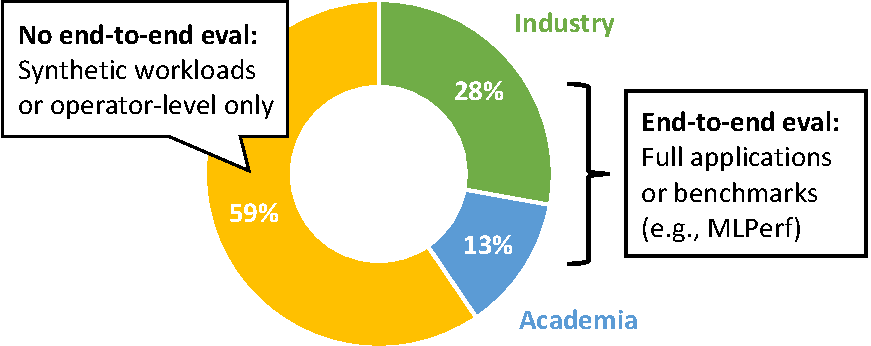
\includegraphics[width=.6\textwidth]{assets/3la-pie.pdf}
\caption{
\hl{this figure is taken from ...cite 3LA...update caption}
\textbf{Gap in end-to-end evaluation of accelerators for neural network applications:} 
Survey of papers from ISCA, MICRO, VLSI, and ISSCC in 2021 and ICCAD, DAC in 2020.
Our survey of $79$ papers  that introduced new DL accelerator designs/methodologies, comparing how the accelerators were evaluated. Only 41\% of the works reported end-to-end evaluation on non-synthetic applications, of which 68\% (28\% of the total) were from industrial teams.
}
\label{fig:3la-pie}
\end{figure}


  
When validation \textit{is} done
  outside of industry,
  it is often not done end-to-end.
Not only is it important
  to test \textit{components}
  of a hardware design;
  it is also important
  to test full applications end-to-end.
Hardware specialization and customization often
  requires changing memory hierarchies,
  data representations~\cite{chan2014itrs,fang2019understanding,lai2021programming}.
Issues arising from these complex
  microarchitectural changes
  may not manifest
  at the component level---%
  for example, a reduced-bitwidth
  ALU
  may still produce accurate results,
  but overall \textit{application}
  performance
  may suffer
  due to the change in numeric behaviors.
\hl{call forward to evaluation}
Testing is often 
  too commonly poorly done.
\hl{insert figure from 3LA}

%% Need a methodology for building compilers.

In response to the challenges
  of hardware validation
  to the common designer,
  the authors of \hl{cite 3LA}
  developed
  a methodology
  to make testing
  easier for new accelerator designs.
The primary contribution of 3LA
  is 
  a methodology to end-to-end evaluate accelerators on unmodified, full applications.
Explain how we're just a component of 3LA.

\begin{figure}
    \centering
    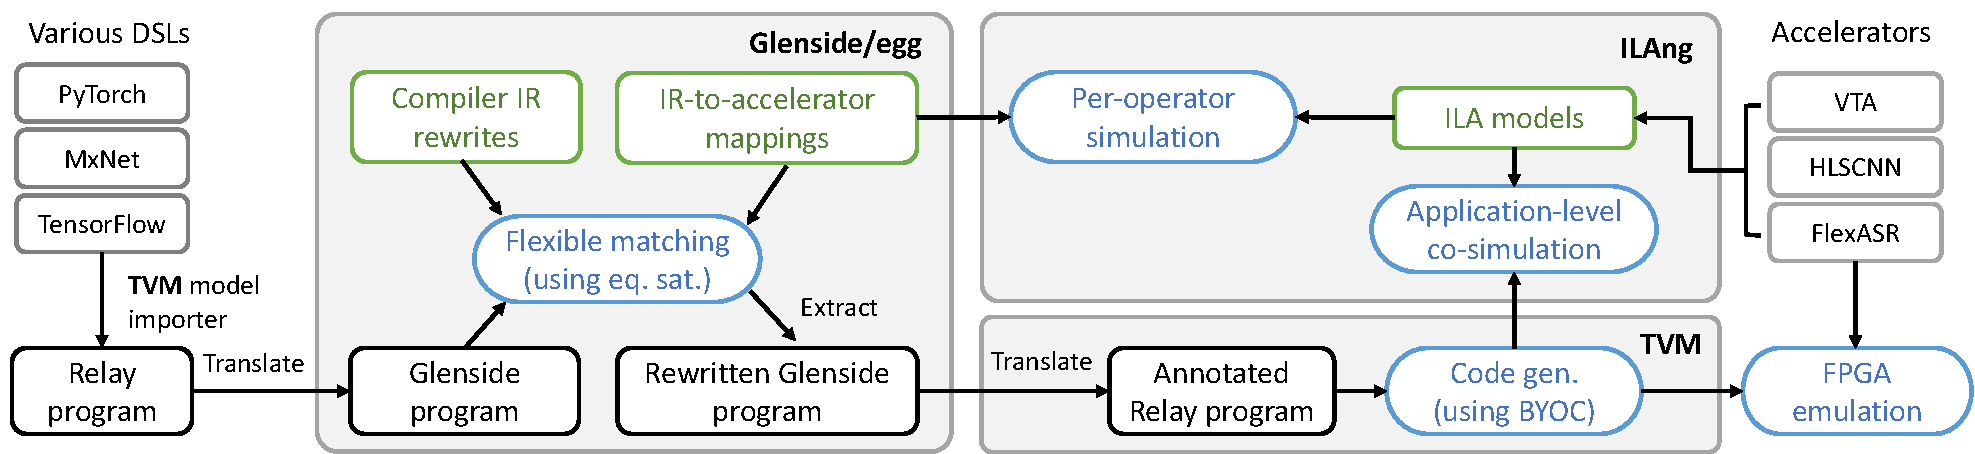
\includegraphics[width=\textwidth]{assets/3la-diagram.pdf}
    \caption{
    \hl{not quite sure where this goes}
This figure first appeared
  in Huang et.~al.~\cite{huang2024application}.
Diagram of the 3LA prototype's flow.
Note that only the ``Glenside/egg''
  portion of 3LA
  is considered a contribution
  of this dissertation;
  for more information on the other components,
  please see the original paper.
}
    \label{fig:3la-diagram}
\end{figure}

3LA solves two major problems:
  first, generating simulators
  for hardware
  is difficult
  and time consuming.
Second, even given a simulator
  for your design,
  it is then difficult
  to run full applications
  on the simulator.
The first contribution
  of 3LA
  we do not consider
  a contribution of this dissertation;
  please refer to the dissertation
  of Bo-Yuan Huang~\cite{huang2022instruction}.

However,
  the second contribution of 3LA
  results directly from contributions
  of this thesis.
One of the challenges
  that 3LA solves:
  compiling to custom hardware is hard.
This is where I was able
  apply my dissertation.
We developed a language
  called \g
  which allowed for the application
  of equality saturation


%% GLENSIDE INTRO

Adding accelerator support to
  an existing compiler typically
  uses custom pattern matching to
  map expensive tensor operations
  from applications down to
  accelerator invocations~\cite{
    yang2020interstellar, byoc}.
Pattern matching often additionally relies on
  various other transformations
  to canonicalize intermediate representations (IRs)
  %~\cite{??}
  and massage data layouts into
  formats matching accelerator requirements~\cite{nvidia2020nhwc}.
Even with these changes,
  users may need to manually modify their application to
  help the compiler discover opportunities
  for dispatching operations to accelerators, 
  such as by changing data types or unrolling loops.
\hl{
These modifications may be especially
  untenable
  for hardware developers,
  who may not have practical experience
  with the workloads
  and toolchains. 
(something tying it in to new combined intro)
}
    
In principle, term rewriting techniques~\cite{baader1998term}
  should be able to facilitate many of
  these transformation and mapping tasks
  within a compiler.
Halide and TVM already rely
  on extensive rewrite systems for
  optimizing scalar computations and
  simplifying loop bounds in order to
  support further downstream optimizations~\cite{newcomb2020halide-rewrite,
  hagedorn2020func-high-perf}.

Unfortunately, existing IRs in compilers for
  array/tensor programming DSLs tend to
  present abstraction and granularity mismatches
  that hamper term rewriting approaches.
Term rewriting is most easily applied in
  \textit{pure} (side effect--free) IRs
  that support equational reasoning.
At the same time,
  mapping to accelerators requires considering
  low-level hardware details like data layout.
Existing pure IRs for ML frameworks are used
  primarily for high-level transformations
  (e.g., type elaboration and inlining)
  and do not expose low-level data layout details~\cite{relay}.
On the other hand,
  IRs used for crucial lower-level optimizations like
  operator fusion must support
  precise reasoning about memory use,
  and therefore are typically impure,
  hampering term rewriting.% approaches.

To help mitigate such impedance mismatches,
  we present \textit{\g},\footnote{Publicly available at \url{https://github.com/gussmith23/glenside}.}
  a pure tensor program IR
  that enables hardware-level term rewriting.
\g is based on a simple
  \textit{access pattern} abstraction that
  supports expressing and reasoning about
  data layout transformations via
  syntactic rewrite rules.
  \begin{figure}
    \centering
    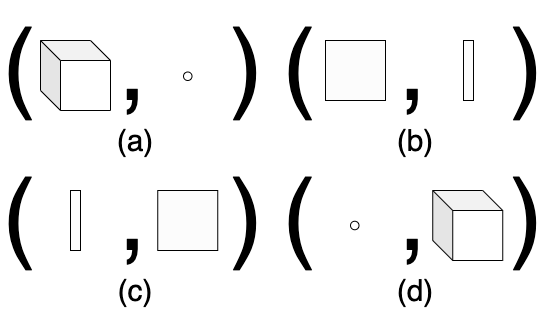
\includegraphics[width=.6\linewidth]{glenside/access-pattern-examples-2x2.png}
    \caption{
      Four access patterns,
        representing different ways
        a
        tensor program
        (or \textit{kernel})
        might access
        the same 3D tensor. 
      For example, (c) represents
        accessing a 3D tensor as
        a vector of 2D matrices.}
    \label{fig:access-pattern-examples}
    \vspace{-1em}
\end{figure}
When combined with standard arithmetic rewrites
  for per-tensor-element computations,
  access patterns enable implementing complex
  transformations for accelerator support as
  compositions of simple rewrites.

Tensors are traditionally characterized
  by their \textit{shape},
  an $n$-tuple 
  %in $\mathbb{N}^n$
  of positive integers
  indicating the size of each
  of a tensor's dimensions.
  % , e.g., $(x, y, z)$ for a 3D tensor.
Access patterns instead characterize
  each tensor with two shapes, e.g.,
  \accesspatternshape{x}{y, z}, separating
  the dimensions which are \textit{iterated over} from
  the dimensions which are \textit{computed on.}
Figure~\ref{fig:access-pattern-examples}(c)
  depicts an example where a 3D tensor's
  first dimension is iterated over and
  some computation applied to each
  corresponding 2D matrix.

\g \hl{
 plays a crucial role in the 3LA framework.
}
We demonstrate how \g
  enables implementing representative
  hardware-level transformation via term rewriting,
  including mapping computations
  to systolic arrays~\cite{jouppi2017tpu}
  (a common hardware module in ML accelerators)
  and automatically discovering the
  \tcd{im2col} data layout transformation~\cite{im2col},
  which enables mapping 2D convolutions
  to matrix multiplication hardware.
In particular,
  by employing \textit{equality saturation}~\cite{willsey2021egg},
  these transformations ``fall out for free''
  (i.e., without any carefully crafted
  rewrite orderings~\cite{phase-ordering}),
  from a handful of general rewrites concerning tensor
  transposition, Cartesian product, dot product, etc.,
  expressed in terms of access patterns.


\hl{move this to glenside chapter?}
 The rest of this chapter is organized as follows:
Section~\hl{todo} provides background
  and briefly surveys closely related work.
Section~\ref{sec:matmul} motivates
  \g via a running example exploring
  pure matrix multiplication.
Section~\ref{sec:glenside} details the
  design and implementation of \g.

%% END GLENSIDE INTRO

Skipping over the comparisons with related work.
If we include anything, it should be something
  from the Task 1 paraagraph, re comparison with Exo, MLIR, etc.

Should take something from "detailed comparison
  with closely related tools".

Background. Can probably skip 2.1.

Probably want 2.2. But maybe should just be the Glenside chapter.

But then we need to find a way
  to lead into the Glenside intro.

Would be great to set up this chapter
  so that it ends with a very clear statement
  of what we need our language to do.
Then the Glenside chapter can do those things.
But we also need to make sure
  we tie it back to the thesis.


  To summarize, the contributions of this chapter include:
\begin{itemize}
\item \textit{Access patterns},
  a tensor representation that employs a
  simple, extended tensor shape type to
  distinguish iteration and computation dimensions

\item The \g IR,
  a pure compiler IR that facilitates 
  term rewriting to enable support for
  specialized accelerators
  
\item A library of generic rewrites over \g programs
  
% \item Case studies demonstrating how
%   \g enables automatically discovering
%   key transformations for mapping
%   applications to custom accelerators
%   via equality saturation with the
%   \tcd{egg}~\cite{willsey2021egg} library.
\end{itemize}


% 3LA methodology needs flexible matching.
\section{3LA Methodology}


We now give a description
  of the structure
  of the 3LA methodology
% \begin{abstract}

% Tensor kernels in machine learning (ML)
%   often correspond to pure mathematical expressions,
%   making term rewriting an attractive strategy
%   for optimization and mapping to specialized hardware accelerators.
% %   ---%
% %   especially given recent progress in equality saturation.
% However,
%   existing ML intermediate representations (IRs)
%   tend to either be \textit{pure but high-level},
%   making low-level rewrites
%   to hardware targets inexpressible,
%   or \textit{low-level but impure},
%   hampering the use of term rewriting altogether.
% %   leaving no suitable IR
% %   for term rewriting
% %   over low-level tensor kernels.

% This paper introduces \g,
%   a pure IR whose core abstraction---%
%   the \textit{access pattern}---%
%   enables
%   low-level,
%   layout-aware,
%   hardware-centric
%   program rewrites.
% We demonstrate how term rewriting
%   in \g
%   can be used to 
%   map program fragments
%   to hardware accelerator invocations
%   and
%   automatically discover
%   classic data layout transformations
%   like \tcd{im2col}.
% % Hm... not capturing this idea at the moment:
% %  that facilitate hardware--software mapping
% %  but previously required explicit manual implementation.
% \g establishes a new foundation for
%   exploring further term rewriting techniques
%   in optimizing low-level tensor programs.
% %  \hl{todo we don't ever explain hardware--software programs}



% \end{abstract}

\chapter{Glenside}
\label{sec:part1-glenside}

\textit{This chapter is derived from Smith et.~al.~\cite{smith2021pure}.}

\section{Introduction}

\hl{should this stuff be moved up to 3LA?}

Machine learning (ML) and other
  high-performance computing (HPC)
  applications increasingly rely on
  specialized hardware accelerators to
  provide speed and energy efficiency~\cite{jouppi2017tpu, krizhevsky2012conv, reuther2019survey}.
This trend has highlighted the need
  for flexible accelerator support
  in domain-specific compilers like
  Halide~\cite{halide},
  TVM~\cite{chen2018tvm},
  TensorFlow/MLIR~\cite{tensorflow, mlir}, and
  PyTorch~\cite{pytorch}.

Adding accelerator support to
  an existing compiler typically
  uses custom pattern matching to
  map expensive tensor operations
  from applications down to
  accelerator invocations~\cite{
    yang2020interstellar, byoc}.
Pattern matching often additionally relies on
  various other transformations
  to canonicalize intermediate representations (IRs)
  %~\cite{??}
  and massage data layouts into
  formats matching accelerator requirements~\cite{nvidia2020nhwc}.
Even with these changes,
  users may need to manually modify their application to
  help the compiler discover opportunities
  for dispatching operations to accelerators, 
  such as by changing data types or unrolling loops.
    
In principle, term rewriting techniques~\cite{baader1998term}
  should be able to facilitate many of
  these transformation and mapping tasks
  within a compiler.
Halide and TVM already rely
  on extensive rewrite systems for
  optimizing scalar computations and
  simplifying loop bounds in order to
  support further downstream optimizations~\cite{newcomb2020halide-rewrite,
  hagedorn2020func-high-perf}.

Unfortunately, existing IRs in compilers for
  array/tensor programming DSLs tend to
  present abstraction and granularity mismatches
  that hamper term rewriting approaches.
Term rewriting is most easily applied in
  \textit{pure} (side effect--free) IRs
  that support equational reasoning.
At the same time,
  mapping to accelerators requires considering
  low-level hardware details like data layout.
Existing pure IRs for ML frameworks are used
  primarily for high-level transformations
  (e.g., type elaboration and inlining)
  and do not expose low-level data layout details~\cite{relay}.
On the other hand,
  IRs used for crucial lower-level optimizations like
  operator fusion must support
  precise reasoning about memory use,
  and therefore are typically impure,
  hampering term rewriting.% approaches.

To help mitigate such impedance mismatches,
  we present \textit{\g},\footnote{Publicly available at \url{https://github.com/gussmith23/glenside}.}
  a pure tensor program IR
  that enables hardware-level term rewriting.
\g is based on a simple
  \textit{access pattern} abstraction that
  supports expressing and reasoning about
  data layout transformations via
  syntactic rewrite rules.
% We moved this figure elsewhere in the thesis
%   \begin{wrapfigure}{r}{.5\textwidth}
%     \centering
%     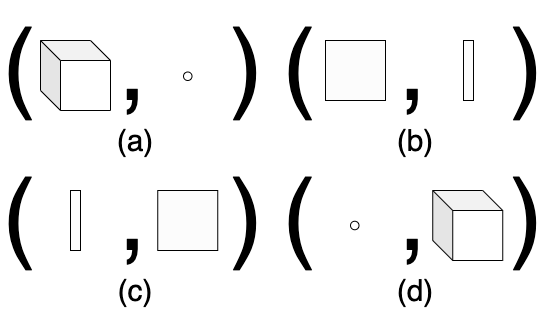
\includegraphics[width=.9\linewidth]{glenside/access-pattern-examples-2x2.png}
%     \caption{
%       Four access patterns,
%         representing different ways
%         a
%         tensor program
%         (or \textit{kernel})
%         might access
%         the same 3D tensor. 
%       For example, (c) represents
%         accessing a 3D tensor as
%         a vector of 2D matrices.}
%     \label{fig:access-pattern-examples}
%     \vspace{-1em}
% \end{wrapfigure}
When combined with standard arithmetic rewrites
  for per-tensor-element computations,
  access patterns enable implementing complex
  transformations for accelerator support as
  compositions of simple rewrites.

Tensors are traditionally characterized
  by their \textit{shape},
  an $n$-tuple 
  %in $\mathbb{N}^n$
  of positive integers
  indicating the size of each
  of a tensor's dimensions.
  % , e.g., $(x, y, z)$ for a 3D tensor.
Access patterns instead characterize
  each tensor with two shapes, e.g.,
  \accesspatternshape{x}{y, z}, separating
  the dimensions which are \textit{iterated over} from
  the dimensions which are \textit{computed on.}
Figure~\ref{fig:access-pattern-examples}(c)
  depicts an example where a 3D tensor's
  first dimension is iterated over and
  some computation applied to each
  corresponding 2D matrix.

We demonstrate how \g
  enables implementing representative
  hardware-level transformation via term rewriting,
  including mapping computations
  to systolic arrays~\cite{jouppi2017tpu}
  (a common hardware module in ML accelerators)
  and automatically discovering the
  \tcd{im2col} data layout transformation~\cite{im2col},
  which enables mapping 2D convolutions
  to matrix multiplication hardware.
In particular,
  by employing \textit{equality saturation}~\cite{willsey2021egg},
  these transformations ``fall out for free''
  (i.e., without any carefully crafted
  rewrite orderings~\cite{phase-ordering}),
  from a handful of general rewrites concerning tensor
  transposition, Cartesian product, dot product, etc.,
  expressed in terms of access patterns.

To summarize, the contributions of this chapter include:
\begin{itemize}
\item \textit{Access patterns},
  a tensor representation that employs a
  simple, extended tensor shape type to
  distinguish iteration and computation dimensions

\item The \g IR,
  a pure compiler IR that facilitates 
  term rewriting to enable support for
  specialized accelerators
  
\item A library of generic rewrites over \g programs
  
% \item Case studies demonstrating how
%   \g enables automatically discovering
%   key transformations for mapping
%   applications to custom accelerators
%   via equality saturation with the
%   \tcd{egg}~\cite{willsey2021egg} library.
\end{itemize}

\hl{i moved related work, so probably need to rework this}
The rest of this chapter is organized as follows:
Section~\hl{todo} provides background
  and briefly surveys closely related work.
Section~\hl{todo} motivates
  \g via a running example exploring
  pure matrix multiplication.
Section~\hl{todo} details the
  design and implementation of \g.


\section{From Pure \texttt{matMul} to IR Design Goals}
\label{sec:matmul}

% Many ML and HPC workloads are dominated by
%   evaluating compositions of tensor algebra operators
%   which, at a high level, correspond to
%   pure mathematical expressions.
% This make functional programming techniques attractive,
%   but requires careful design to ensure that
%   nested operators remain compositional with
%   respect to their output shapes.
% To highlight these design constraints and
%   motivate access patterns,
%   in this section we walk through a simple
%   matrix multiplication example to
%   illustrate the pitfalls that access patterns in \g
%   help mitigate.
  
Applying functional techniques
  and term rewriting to tensor IRs
  requires careful design.
For example,
  we must ensure that operators be compositional
  with respect to tensor shapes
  and that the representation support
  generic rules within the
  target rewrite engine.
To highlight such constraints and
  motivate access patterns in \g,
  this section illustrates potential pitfalls
  with a simple matrix multiplication example.

\subsection{Pure Matrix Multiplication}
\label{subsec:pure-matmul}

We write
  \tcd{f64} for the type of 64-bit floats and
  \tcd{[A]} for vectors over type \tcd{A}.
Using this notation, we can specify operators like
  dot product and 2D matrix transpose as:
\begin{align*}
    \mcd{dotProd} &
    \mcd{ : [f64] * [f64] -> f64} \\
    \mcd{trans2} &
    \mcd{ : [[f64]] -> [[f64]]}
\end{align*} 

% \begin{itemize}[leftmargin=*]
% \item
%   \tcd{[[f64]]} as the type of 2D matrices

% \item
%   \tcd{trans2 : [[f64]] -> [[f64]]} as matrix transpose

% \item 
%   \tcd{dotProd : [f64] * [f64] -> [f64]} 
%   as dot product
% \end{itemize}

%   so that, e.g.,
%   \tcd{[f64] * [f64] -> [f64]} represents
%   the type of a dot product operator \tcd{dotProd},
%   \tcd{[[f64]]} represents the type of
%   2D matrices of 64-bit floats, and
%   \tcd{[f64] * [f64] -> [f64]} represents
%   the type of a dot product operator.

% \noindent
% Assuming row-major layout,
%   implementing 2D matrix multiplication
%   on inputs \tcd{P} and \tcd{Q},
%   requires computing an output matrix
%   \tcd{R} such that:
% $$
%   \mcd{R[i][j] = dotProd(P[i],\, trans2(Q)[j])}
% $$

\noindent
Implementing 2D matrix multiplication
  on inputs $P$ and $Q$ requires computing
  an output matrix $R$ where
  $R_{ij} = \Sigma_k P_{ik} \, Q_{kj}
          =  P_i \cdot Q^{T}_{j}$. %\mcd{dotProd}(P_i, Q^{T}_{j}).$ 
The need to compute \tcd{dotProd} for every pair
  of a row from $P$ and a column from $Q$
  suggests map and Cartesian product operators
  which we might specify with:
\begin{align*}
    \mcd{map} &
    \mcd{ : (A -> B) * [A] -> [B]} \\
    \mcd{cartProd} &
    \mcd{ : [A] * [B] -> [A * B]}
\end{align*}
Naively, we can almost implement matrix multiplication as:
{\color{red} \begin{align*}
  & \mcd{matMul(P, Q) :=} \\
  & \;\;\;\;\; \mcd{map(dotProd, cartProd(P, trans2(Q)))}
\end{align*} }
% {\color{red} $$
%   \mcd{map(dotProd, cartProd(P, trans2(Q)))}
% $$ }
However, the result type will have been
  flattened to just {\color{red}\tcd{[f64]}},
  making it impossible to compose with other matrix
  operators that expect \tcd{[[f64]]} inputs.

Our first problem is that
  the \tcd{cartProd} specification above
  ``forgets'' the shape of its arguments.
We could change this specification to
  arrange the output as a matrix:
  % according to  the positions of its argument's indices
$$
  \mcd{cartProd2D : [A] * [B] -> [[A * B]]}
$$
But this result type prevents
  directly mapping \tcd{dotProd}.\footnote{
    This simple type does not specify how
    \tcd{cartProd2D} orders its output
    relative to its input vectors.
    We assume the order
    expected for matrix multiplication.}
Now the problem is that \tcd{map}
  only applies a computation by iterating
  over the first (outermost) dimension of a tensor.
If we specialize \tcd{map} to iterate
  over the second dimension:
$$
  \mcd{mapAt2 : (A -> B) * [[A]] -> [[B]]}
$$
then we can implement a compositional
  \tcd{matMul} operator that correctly produces
  results of type \tcd{[[f64]]} as:
\begin{align*}
  & \mcd{matMul(P, Q) :=} \\
  & \;\;\;\;\; \mcd{mapAt2(dotProd, cartProd2D(P, trans2(Q)))}
\end{align*}

While this gets us close
  to our goal of a pure, functional
  IR for tensor programs,
  as we'll see,
  this style also has its issues.

\subsection{\g Design Constraints and Goals}

This style of pure, higher-order functional
  program representation enables
  term rewriting and equational reasoning
  via rules like:
\begin{align*}
  \mcd{dotProd(P, Q)}
    & \leftrightsquigarrow
      \mcd{dotProd(Q, P)} \\[2pt]
  \mcd{trans2(trans2(P))}
    & \leftrightsquigarrow
      P \\[2pt]
  \mcd{map(f, map(g, P))}
    & \leftrightsquigarrow
      \mcd{map(f$\,\circ\,$g, P)} \\[2pt]
  \mcd{mapAt2(f, trans2(P))}
    & \leftrightsquigarrow
      \mcd{trans2(mapAt2(f, P))} % \\[2pt]
\end{align*}

% \footnote{
%     In these rules, we assume \tcd{reduce}
%     (``\tcd{fold}'') requires its first argument
%     to be an associative and commutative operator.}
%   \mcd{reduce(f, trans2(P))}
%     & \leftrightsquigarrow
%       \mcd{reduce(f, P)} \\[2pt]
%   \mcd{reduce(f, cartProd(P, Q))}
%     & \leftrightsquigarrow \\
%       \omit\rlap{\tcd{\hspace{0.5in}
%          reduce(f$\,\circ\,$swap, cartProd(Q, P))}}

However, some of these rules depend on the
  shapes of dimension-specific operators aligning.
What happens when we need to support
  higher-dimensional tensors?
Without a mechanism to abstract
  which dimensions of a tensor
  are being iterated as opposed to computed over,
  we would have to generate versions of
  each rule for every combination of dimensions.
Worse, these problems
  do not only affect rewrite rules;
  they also lead to code blowup just to
  specify all the variants of tensor kernels
  that arise in practice---%
  e.g.~we would eventually need
  \texttt{mapAt3}, \texttt{mapAt4},
  and so on.

One strategy to address these challenges is
  adding support for anonymous functions (``lambdas''),
  currying, and closures to the 
  tensor program representation.
These features can provide sufficient
  flexibility to handle shape alignment
  issues that otherwise may require
  dimension-specific operators like
  \tcd{cartProd2D} and \tcd{mapAt2} above.
\hl{maybe make specific references here?}
For example, given curried versions
  of \tcd{dotProd} and \tcd{map},
  we could have used such features
  to implement a curried \tcd{matMul} as:
\begin{align*}
  & \mcd{matMul' P Q :=} \\
  & \;\; \mcd{ \
      map' ($\boldsymbol\lambda\,$r =>\
        map' (dotProd' r) (trans2 Q)) P}
\end{align*}
Alternatively, some IRs rely on index notation
  for even pithier implementations like:
$$
  \mcd{matMul(P,Q)[i,j] := dotProd(P[i], trans2(Q)[j])}
$$

Unfortunately, these approaches all rely on some
  form of \textit{name binding} which can
  significantly complicate term rewriting.
Rewriting under binders,
  whether explicitly in the form of lambdas
  or implicitly with index notation,
  requires additionally analyzing the
  potential \textit{contexts}
  (what names are bound to)
  of every subexpression.
While it is still technically possible to
  apply state-of-the-art rewrite engines
  like \tcd{egg}~\cite{willsey2021egg}
  via explicit variable substitution rules and
  free variable analyses,
  we have found the additional complexity
  and rewrite search space blow up
  substantially eliminate the potential advantages
  of term rewriting in such IR designs.

All the above constraints inform \g's key design goal:
  providing an IR that flexibly supports specifying and
  composing higher-order tensor operators\footnote{
    As \tcd{map} and \tcd{mapAt2} in 
    Section~\ref{subsec:pure-matmul} illustrate,
    an IR can support higher-order operators without
    necessarily providing lambdas, currying, or closures.}
  over arbitrary dimensions while still enabling
  high-performance term rewriting techniques
  like equality saturation.
In the rest of this paper,
  we show how \textit{access patterns} enable achieving
  these goals with a focus on applications to
  mapping application fragments down to
  specialized hardware accelerators.

%\hl{
%Need to be explicit somewhere that access patterns,
%especially things like cartesian product,
%can just be for specification -- you 
%do not necessarily have
%to materialize everything.}

%\hl{(Probably worth saying that rewrite systems need pure IRs. Maybe consider a phrasing like this --Steve) ``However, rewrite systems are generally defined over pure languages---how will we represent matrix multiplication in a pure IR?''}
  
%{\color{red} \noindent\rule{8.5cm}{10pt}}


% {\color{red} \begin{align*}
%     & \mcd{matMul(A, B) :=} \\
%     & \;\;\;\; \mcd{map(dotProd, cartProd(A, trans2(B)))}
% \end{align*} }

% $$ 
% {\color{red}
%   \mcd{cartProd : [f64] * [f64] -> [f64 * f64]}
% }
% $$




% %To understand
% %  the genesis
% %  of access patterns,
% %  let's walk through
% %  an example.
% Let us consider an example
%   to motivate 
%   the access pattern representation.
% %Imagine 
% %  we'd like to build
% %  a simple term rewriting system
% %  to map matrix multiplications
% %  to an accelerator.
% %  we've built.
% Suppose we would like
%   to use 
%   a simple term rewriting system 
%   to map matrix multiplications
%   to an accelerator.
% Before we can start building rewrites,
%   we need to
%   represent our programs of interest---%
%   beginning with matrix multiplication---%
%   in a pure IR.

% Recall 
%   the matrix multiplication
%   algorithm:
%   given two two-dimensional tensors
%   $a$ and $b$
%   with shapes
%   $(M, N)$
%   and
%   $(N, O)$,
%   respectively,
%   we take the dot product
%   of every row of $a$
%   with every column of $b$,
%   to produce a new tensor
%   with shape $(M, O)$.
% The English description
%   of the algorithm
%   immediately suggests
%   a pure
%   representation,
%   shown in
%   Figure \ref{fig:matmul-haskell} left.
% Assume
%   \texttt{a}
%   and \texttt{b}
%   are two-dimensional tensors
%   with
%   some tensor type.
% Here,
%   we use a simple implementation
%   for our tensor type:
%   lists of lists,
%   \texttt{[[f64]]}.
% \texttt{(rows a)}
%   and \texttt{(cols b)}
%   produce lists
%   of the rows of \texttt{a}
%   and the columns of \texttt{b},
%   respectively.
% Using our nested-lists
%   tensor type,
%   \texttt{rows}
%   is simply
%   the identity function,
%   and \texttt{cols}
%   is a transpose function.
% \texttt{cartProd}
%   returns every element 
%   of the first list
%   paired with every element
%   of the second list;
%   in this case, 
%   every row of \texttt{a}
%   paired with
%   every column of \texttt{b}.
% \texttt{dotProduct}
%   computes the dot product
%   of two vectors.
% Putting it all together,
%   we \texttt{map}
%   the \texttt{dotProduct}
%   over our row--column pairs,
%   producing a result
%   with type
%   \texttt{[f64]}.
  
% Something doesn't seem right about this.
% The result
%   of multiplying
%   two two-dimensional tensors
%   should be a 
%   two-dimensional tensor,
%   not a one-dimensional list.
% Our program
%   computes the right values,
%   but it loses
%  a key piece of information:
%   the shape
%   of the resulting tensor.
% % I'm not actually sure we need to explain why shape is important.
% %Preserving
% %  shape information
% %  in a tensor-based
% %  program
% %  is essential.
% %Shape
% %  is the de facto way
% %  in which type
% %  information
% %  is conveyed
% %  in many tensor-based programs.
% %Perhaps
% %  the most common example
% %  is in activation layouts:
% %  an activation layout
% %  of \texttt{NCHW},
% %  for example,
% %  conveys which dimension
% %  is the batch dimension
% %  (\texttt{N}),
% %  which dimension is the channel
% %  dimension
% %  (\texttt{C}),
% %  and which dimensions
% %  are the spatial dimensions
% %  (\texttt{H} and
% %    \texttt{W}),
% %  and their order.
% Let's understand
%   where
%   the shape information
%   was lost.
% Both
%   \texttt{rows}
%   and
%   \texttt{cols}
%   preserve shape information,
%   which we can see
%   from their type,
%   \texttt{[[f64]] -> [[f64]]}.
% What about
%   \texttt{cartProd}?
% Its type signature
%   is
%   \texttt{[f64] -> [f64] -> [(f64, f64)]};
%   given two lists,
%   it returns a list of tuples.
% This new list
%   is of length
%   \texttt{length l0 * length l1}
%   for lists
%   \texttt{l0} and \texttt{l1}.
% In our example,
%   \texttt{rows a}
%   is a list of length $M$
%   of lists of length $N$,
%   and \texttt{cols b}
%   is a list of length $O$
%   of lists of length $N$.
% Thus,
%   \texttt{cartProd}
%   produces a list of length
%   $M \cdot O$
%   of 2-tuples
%   containing lists of length $N$.
% By the time
%   we map
%   \texttt{dotProduct}
%   over this list,
%   the shape information
%   has already been lost;
%   \texttt{dotProduct}
%   simply produces
%   another list
%   of length $M \cdot O$,
%   but with scalar values.
% It would seem
%   shape information
%   is lost
%   by \texttt{cartProd}.

% What
%   were we expecting
%   the result 
%   of \texttt{cartProd}
%   to be?
% We expect
%   the result of
%   the entire \texttt{map} expression
%   to be a tensor
%   with shape
%   $(M, O)$;
%   that is,
%   the outermost dimensions
%   of the original two inputs
%   ($M$ and $O$, respectively)
%   need to be preserved
%   \textit{separately,}
%   rather than
%   being \textit{flattened}
%   into a single dimension
%   of length $M \cdot O$.
% %Thus,
% %  the result of
% %  \texttt{cartProd}
% %  should presumably
% %  have a shape like
% %  $(M, O, \dots)$,
% %  rather than
% %  $(M*O, \dots)$.
% This brings us
%   to our first core obstacle:
%   we are using
%   the
%   one-dimensional list
%   semantics
%   of common functions
%   such as
%   \texttt{cartProd},
%   when
%   we need more complex semantics
%   for our more complex
%   tensor type.
  
% As a first pass
%   at this obstacle,
%   we can redefine
%   \texttt{cartProd}
%   to preserve
%   shape information.
% Its type signature
%   will change
%   from
%   \texttt{[f64] -> [f64] -> [(f64, f64)]}
%   to
%   \texttt{[f64] -> [f64] -> [[(f64, f64)]]}.
% That is,
%   rather than producing
%   a single list
%   whose length is a product
%   of the input lists' lengths,
%   we will produce a list of lists,
%   or a two-dimensional tensor.
% This
%   preserves
%   our shape information.
  
% Now, though,
%   we are presented
%   with another problem;
%   how should \texttt{map}
%   work
%   over our tensor representation?
% Currently,
%   \texttt{map}'s type
%   is 
%   \texttt{(f64 -> f64) -> [f64] -> [f64]};
%   thus,
%   it will attempt to map
%   our uncurried
%   \texttt{dotProduct}
%   over only 
%   the \textit{outermost}
%   dimension
%   of the result of 
%   \texttt{cartProd}.
% Not only
%   is this not what we want---%
%   it is also 
%   a type error.
% By preserving
%   the shape information
%   through
%   \texttt{cartProd},
%   we have necessitated
%   a more complex
%   implementation
%   of \texttt{map}.
% Specifically,
%   \texttt{map}
%   needs to understand
%   which dimensions
%   of the input tensor
%   should be considered the
%   ``list'' dimensions,
%   unaffected by the map,
%   and which dimensions
%   should be considered
%   the ``item'' dimensions,
%   which represent
%   the data structure
%   being passed in
%   to the function.
% In this case,
%   we want
%   \texttt{map}
%   to map the function
%   over the tuples
%   contained in the second
%   level
%   of lists.
% Figure \ref{fig:matmul-haskell} right
%   shows
%   our updated 
%   matrix multiplication,
%   using a new function,
%   \texttt{tensorMap2},
%   which treats
%   tensor dimensions
%   0 and 1
%   as ``list'' dimensions
%   and maps a function
%   over dimension 2
%   and above.

% With our change to
%   \texttt{cartProd}
%   and our new version
%   of \texttt{map},
%   we finally have
%   a functional representation
%   of matrix multiplication.
% Using this representation,
%   we can start writing rewrite rules
%   for our hardware accelerator,
%   in terms of
%   \tcd{tensorMap2},
%   \tcd{dotProduct}, and
%   \tcd{cartProd}.
% However,
%   these operators
%   are defined
%   for our specific
%   two-dimensional
%   usecase,
%   and thus, the rewrite would be brittle;
%   if $a$ or $b$
%   had more dimensions,
%   we would again
%   need to redefine
%   \texttt{map},
%   \texttt{cartProd},
%   and our rewrite as a whole.
  
% \texttt{cartProd}
%   and
%   \texttt{tensorMap2}
%   are conveying
%   which dimensions
%   of the input tensors
%   are being \textit{iterated over}
%   and which are
%   being \textit{computed on}.
% But instead
%   of conveying
%   this information
%   in these functions'
%   types,
%   it
%   could instead
%   be conveyed 
%   by the type
%   of the tensor itself.
% This is the core insight
%   of access patterns,
%   which we will now describe.
  
\section{\g}
\label{sec:glenside}
  
% Trying to get this to end up on the right page...
\begin{table*}
    \centering
    \caption{\g's access pattern transformers. \hl{formatting}}
    \label{tab:access-pattern-transformers}
    \begin{tabularx}{\linewidth}{lXX}
    Transformer 
    & Input(s)
    & Output Shape  \\
    \hline
    
    %%%%%% ACCESS
    \texttt{access} 
    &
    \accesspatternshape{a_0,\dots}{\dots, a_n}
    and non-negative integer $i$
    & 
  \accesspatternshape
  {a_0, \dots, a_{i-1}}{a_i,\dots, a_n}
    \\
    
    %%%%% TRANSPOSE
    \texttt{transpose} &
    \accesspatternshape{a_0,\dots}{\dots, a_n},  $\ell$ (a permutation of $(0, \dots, n-1)$) &
    \accesspatternshape{a_{\ell_0},\dots}{\dots, a_{\ell_n}}
    \\
    
    \texttt{cartProd} 
    &
    \accesspatternshape{a_0,\dots, a_n}{c_0, \dots, c_p},  \accesspatternshape{b_0,\dots, b_m}{c_0, \dots, c_p}
    & 
  \accesspatternshape
  {a_0, \dots, a_n, b_0,\dots, b_m}
  {2, c_0, \dots, c_p}
    \\
    %...implementing the rows-by-columns data reading pattern used in matrix multiplication; implementing the filter--window pairing in \ctd{} \\
    
    %%%% WINDOWS
    \texttt{windows} 
    &
    \accesspatternshape{a_0, \dots, a_m}{b_0, \dots, b_n}, \newline
    window shape $(w_0, \dots, w_n)$,
    strides $(s_0, \dots, s_n)$
    &
    \accesspatternshape{a_0, \ldots, a_m, b'_0, \dots, b'_n}{w_0, \dots, w_n},\newline
    where $b'_i = \lceil (b_i - (k_i - 1)) / s_i \rceil $\\
    
    %%%% SLICE
    \texttt{slice} &
    \accesspatternshape{a_0, \dots }{\dots, a_n}, \newline
    dimension index $d$, bounds $[l, h)$
    &
    \accesspatternshape{a'_0, \dots }{\dots, a'_n} \newline
    with $a'_i = a_i$ except $a'_d = h - l$
    \\
    %...accessing a subset of a tensor \\
    
    \texttt{squeeze} &
    \accesspatternshape{a_0, \dots }{\dots, a_n}, index $d$ where $a_d = 1$
    &
    \accesspatternshape{a_0, \dots }{\dots, a_n} with $a_d$ removed
    \\
    
    \texttt{flatten} &
    \accesspatternshape{a_0,\dots,a_m}{b_0,\dots,b_n} &
    \accesspatternshape{a_0 \cdots a_m}{b_0 \cdots b_n} \\
    
    \texttt{reshape} &
    \accesspatternshape{a_0,\dots,a_m}{b_0,\dots,b_n},\newline
    access pattern shape literal
    \accesspatternshape{c_0,\dots,c_p}{d_0,\dots,d_q}&
    
    \accesspatternshape{c_0,\dots,c_p}{d_0,\dots,d_q},\newline
    if $a_0 \cdots a_m = c_0 \cdots c_p$
    and $b_0 \cdots b_n = d_0 \cdots d_q$\\
    
    %%% PAIR
    \texttt{pair}&
    two access patterns of shape
  \accesspatternshape
  {a_0, \dots}{\dots, a_n} &
  \accesspatternshape
  {a_0, \dots}{2, \dots, a_n}
    \\
    
    \end{tabularx}
\end{table*}

%\hl{Move up resolution of section 3 to beginning of section 4}

%\hl{max: do a bigger bomb drop. what have we done before we compute dot product? we've set up a complex system of accessing, which is completely separate from the computation that we're doing}

%\hl{the interesting thing is that these kernels end up looking very similar when you phrase them in glenside}

%\hl{need to say that we're solving the problem we set up}

%\hl{see, we've done what we said we're going to do}

This section details \g's implementation,
  focusing on its core abstraction,
  \textit{access patterns}.
We use Section~\ref{sec:matmul}'s
  matrix multiplication as a
  running example throughout.
  %beginning
  %with the definition
  %of access patterns,
  %then ways we can combine access patterns,
  %and finally,
  %describing how we compute over access %patterns.
%To illustrate,
   %we will progressively convert
   %the matrix multiplication example
   %from Section~\ref{sec:matmul}
   %to our final \g implementation.
  

\subsection{Access Patterns}

% Access patterns
%   encode a common trope
%   in tensor programs
%   in which
%   some of the dimensions of a tensor
%   are \textit{iterated over}/\textit{accessed}
%   while others are
%   \textit{computed on.}

Access patterns encode common
  tensor IR patterns where
  some tensor dimensions
  are \textit{iterated over} (accessed)
  while others are \textit{computed on}.\footnote{
    This is similar to NumPy's concept of \textit{universal functions.}}
Section~\ref{sec:matmul}'s \tcd{matMul} example
  \textit{iterates over} dimension 0 of input $P$,
  while \textit{computing on} dimension 1,
  effectively viewing $P$ as a 1D vector of 1D vectors.

Access patterns are specified by their \textit{shape} ---
  a pair of tuples of positive integers $(S_A, S_C)$.
An access pattern of shape $(S_A, S_C)$ is, in turn, a
  tensor $T$ whose shape is given by the
  concatenation of the access pattern shape tuples
  $S_A \,\mcd{++}\, S_C$; we refer to
  $S_A$ and $S_C$ as the \textit{access} and
  \textit{compute}
  dimensions of $T$, respectively.

Access patterns represent the view of an
  $(|S_A| + |S_C|)$--dimensional tensor
  as a tensor of shape $S_A$,
  each of whose elements has shape $S_C$.
For an access pattern $T$ of shape $(S_A, S_C)$
  where $|S_A| = n_A$, we use the syntax
  \tcd{(access $T$ $n_A$)} to represent $T$ in \g.
For example, if a 2D matrix $T$ has shape $(m, n)$,
  then the \g expression \tcd{(access $T$ 1)}
  yields an access pattern of shape $((m), (n))$.
  

% % We formally define access patterns
% %   as follows:
% An access pattern is defined by its
%   \textit{shape} ---
%   a pair of tuples
%   \accesspatternshape
%     {s_0, \dots, s_{m-1}}
%     {s_{m}, \dots, s_n}
%   where $s_i \in \mathbb{Z^+}$.
% An access pattern of shape
%   \accesspatternshape
%     {s_0, \dots, s_{m-1}}
%     {s_{m}, \dots, s_n}
%   is a tensor $t$
%   of shape
%   \[(s_0, \dots, s_{m-1},s_{m}, \dots, s_n)
%   \]
%   where $(s_0, \dots, s_{m-1})$
%   are called
%   its \textit{access} dimensions
%   and $(s_{m}, \dots, s_n)$
%   are called 
%   its \textit{compute} dimensions.
% The access pattern
%   represents the interpretation of $t$
%   as a tensor of shape
%   $(s_0, \dots, s_{m-1})$,
%   where every element
%   is a tensor
%   of shape
%   $(s_{m}, \dots, s_n)$.
% We call these
%   $(s_{m}, \dots, s_n)$-shaped
%   tensors
%   the access pattern's
%   \textit{subviews.}
% In \g,
%   we construct such an access  pattern
%   with the syntax
%   \texttt{(access t m)}.
% % With this definition,
% %   we now have the tools needed
% %   to represent
% %   our view of $P$
% %   in our matrix multiplication example.
% If a matrix $P$ has shape
%   $(M, N)$,
%   then the \g expression
%   \texttt{(access P 1)}
%   produces an access pattern
%   of shape
%   \accesspatternshape
%   {M}
%   {N}.
  
The matrix multiplication example
  from Section~\ref{sec:matmul}
  directly accesses the rows of $P$,
  but uses \tcd{trans2} to iterate over
  the columns of $Q$.
Instead of requiring an explicit
  transpose operator, \g provides
  access pattern \textit{transformers}.
  
\subsection{Access Pattern Transformers}

Access pattern transformers 
  manipulate one
  or more access patterns
  to produce a new access pattern,
  allowing \g
  to support more complex patterns
  like
  slicing,
  transposing,
  and interleaving.
  Table~\ref{tab:access-pattern-transformers}
  lists \g's transformers.
  
% So far in our matrix multiplication example,
%   we have created
%   an access pattern
%   \texttt{(access P 1)}
%   representing the rows of $P$.
To produce an access pattern
  representing
  the columns of $Q$
  for matrix multiplication,
  we employ
  the \texttt{transpose}
  transformer.
It takes an access pattern
  and a list of dimension indices,
  and rearranges
  the dimensions 
  of the access pattern
  in the order specified by the indices.
If $Q$ has shape $(N, O)$,
  \texttt{(transpose (access $Q$ 1) (list 1 0))}
  produces
  an access pattern
  of shape
  \accesspatternshape{O}{N}.
  
% Next,
%   matrix multiplication
%   requires
%   we implement
%   a Cartesian product.
% Section~\ref{sec:matmul} described the
%   challenges of representing
%   Cartesian products.
%   gave us trouble
%   under array-of-array
%   semantics
%   in \autoref{sec:matmul}.
% We were forced to define
%   \tcd{cartProd2D},
%   which was hard-coded
%   for our specific inputs
%   (2D tensors)
%   and our desired output
%   (pairs of the vectors in dimension 1
%     of the input tensors).
% However, access patterns
%   enable
%   a surprisingly intuitive 
%   and flexible definition.
The \texttt{cartProd} transformer
  takes access patterns
  of shapes
  \accesspatternshape{a_0, \dots, a_n}{c_0, \dots, c_p}
  and 
  \accesspatternshape{b_0, \dots, b_m}{c_0, \dots, c_p}
  respectively, and produces 
  an access pattern of the shape
  \accesspatternshape
    {a_0, \dots, a_n, b_0,\dots, b_m}
    {2, c_0, \dots, c_p},
  where $(2, c_0, \dots, c_p)$
  represents a 2-tuple
  of the input access patterns'
  compute dimensions.
The access dimensions
  of the input access patterns
  are simply concatenated.
In the matrix multiplication example,
  the Cartesian product
  of the rows of $P$
  with the columns of $Q$
  is an access pattern
  of shape
  \accesspatternshape{M,O}{2, N},
  where the second shape
  represents a 2-tuple
  of a row from $P$
  with a column from $Q$.

We have nearly re-implemented
  matrix multiplication example
  in \g.
The final step
  is to implement the dot product, for which
  \g uses 
  access pattern \textit{operators}.
  
\subsection{Access Pattern Operators}

\begin{table}
    \centering
    \caption{\g's access pattern operators.}
    \label{tab:operators}
    \begin{tabularx}{\linewidth}{lXX}
    Operator & Type & Description\\
    \hline
    \texttt{reduceSum} & $(\dots) \rightarrow ()$ &
    sum values
    \\
    
    \texttt{reduceMax} & $(\dots) \rightarrow ()$&
    max of all values\\
    
    \texttt{dotProd} &
    $(t,s_0, \dots, s_n)\rightarrow ()$ &
    eltwise mul; sum
    %eltwise.~mult.~$t$ tensors  of  shape $(s_0, \dots, s_n)$, reduce with  sum
    \\
    
% COPIED right from glenside source. just add to table as needed!
%        DotProduct,
%    ReduceSum,
%    ReLU,
%    Sqrt,
%    Negative,
%    /// Expects item shape of `a x b1 x .. x bn`. Performs an elementwise
%    /// addition of the `a` tensors of size `b1 x .. x bn`.
%    /// TODO(@gussmith) Multiple-arg compute feels clunky and ad-hoc.
%    /// Should figure out an explicit way to define access multiple-stream
%    /// access patterns.
%    ElementwiseAdd,
%    /// Expects item shape of `a x b1 x .. x bn`. Performs an elementwise
%    /// multiplication of the `a` tensors of size `b1 x .. x bn`.
%    ElementwiseMul,
%    ElementwiseDiv,
%    /// Takes the max across all elements in each item. Reduces any item shape
%    /// to a scalar.
%    ReduceMax,
%    /// Computes softmax. Currently expects access axis to be 0. Unsure how to
%    /// define softmax for other access patterns.
%    Softmax,
%    /// For an item shape of `a1 x a2 x ...`, returns an item shape of `1` where
%    /// the returned scalar is the mean of the `a1 x a2 x ...`-shaped tensor.
%    ReduceMean,

   
    \end{tabularx}
\end{table}

\textit{Operators}
  are the only \g
  constructs
  which
  perform computation.
They are invoked only
  in \texttt{compute} expressions,
  which map the operator
  over the compute dimensions
  of an access pattern.
For an input access pattern
  $A$
  of shape
  \accesspatternshape
  {s_0, \dots, s_{m-1}}
  {s_m, \dots, s_{n}},
  and an operator
  $f$
  with type
  $(s_m,\dots,s_n)
  \rightarrow
  (s'_{m'}, \dots, s'_{n'})$,
  the result of
  \texttt{(compute $f$ $A$)}
  will have shape
  \accesspatternshape
  {s_0, \dots, s_{m-1}}
  {s'_{m'}, \dots, s'_{n'}};
  that is, a \tcd{compute}
  expression
  cannot change
  the access dimensions
  of the input access pattern.
Table \ref{tab:operators}
  lists
  the operators
  in \g{}.
  
Recall where we are
  in converting
  our matrix multiplication
  example:
  we have accessed the rows of $P$
  and the columns of $Q$
  and taken their Cartesian product,
  resulting in an access pattern
  of shape
  \accesspatternshape
  {M, O}{2, N},
  and we need now
  to compute the dot product
  of these row-column
  pairs.
In \g,
  the \texttt{dotProd}
  operator
  (see Table~\ref{tab:operators})
  does just that.
To compute the dot product
  over our row-column pairs,
  we need only to apply
  \texttt{compute dotProd}
  to our access pattern,
  to produce an access pattern
  with final shape
  \accesspatternshape
  {M, N}{}.
The entire \g
  specification
  of matrix multiplication
  is shown in Figure \ref{fig:mat-mat-mult}.
  
\definecolor{gray}{Gray}{5} 
  
\begin{figure*}
\begin{minipage}{.54\textwidth}
\begin{subfigure}{\textwidth}
\begin{lstlisting}[basicstyle=\footnotesize,escapechar=!]
(transpose                   !\color{gray}; \hspace{2mm}\accesspatternshape{N, O, H', W'}{}!
 (squeeze                    !\color{gray}; \hspace{2mm}\accesspatternshape{N, H', W', O}{}!
  (compute dotProd           !\color{gray}; \hspace{2mm}\accesspatternshape{N, 1, H', W', O}{}!
   (cartProd                 !\color{gray}; \hspace{2mm}\accesspatternshape{N, 1, H', W', O}{2, C, K_h, K_w}!
    (windows                 !\color{gray}; \hspace{2mm}\accesspatternshape{N, 1, H', W'}{C, K_h, K_w}!
     (access activations 1)  !\color{gray}; \hspace{2mm}\accesspatternshape{N}{C,H,W}!
     (shape C Kh Kw)
     (shape 1 Sh Sw))
    (access weights 1)))     !\color{gray}; \hspace{2mm}\accesspatternshape{O}{C, K_h, K_w}!
  1)
 (list 0 3 1 2))
 
     \end{lstlisting}
       \vspace{-1.5em}
    \subcaption{2D convolution.
    %Activations in \texttt{NCHW} format; weights
    %in \texttt{OIHW} format.
    %\hl{do we describe NCHW/OIHW?}
    }
    \label{fig:conv2d}
\end{subfigure}
\end{minipage}
\begin{minipage}{.45\textwidth}

%%%%%% MATMUL
\begin{subfigure}{\textwidth}
\begin{lstlisting}[basicstyle=\footnotesize,escapechar=!]
(compute dotProd          !\color{gray}; \hspace{2mm}\accesspatternshape{M, O}{}!
 (cartProd                !\color{gray}; \hspace{2mm}\accesspatternshape{M, O}{2, N}!
  (access activations 1)  !\color{gray}; \hspace{2mm}\accesspatternshape{M}{N}!
  (transpose              !\color{gray}; \hspace{2mm}\accesspatternshape{O}{N}!
   (access weights 1)     !\color{gray}; \hspace{2mm}\accesspatternshape{N}{O}!
   (list 1 0))))
  \end{lstlisting}
  \vspace{-1.5em} 
  \subcaption{Matrix multiplication.}
  \label{fig:mat-mat-mult}
\end{subfigure}

%%%%% MAXPOOL
\begin{subfigure}{\textwidth}
\begin{lstlisting}[basicstyle=\footnotesize,escapechar=!]
(compute reduceMax       !\color{gray}; \accesspatternshape{N,C,H',W'}{}!
 (windows                !\color{gray}; \accesspatternshape{N,C,H',W'}{K_h, K_w}!
  (access activations 2) !\color{gray}; \accesspatternshape{N, C}{H, W}!
  (shape Kh Kw)
  (shape Sh Sw)))
\end{lstlisting}
  \vspace{-1em} 
  \subcaption{Max pooling.}
  \label{fig:maxpool-code}
\end{subfigure}

\end{minipage}
\caption{Common tensor kernels from machine learning expressed in \g. Lines containing access patterns are annotated with their access pattern shape.
$N$ is batch size; $H$/$W$ are spatial dimension sizes; $C$/$O$ are input/output channel count; $K_h$/$K_w$ are filter height/width; $S_h$/$S_w$ are strides.
}
\label{fig:all-kernels}
\end{figure*}


\chapter{Evaluation}
\label{sec:part1-evaluation}

Thus far, we have described
  how we have applied
  the thesis of this dissertation---%
  that compiler backends
  should be generated
  from formal models of hardware---%
  in the realm of deep learning accelerators.
We first described the difficulties
  in developing compilers
  for deep learning accelerators.
We then described how these difficulties
  motivated the creation of
  3LA: a mostly-automated, end-to-end
  methodology
  for accelerator development.
(Note again that 3LA itself
  is not a contribution of this dissertation.)
We identified a specific problem
  within this domain
  as a problem of interest:
  mapping applications to accelerators.
To address this problem,
  this dissertation
  introduced
  \g,
  a tensor language
  which enables powerful rewriting techniques.
We then integrated \g 
  

This evaluation specifically evaluates
  \g's contribution
  to 3LA
  and to the thesis of this dissertation.
\cref{thesis:optimizations}
\cref{thesis:devtime}
\cref{thesis:correctness}
\hl{todo}

\hl{todo: direct evaluation vs indirect? that is, some of the eval is evaluating non-glenside things, but those things were enabled by glenside. we'd like to include them, because they do help prove the thesis, i.e. the testing results improve correctness. how to be explicit about what's evaluating glenside and what's not}
  

\hl{old:}

In this section, 
  we evaluate our prototype 
  %to evaluate 
  for end-to-end testing with \AppNum applications and three accelerator designs. We focus especially on
  %As part of this we also evaluate 
\begin{inlinelist}
\item automated identification of acceleration opportunities, and 
\item application-level validation using automated co-simulation.   
\end{inlinelist}
%
%\hl{Without the {\TLA} methodology, similar evaluation would require developing extensive bespoke compiler and simulation infrastructure, perhaps via BYOC. 
%We demonstrate that efficient end-to-end evaluation can be facilitated by a modular, extensible workflow with reusable components.}
Note that other tools provide very little automated support (if any)
%no existing automated methodology or tool addresses 
for these two capabilities, thus precluding any head-to-head comparisons. 
%Additionally, the prototype is focused on enabling testing,
  %rather than optimization,
% not intended to be
%   an optimizing compiler,
  %so we do not evaluate the performance
  %of the generated code.
%Besides the two focuses, we 
We also report on operator-level evaluation (accuracy and performance) and FPGA-based deployment.
%Further, {\TLA} is not intended to be a full-fledged compiler, and thus is not being evaluated in the performance of the compiled code or against other compilers.

\section{TODO rename Glenside Evaluation}
\label{sec:case-studies}

% Unsure where this should go for now
%\begin{figure}
%\begin{lstlisting}[escapechar=!]
%matrix multiplication:
%!\colorbox{cyan}{(compute dotProd}!
% !\colorbox{cyan}{(cartProd}!
%  (access a 1)
%  (transpose (access b 1) (list 1 0))!\colorbox{cyan}{))}!
%    ...map to hardware...
%!\colorbox{CarnationPink}{(systolic-array ?rows ?cols}!
% (access a 1)
% (access b 1)!\colorbox{CarnationPink}{)}!
%  
%  
%conv2d:
%!\colorbox{cyan}{(compute dotProd}!
% !\colorbox{cyan}{(cartProd}!
%  (access weights 1)
%  (windows (access activations 4) ...)!\colorbox{cyan}{))}!
%      ...im2col...
%!\colorbox{cyan}{(compute dotProd}!
% !\colorbox{cyan}{(cartProd}!
%  (access weights 1)
%  (flatten 
%   (windows (access activations 4) ...))!\colorbox{cyan}{))}!
%    ...map to hardware...
%!\colorbox{CarnationPink}{(systolic-array ?rows ?cols}!
% (access weights 1)
% (flatten
%  (windows (access activations 4) ...))!\colorbox{CarnationPink}{)}!
%\end{lstlisting}
%
%    \caption{
%    \hl{TODO hideous. make fixed width, make smaller than text. unsure where this should go}
%    \g{}'s access pattern
%      data structure
%      reveals the similarity
%      between
%      dense matrix multiplication
%      and 2D convolution,
%      and elegantly leads
%      to the discovery
%      of the \tcd{im2col}
%      transform,
%      allowing both kernels
%      to be mapped
%      to the same hardware.}
%       %zach's case for figure 5: it's context free understandable. we need to go back to somethign more visual. make a version that someone can get with 5 seconds of viewing,and then maybe has more information for someone with a minute of viewing.
%    \label{fig:blah}
%\end{figure}

%\hl{1. represent kernels, 2. map to hardware w/ generic rewrite, 3. expand/make flexible that rewrite to other workloads}

\hl{delete these? or move them to eval?}

To demonstrate \g's utility,
  we first show how it enables
  concise specifications of several
  critical ML kernels
  (Section~\ref{section:representing-kernels}).
We then show how
  \g's pure, binder-free
  % I don't think the shape-polymorphism is relevant here (actually, this rewrite is explicitly non-shape-polymorphic!
  %, shape-polymorphic
  representation enables mapping kernels
  to an example accelerator via
  direct application of generic rewrite rules
  (Section~\ref{sec:case-study-tensorization}).
Finally,
  we highlight how \g
  enables the
  flexible mapping of
  larger, more diverse kernels
  to our accelerator,
  utilizing the power
  of equality saturation
  to automatically discover
  a variety of program transformations.
Specifically,
  we show how \g can automatically
  map convolutions to matrix multiplications
  (Section~\ref{sec:discovering-im2col})
  and automatically
  map large matrix multiplications into a
  sequence of smaller matrix multiplications
  (Section~\ref{sec:case-study-blocking}).
  
  
% We then show how
%   \g's pure, binder-free representation
%   enables \textit{automatically discovering}
%   a variety of program transformations
%   for optimizing tensor programs and
%   mapping them to hardware accelerators
%   via term rewriting.
% First, Section~\ref{sec:case-study-tensorization}
%   shows how matrix multiplications can be
%   mapped to systolic arrays in hardware
%   via a single, generic \g rewrite.
% Next,   
%   Section~\ref{sec:discovering-im2col} and
%   Section~\ref{sec:case-study-blocking} show
%   using a database of similar rewrites along
%   with equality saturation to
%   map convolutions to matrix multiplications
%   and large matrix multiplications into a
%   sequence of smaller matrix multiplications.


  
% To show how this simple approach
%   can support larger workloads,
%   we also illustrate using rewrites in \g to
%   map convolutions to matrix multiplications
%   (Section~\ref{sec:discovering-im2col}),
%   and
%   maps large matrix multiplications into a
%   sequence of smaller matrix multiplications
%   (Section~\ref{sec:case-study-blocking}).
  
  
  
% To map convolutions to matrix ,
%   which ..., and
%   to map larger matrix multiplications into
%   smaller matrix multiplications

    
% In particular,
%     we show how \g can automatically map
%     various kernels to systolic arrays, including
%     matrix multiplications and
%     (Section \ref{sec:case-study-tensorization}),
%     2D convolutions
%     (Section \ref{sec:case-study-tensorization}).
    

    
%     map matrix multiplications to systolic arrays
%     (Section \ref{sec:case-study-tensorization}),
%     map 2D convolutions to matrix multiplication accelerators
%     (Section \ref{sec:case-study-tensorization}), and
%     ...

% We then use
%   equality saturation
%   (provided by the \texttt{egg} library~\cite{willsey2021egg})
%   to implement a term rewriting system
%   over \g, to
%   map matrix multiplications
%   to systolic arrays
%   (Section \ref{sec:case-study-tensorization}),
%   run 2D convolutions on matrix multiplication hardware
%   (Section \ref{sec:discovering-im2col}),
%   and discover
%   matrix multiplication
%   blocking schemes
%   (Section \ref{sec:case-study-blocking}).
  
  
%\g is implemented in ~25k lines of
%  Rust.
  
  
%\subsection{Representation of Common Machine Learning Kernels}
\subsection{Representation of Common ML Kernels}
\label{section:representing-kernels}

Figure~\ref{fig:all-kernels}
  lists the \g specifications
  of three common ML kernels:
  2D convolution,
  matrix multiplication,
  and max pooling.
Below, we discuss
  the specifications of 
  2D convolution
  and max pooling;
  see 
  Section~\ref{sec:glenside}
  for a description 
  of matrix multiplication.
  
\subsubsection*{2D Convolution}

2D convolution (\ctd{})
  is a core kernel
  in deep learning,
  defined element-by-element %(as in the TVM and TensorFlow documentation)
  over tensors storing
  activations $A$,
  strides $S$, and
  weights $W$ as: 
  % (from the Relay docs \cite{relay-conv2d}):
  % note: TF's tf.nn.conv2d gives almost an identical definition
\begin{equation*}%\label{eq:conv2d}
\begin{split}
\mbox{out}&[n, o, x, y] =\\
\sum_{dx, dy, c}&
    (A[n, c, S[0] \cdot x  + dx, S[1] \cdot y + dy] \
    \cdot W[o, c, dx, dy])
\end{split}
\end{equation*}
where
  $n$ indexes the output batch,
  $o$ indexes output channels,
  $x$/$y$ index spatial dimensions,
  $dx$/$dy$ index
    the convolutional window spatial dimensions,
  and $c$ indexes input channels.
%Written this way,
%  we can see that
%  each output location
%  $\mbox{out}[n,c,y,x]$,
%  is
%  the result of
%  a ``generalized'' dot product
%  of a three-dimensional window
%  of the ``data'' input
%  with one of the $c$ 
%  three-dimensional filters
%  in the ``weight'' input.
%Computationally,
%  a generalized dot product
%  is straightforward:
%  it's a pairwise multiplication
%  between two sets of numbers
%  followed by 
%  a reduction sum.
%Most of the complexity
%  of the \ctd{} kernel
%  is 
%  not in the computation itself,
%  but
%  in
%  how the data
%  is \textit{accessed:}
%  how we correctly order the values
%  to be multiplied and accumulated.
%\ctd{}
%  % TODO mention that padding also happens here?
%  must first
%  access the ``data'' input
%  as windows,
%  respecting the kernel height,
%  kernel width,
%  and stride parameters.
%It then
%  takes the
%  Cartesian product
%  of the windows
%  with
%  the list of filters in ``weight''.
%Additionally,
%  not shown in equation
%  \ref{eq:conv2d},
%  it's also common
%  to apply padding
%  to the input data,
%  which can be done
%  as the data is being accessed.
%It is only once
%  these accesses are set up
%  that we are able
%  to map
%  the generalized dot product
%  to calculate the result.
2D convolution
  slides each of the $o$
  filters
  of shape $(c, dx, dy)$
  through each possible
  $(c, dx, dy)$--shaped window
  of the input images.
At each of these locations,
  an elementwise multiplication
  and reduction sum
  is computed.

The \g specification
  of \ctd{}
  is shown in 
  Figure \ref{fig:conv2d}.
We access
  the \texttt{weights}
  as a vector of $O$ filters
  and the \texttt{activations}
  as a vector of $N$ images.
We leave the filters as they are,
  but form windows
  of shape
  $(C, K_h, K_w)$
  over the activations
  using the \texttt{windows}
  access pattern transformer
  (Table~\ref{tab:access-pattern-transformers}).
This produces an access pattern
  of shape
  \accesspatternshape
  {N, 1, H', W'}
  {C, K_h, K_w},
  i.e.,
  a batch of ``images''
  of new spatial shape
  $(H', W')$,
  where every location
  is a window of
  the original input.
Finally,
  we take the Cartesian product
  of the filters
  and the windows,
  compute their dot product,
  and \texttt{squeeze} and \texttt{transpose}
  the output
  into the correct layout.
  
%There is very little
%  computation
%  represented
%  in the \g{} code---%
%  only the outermost 
%  \texttt{compute dotProd}.
%Most of the complexity
%  is in expressing
%  exactly how the large,
%  multi-dimensional tensors
%  are accessed.
%Surprisingly,
%  the base structure
%  of \ctd{}
%  looks a lot like
%  our matrix--matrix multiplication
%  example:
%  we take the
%  Cartesian product
%  of two access patterns
%  and map a dot product
%  over the result.
%In matrix--matrix multiplication,
%  the two access patterns
%  access the rows of the first matrix
%  and the columns
%  of the second matrix,
%  respectively.
%What are
%  the two access patterns
%  in the case of
%  \ctd{}?
  

%In \g,
%  we construct
%  the convolutional window access pattern
%  with a nested series
%  of access pattern transformers.
%We begin
%  by converting the tensor
%  into an access pattern.
%We then pad
%  the access pattern
%  with \texttt{access-pad}.
%We add 1 length
%  of zero-padding
%  before and after
%  dimensions 2 and 3.
%Note that this
%  could also be done
%  as a pre-processing step.
%We access the padded tensor
%  at dimension 4,
%  which is simply to prepare it
%  to be input to
%  \texttt{access-windows}.
%At this point,
%  our access pattern
%  is of shape
%  \accesspatternshape
%  {1, 3, 34, 34}
%  {}.
%We then use
%  \texttt{access-windows},
%  which takes three arguments:
%  the access pattern,
%  the window shape,
%  and the strides.
%\texttt{access-windows}
%  expects an access pattern
%  of shape
%  \accesspatternshape{(a_0,\dots,a_n}{}.
%The window shape
%  $(w_0, \dots, w_n)$
%  and the strides
%  $(s_0, \dots, s_n)$
%  are the same length
%  as the access pattern shape.
%The resulting access pattern is of shape
%  \accesspatternshape{a'_0,\dots,a'_n}{s_0, \dots, s_n},
%  where $a'_i$
%  is determined by
%  the number
%  of
%  valid window locations,
%  given the input shape,
%  the window shape,
%  and the strides.
%Specifically, $a'_i$
%  is the number of locations
%  in which
%  we can lay down
%  the edge of the window
%  in dimension $i$,
%  given that the window
%  is length $w_i$ along dimension $i$,
%  and given that we are striding by
%  $s_i$ along dimension $i$.
%In our example,
%  our input access pattern
%  is of shape
%  \accesspatternshape{1, 3, 34, 34}{},
%  and our window shape and stride
%  are 
%  $(1, 3, 3, 3)$ and
%  $(1, 1, 1, 1)$,
%  respectively.
%Along the first (batch) dimension,
%  we can lay down a window
%  in exactly one location,
%  as the dimension is length 1,
%  and the window is of length 1.
%This is the same
%  for the second (channel) dimension,
%  where the dimension is length 3,
%  and the window
%  is of length 3.
%However, for the last two
%  (spatial, height and width)
%  dimensions,
%  we can lay down
%  a window edge
%  of length 3
%  in multiple places
%  along a dimension
%  of length 34:
%  specifically, 32 places.
%Thus,
%  our resulting access pattern
%  is
%  \accesspatternshape
%  {1, 1, 32, 32}
%  {1, 3, 3, 3}.
%
%To finish
%  preparing
%  the convolutional window
%  access pattern,
%  we ``squeeze''
%  (remove)
%  some of the dimensions
%  of length 1
%  produced by
%  \texttt{access-windows},
%  and re-access
%  the tensor
%  at dimension 3.
%The result
%  is an access pattern
%  with shape
%  \accesspatternshape
%  {1, 32, 32}{3, 3, 3}.
%  
%We now have
%  an access pattern
%  over the weights
%  of shape
%  \accesspatternshape
%  {8}{3, 3, 3}
%  and an access pattern
%  over the activations
%  of shape
%  \accesspatternshape
%  {1, 32, 32}
%  {3, 3, 3}
%Finally,
%  we take their Cartesian product---%
%  which has shape
%    \accesspatternshape
%    {8, 1, 32, 32}
%    {2, 3, 3, 3}---%
%  and map a dot product
%  over the result,
%  giving an access pattern
%  with shape
%    \accesspatternshape
%    {8, 1, 32, 32}
%    {}.
%Finally,
%  we transpose
%  the result
%  to give us
%  an access pattern
%  of shape
%  \accesspatternshape
%  {1, 8, 32, 32}{},
%  which is back in
%  \texttt{NCHW}
%  format.

\subsubsection*{Max Pooling}

Max pooling, commonly used in ML
  to condense intermediate activations (``act'' below),
  is defined as:
\begin{equation*}%\label{eq:maxpool}
\begin{split} 
\mbox{out}&[n, c, x, y] =\\
\max_{dx, dy}&
           (\mbox{act}[n, c,
                       \mbox{strides}[0] \cdot x  + dx,
                       \mbox{strides}[1] \cdot y + dy])
\end{split}
\end{equation*}

Max pooling 
  slides a window
  of shape $(dx, dy)$
  over all possible locations
  within the spatial (i.e.,~$x$ and $y$)
  dimensions.
At each window location,
  it reduces the window
  to a scalar
  with the $\max$ operator.
The \g specification merely applies
  \texttt{reduceMax} 
  over each two-dimensional window.
  
%To implement max pooling
  %in \g,
  %we first access 
  %the activation tensor
  %as a two-dimensional matrix
  %of two-dimensional matrices.
%We form windows
  %over each of these matrices,
  %and finally,
  %we compute over each window
  %with the \texttt{reduceMax}
  %operator.
  
\subsubsection*{Discussion}\label{section:kernel-implementation-discussion}

\g separates
  the \textit{computation}
  from the \textit{data access patterns}
  in these kernels while exposing
  the simplicity of their computation---%
  and the relative complexity
  of their data access.
In all three kernels,
  the computation can be described
  with a single operator;
  most of the specification
  entails
  setting up the data access pattern.

Furthermore,
  \g exposes similar structure
  between kernels;
  for example,
  both \ctd
  and matrix multiplication
  feature the expression
  \tcd{(compute dotProd (cartProd ...))}.
  
At their core, these kernels
  are performing the same computation,
  but with different patterns
  of data access.
In Section~\ref{sec:discovering-im2col},
  we exploit this similarity in structure
  when mapping kernels to hardware.
%As we'll see in 
  %Section~\ref{sec:discovering-im2col},
  %\g can do more
  %than just highlight
  %this similar structure---%
  %it can exploit it
  %when mapping to hardware.
  
These kernels highlight the expressive power
  of access patterns.
Consider the use of 
  \tcd{windows}
  in \ctd
   and max pooling.
Both kernels
  form windows
  differently:
  \ctd forms three-dimensional
  windows
  over the channels, height, and width
  dimensions,
  while max pooling forms two-dimensional windows
  over the height and width.
Rather than passing configuration parameters to \tcd{windows},
  \g attaches this information to the tensors themselves.
  
%With standard tensors,
  %we would have to express
  %these different intents
  %with a set of configuration parameters
  %passed in to \tcd{windows}.
%But with access patterns,
  %we can actually express this
  %via the extra information
  %attached to the tensor itself.
  
\begin{figure}
\begin{lstlisting}[escapechar=!]
(compute dotProd (cartProd ?a0 ?a1)) !$\Longrightarrow$!
  (systolicArray ?rows ?cols
    ?a0 (access (transpose ?a1 (list 1 0)) 0))
!$\textrm{where \texttt{?a0} is of shape $((\mbox{\texttt{?batch}}), (\mbox{\texttt{?rows}}))$}$!
  !$\textrm{and \texttt{?a1} is of shape $((\mbox{\texttt{?cols}}), (\mbox{\texttt{?rows}}))$}$!
\end{lstlisting}
\caption{Our rewrite rewriting matrix multiplication to a systolic array invocation.}
    \label{fig:systolic-array-rewrite}
\end{figure}
  
% Trying to get this on the right page.
\begin{figure}
\begin{lstlisting}[escapechar=!]
                                                    ?a !$\Longrightarrow$! (reshape (flatten ?a) ?shape) 
(cartProd (reshape ?a0 ?shape0) (reshape ?a1 ?shape1)) !$\Longrightarrow$! (reshape (cartProd ?a0 ?a1) ?newShape)
                 (compute dotProd (reshape ?a ?shape)) !$\Longrightarrow$! (reshape (compute dotProd ?a) ?newShape)
\end{lstlisting}
\caption{Rewrites enabling the discovery of the \itc transformation.}
\label{fig:im2col-rewrites}
\end{figure}


\hl{I think I should move the following sections to the next chapter and merge them with the 3LA evaluation. may need to restructure this section as a result.}

%\subsection{Mapping Dense \tcd{matMul}Matrix Multiplication to Accelerators}
\subsection{Mapping \tcd{matMul} to Accelerators}
%\subsection{Mapping Matrix Multiplication to Accelerators}
\label{sec:case-study-tensorization}


\g can be used to uncover opportunities
  to invoke accelerator components.
  %to discover places in our program
  %where we can invoke
  %accelerator components.
Consider a 
  weight-stationary systolic array,
  a common matrix multiplication
  architecture.
  %(commonly used for this purpose).
  %,
  %a common architecture
  %for implementing
  %matrix multiplication,
  %in which a weight matrix
  %is loaded
  %into the array
  %and remains stationary
  %while the activation matrix
  %is streamed through.
  %which loads and fixes a weight matrix in %the array
  %as the activation matrix is streamed %through.
A weight-stationary
  systolic array
  with $r$ rows
  and $c$ columns
  takes two lists
  of length-$r$ vectors
  (the activations
    and weights, respectively),
  pairing each vector
  from one list
  with each vector
  from the other,
  and computes a dot product
  over each pair.
The second list
  contains $c$ vectors,
  while the first
  can be of any length.
  
\g's purity
  allows us to implement this hardware mapping task
  using a term rewriting system,
  in which we rewrite a matching program pattern
  to an invocation of our systolic array.
Our rewrite is shown in 
  Figure~\ref{fig:systolic-array-rewrite},
  mimicking
  \tcd{egg}'s rewrite syntax.
Tokens starting with a question mark
  (such as \texttt{?a0} in 
  Figure~\ref{fig:systolic-array-rewrite})
  are variables in the pattern,
  bound by the left-hand side (LHS),
  and then used on the right-hand side (RHS).
\tcd{egg} also allows for
  conditions on rewrites,
  which we print below our rewrites.

To design our rewrite,
  we first must design
  the LHS
  to match program patterns
  that resemble the data access pattern
  and compute pattern
  of our systolic array.
\g is eminently suitable for this task,
  as it can express
  %exposes
  %the perfect level
  %of abstraction
  %for this task,
  %allowing us to encode
  exactly the data access
  and computation pattern
  we described
  for the systolic array.
Pairing all vectors from one list
  with all vectors from another
  and computing the dot product
  of the pairs
  is represented as
  \tcd{(compute dotProd (cartProd ?a0 ?a1))},
  binding
  \tcd{?a0}
  and \tcd{?a1}
  to the input access patterns.
We encode
  the systolic array's
  constraints
  on the input shapes
  as a condition on the rewrite.
Patterns which match the LHS
  are mapped to the RHS;
  in this case, we introduce a new
  \tcd{systolicArray} construct
  to represent the functioning of our systolic array.
The shape of the systolic array 
  is given by the \tcd{?rows} and \tcd{?cols}
  parameters,
  and the inputs are given
  as access patterns.
Note how we also transform
  the second access pattern
  to more accurately convey
  how the actual systolic array
  hardware
  accesses the weight tensor:
  it reads it all at once
  (hence, \tcd{(access ... 0)}),
  and expects it to be laid out
  in transposed form
  in memory.
This added information---%
  enabled by \g's access patterns---%
  provides richer data layout information,
  potentially helping future rewrites
  or code generation steps.
 
\subsection{Flexible Mapping: Discovering \itc{}}
\label{sec:discovering-im2col}
%\begin{figure}
%   \centering
%\begin{lstlisting}[escapechar=!]
%?a !$\Longrightarrow$! (reshape (flatten ?a) ?shape)
%!$\textrm{where \texttt{?shape} is the shape of \texttt{?a}}$!
%\end{lstlisting}
%\caption{Exploratory flatten--reshape rewrite.}
%\label{fig:flatten-unflatten}
%\end{figure}

%\begin{figure}
%\begin{lstlisting}[escapechar=!]
%(cartProd
% (reshape ?a0 ?a0Shape)
% (reshape ?a1 ?a1Shape))
%     !$\Longrightarrow$! (reshape (cartProd ?a0 ?a1) ?newShape)
%!$\textrm{where \texttt{?newShape} is the shape of the LHS \texttt{cartProd}}$!
%
%(compute dotProd (reshape ?a ?shape))
%     !$\Longrightarrow$! (reshape (compute dotProd ?a) ?newShape)
%!$\textrm{where \texttt{?newShape} is the shape of the LHS \texttt{compute dotProd}}$!
%\end{lstlisting}
%\caption{Composition commutativity of \texttt{reshape} with \texttt{cartProd} and \texttt{compute dotProd}.}
%\label{fig:reshape-composition-commutative}
%\end{figure}

\begin{figure}
\begin{lstlisting}[escapechar=!]
(transpose                   
 (squeeze                    
  (reshape           !\color{gray}; \hspace{2mm}\accesspatternshape{N,1,H',W',O}{}!
   (compute dotProd  !\color{gray}; \hspace{2mm}\accesspatternshape{N \cdot 1 \cdot H' \cdot W',O}{}!          
    (cartProd                 
     (flatten        !\color{gray}; \hspace{2mm}\accesspatternshape{N \cdot 1 \cdot H' \cdot W'}{C \cdot K_h \cdot K_w}!
      (windows (access activations 1)  
               (shape C Kh Kw) (shape 1 Sh Sw)))
     (flatten        !\color{gray}; \hspace{2mm}\accesspatternshape{O}{C \cdot K_h \cdot K_w}!
      (access weights 1))))
   ?shape) 1) (list 0 3 1 2))
     \end{lstlisting}
     \vspace{-1em}
    \caption{An \tcd{im2col}-transformed 
      \ctd,
    after the application of the rewrites
    in Figure~\ref{fig:im2col-rewrites}
    and just before the application
    of the systolic array rewrite.}
    \label{fig:conv2d-im2col-rewritten}
\end{figure}
  
The \tcd{im2col} transformation
  is a data layout optimization
  which enables computing \ctd
  on matrix multiplication hardware.
The transformation
  involves instantiating
  the convolutional windows
  over the input activations
  directly in memory~\cite{im2col}.
This leads to data duplication,
  but the resulting speedup
  more than offsets that overhead.
%  but the time and space overhead of duplication
%  is often negligible
  %compared to the speedup that running on 
  %matrix multiplication hardware
  %provides.
In this case study,
  we show how a few
  general rewrites
  within \g
  lead to the 
  \textit{automatic rederivation}
  of the 
  \tcd{im2col} transformation.

%As  discussed
  %in section 
  %\ref{section:kernel-implementation-discussion},
  %\g exposes
  %striking similarities
  %in the structure
  %of \ctd
  %and matrix multiplication.
%We can also see this similarity
  %reflected in the fact that
  %\ctd
  %is similar
  %to the left-hand side
  %of our systolic array rewrite
  %in Figure \ref{fig:systolic-array-rewrite};
  %in fact, we can see 
  %the \tcd{(compute dotProd (cartProd ...))}
  %within \ctd.
\g's representation underscores
  the structural similarity
  between \ctd and matrix multiplication,
  reflected also by the shared
  \tcd{(compute dotProd (cartProd ...))}
  between \ctd 
  and the LHS of the systolic array rewrite
  in Figure~\ref{fig:systolic-array-rewrite}.
Using this rewrite 
  on \ctd would permit mapping it to the systolic array; 
  however, 
%But when we attempt
  %to apply this rewrite
  %to our current implementation
  %of \ctd,
  %we find that 
  the restrictions
  on the shape of
  \texttt{?a0}
  and \texttt{?a1}
  prevent its application.
The systolic array has 
  an activation access pattern
  of shape \accesspatternshape
  {a}{b}
  and a weight access pattern
  of shape \accesspatternshape
  {c}{d},
  while \ctd operates over
  access patterns
  of shape \accesspatternshape
  {N, 1,H',W'}{C, K_h, K_w}
  and
  of \accesspatternshape
  {O}{C, K_h, K_w},
  respectively.
%We described our systolic array
  %as reading lists of vectors
  %as inputs:
  %that is, an activations access pattern
  %of shape \accesspatternshape
  %{a}{b}
  %and a weight access pattern
  %of shape \accesspatternshape
  %{c}{d},
  %while the \tcd{cartProd}
  %in
  %\ctd is operating over
  %higher-dimensional access patterns
  %of shape \accesspatternshape
  %{N, 1,H',W'}{C, K_h, K_w}
  %and
  %of \accesspatternshape
  %{O}{C, K_h, K_w},
  %respectively.
Transforming the access pattern
  into a lower-dimensional form
  would enable the systolic array rewrite.
  
Figure~\ref{fig:im2col-rewrites}
  shows the rewrites
  which enable this transformation.
We call the first rewrite
  an 
  \textit{exploratory} rewrite
  as it
  optimistically matches
  any access pattern expression.
It flattens 
  an access pattern
  and immediately reshapes it
  back to its original shape, thus preserving equality
  (see Table~\ref{tab:access-pattern-transformers}
  for formal definitions).
This exploratory rewrite introduces the flattening
  necessary
  to convert the higher-dimensional access patterns
  of \ctd
  into the access patterns
  matched by the systolic array rewrite.
However, the \tcd{reshape} operator
  will still need to be moved 
  before we can fire 
  Figure~\ref{fig:systolic-array-rewrite}'s
  systolic array rewrite.
The second and third rewrites
  in Figure~\ref{fig:im2col-rewrites}
  take care of this;
  they implement \textit{composition commutativity}
  of \tcd{reshape}
  with \tcd{cartProd} and \tcd{compute dotProd},
  which ``bubble'' \tcd{reshape} operators
  up and out of expressions.
These rewrites
  express general properties of these operators
  and are not specific
  to this task.
  
These three rewrites work in concert 
  to map \ctd
  to a systolic array.
First,\footnote{
Since equality saturation 
  explores rewrites non-destructively, 
  the rewriting order here
  is purely for explanatory purposes.
}
  the exploratory rewrite
  flattens and reshapes
  all access pattern expressions.
This includes the inputs
  to \ctd's \tcd{cartProd}
  subexpression,
  which are flattened
  to shapes
  \accesspatternshape
  {N \cdot 1 \cdot H' \cdot W'}{C \cdot K_h \cdot K_w}
  and
  \accesspatternshape
  {O}{C \cdot K_h \cdot K_w}
  and reshaped
  back to their original shapes.
Next,
  the composition commutativity rewrites
  for \tcd{cartProd} 
  and
  \tcd{compute dotProd}
  fire in sequence,
  bubbling the \tcd{reshape} up
  through the 
  \tcd{cartProd} 
  and \tcd{dotProd} 
  expressions (shown in Figure~\ref{fig:conv2d-im2col-rewritten}).
Finally,
  the systolic array rewrite
  completes the \tcd{im2col} transform.
\g's equality saturation based rewrite engine
  discovers these rewrites
  as the exploratory rewrite 
  fires on every term
  and no rewrites are missed
  due to the absence of phase ordering.

This example highlights how,
  \textit{with straightforward,
  generally applicable rewrites
  defined over \g},
  equality saturation
  can emergently discover useful transformations
  that previously required
  expert insights to apply.
  %we can 
  %leverage the power of equality saturation
  %to produce interesting emergent transformations.

\subsection{Flexible Mapping: \tcd{matMul} Blocking}
\label{sec:case-study-blocking}

%\begin{figure}
%\begin{lstlisting}[escapechar=!]
%?a !$\Longrightarrow$! (concat (slice ?a ?dim ?b0 ?b1)
%               (slice ?a ?dim ?b1 ?b2) ?dim)
%\end{lstlisting}
%\caption{
%Exploratory slice--concatenate rewrite.
%}
%\label{fig:slice-concat}
%\end{figure}

%\begin{figure*}
%\begin{lstlisting}[escapechar=!]
%                                  ?a !$\Longrightarrow$! (concat (slice ?a ?dim ?b0 ?b1) (slice ?a ?dim ?b1 ?b2) ?dim)
% (cartProd (concat ?a0 ?a1 ?dim) ?b) !$\Longrightarrow$! (concat (cartProd ?a0 ?b)           
%                                                 (cartProd ?a1 ?b) ?newDim)        if ?dim is an access dimension
%
%\end{lstlisting}
%\caption{Rewrites used in the matrix multiplication blocking case study (\autoref{sec:case-study-blocking}).}
%\label{fig:blocking-rewrites}
%\end{figure*}

\begin{figure}
\begin{lstlisting}[escapechar=!]
?a !$\Longrightarrow$! (concat (slice ?a ?dim ?b0 ?b1)
               (slice ?a ?dim ?b1 ?b2) ?dim)
               
(cartProd ?a (concat ?b0 ?b1 ?dim)) !$\Longrightarrow$!
 (concat (cartProd ?a ?b0) (cartProd ?a ?b1) ?newDim)
!$\textrm{if \texttt{?dim} is an access dimension}$!
 
(cartProd (concat ?a0 ?a1 ?dim0) 
          (concat ?a2 ?a3 ?dim1)) !$\Longrightarrow$!
 (concat (cartProd ?a0 ?a2) 
         (cartProd ?a1 ?a3) ?newDim)
!$\textrm{if \texttt{?dim0} and \texttt{?dim1} are the same shape dimension}$!

(compute dotProd (concat ?a0 ?a1 ?dim)) !$\Longrightarrow$!
 (concat (compute dotProd ?a0)
         (compute dotProd ?a1) ?dim)
!$\textrm{if \texttt{?dim} is an access dimension}$!

(compute dotProd (concat ?a0 ?a1 ?dim)) !$\Longrightarrow$!
 (compute reduceSum (pair (compute dotProd ?a0)
                          (compute dotProd ?a1)))
!$\textrm{if \texttt{?dim} is a shape dimension}$!
\end{lstlisting}
\vspace{-1em}
\caption{
Rewrites for blocking \tcd{matMul}.
%blocking case study (\autoref{sec:case-study-blocking}).
}
\label{fig:all-blocking-rewrites}
\end{figure}

\begin{figure}
%!\color{gray}; \hspace{2mm}\accesspatternshape{M, O}{}!
\begin{lstlisting}[escapechar=!]
(concat                          !\color{gray}; \hspace{2mm}\accesspatternshape{32,32}{}!
 (concat                         !\color{gray}; \hspace{2mm}\accesspatternshape{16,32}{}!
  (compute reduceSum             !\color{gray}; \hspace{2mm}\accesspatternshape{16,16}{}!
   (pair                         !\color{gray}; \hspace{2mm}\accesspatternshape{16,16}{2}!
    (compute dotProd             !\color{gray}; \hspace{2mm}\accesspatternshape{16,16}{}!
     (cartProd                   !\color{gray}; \hspace{2mm}\accesspatternshape{16,16}{2, 16}!
      (slice                     !\color{gray}; \hspace{2mm}\accesspatternshape{16}{16}!
       (slice (access activations 1) 0 0 16) 1 0 16)
      (transpose                 !\color{gray}; \hspace{2mm}\accesspatternshape{16}{16}!
       (slice 
        (slice (access weights 1) 0 0 16) 1 0 16)
       (list 1 0))))
    (compute dotProd             !\color{gray}; \hspace{2mm}\accesspatternshape{16,16}{}!
     (cartProd                   !\color{gray}; \hspace{2mm}\accesspatternshape{16,16}{2, 16}!
      (slice                     !\color{gray}; \hspace{2mm}\accesspatternshape{16}{16}!
       (slice (access activations 1) 0 16 32) 1 0 16)
      (transpose                 !\color{gray}; \hspace{2mm}\accesspatternshape{16}{16}!
       (slice                    !\color{gray}; \hspace{2mm}\accesspatternshape{16}{16}!
        (slice (access weights 1) 0 16 32) 1 0 16)
       (list 1 0)))))) ...
  \end{lstlisting}
  \vspace{-2em}
  \caption{A $32\times32$ \texttt{matMul}
  blocked into $16\times16$ \texttt{matMul}s.
  % via equality saturation per the rewrites in Figure
  % \ref{fig:all-blocking-rewrites}.
  % %\ref{fig:slice-concat} and %\ref{fig:concat-commutativity-rewrites}.
  Only two of the eight total multiplications are shown.
  }
  \label{fig:matmul-rewritten}
  \vspace{-1em}
\end{figure}

Equality saturation 
  can also be used with \g 
  to emergently discover a
  matrix multiplication
  blocking scheme.
%This case study will follow largely the same pattern
  %as \ref{sec:discovering-im2col}:
  %we will introduce an exploratory rewrite
  %and some associated ``cleanup'' rewrites,
  %and together they will produce the transformation
  %we are searching for.
Matrix multiplication blocking
  is the common strategy
  of breaking up a single, large
  matrix multiplication
%  (or a 2D convolution
    %converted to a matrix multiplication)
  into smaller multiplications,
  by multiplying subsets
  of the input matrices
  and assembling the results
  to form the output matrix.
This is essential in practice,
  as systolic arrays are small
  (often between $16\times16$ and $256\times256$)
  while matrices in ML and HPC applications
  can be much larger.
%Blocking is essential,
  %as, in practice,
  %systolic arrays are generally
  %somewhere between
  %$16\times16$ and $256\times256$ in shape,
  %while matrix multiplications
  %and 2D convolutions
  %may be larger. % any possible cite?
%Indeed, many accelerators 
  %specifically facilitate blocking
  %with accumulator registers
  %for storing intermediate results.
%Blocking is so common
  %that matrix multiplication hardware
  %is generally fitted
  %with \textit{accumulators}:
  %buffers built to store
  %the temporary partial results
  %produced in the middle of a blocked
  %matrix multiplication.

As in Section~\ref{sec:discovering-im2col},
  this transformation follows
  from an exploratory rewrite
  and associated ``cleanup'' rewrites.
The exploratory rewrite used for blocking
  is shown at the top of Figure~\ref{fig:all-blocking-rewrites}.
Given an access pattern,
  this rewrite slices the access pattern
  into two pieces
  along a dimension
  and then concatenates them back together.
The dimension
  as well as the division strategy
  are configurable.
For this example,
  we assume for simplicity
  that we run this rewrite
  on every available dimension,
  that we divide each dimension
  perfectly in half,
  and that all dimensions are powers of 2 in size.
Figure~\ref{fig:all-blocking-rewrites} gives rewrites
  for bubbling the introduced
  \texttt{concat}
  operators up through the expression,
  namely the compositional commutativity
  of \tcd{concat}
  with \tcd{cartProd}
  and \tcd{compute dotProd}.
Starting from the matrix multiplication
  in Figure \ref{fig:mat-mat-mult},
  assuming input shapes of $(32,32)$,
  the exploratory rewrite first slices and concatenates
  the access patterns
  at the input of \tcd{cartProd}.
Then, using the commutativity rewrites,
  the resulting \tcd{concat}s
  are bubbled up
  to produce the final expression
  in Figure~\ref{fig:matmul-rewritten}.
The effect of these rewrites
  is that the single 
  $32\times 32$ \tcd{matMul}
  becomes eight separate $16\times 16$ \tcd{matMul}s,
  which are
  summed
  and concatenated
  to form the full output matrix.
This case study demonstrates
  yet again
  that \g's expressiveness
  allows a small set
  of rewrites
  to produce interesting and useful
  emergent transformations.
  
% From here, we can apply
%   our systolic array rewrite (\autoref{fig:systolic-array-rewrite}).

    
% %\section{Future Work and Conclusion}
% \section{Conclusion}
% \label{sec:conclusion}

% In this paper,
%   we proposed \textit{access patterns} as an
%   abstraction to enable equality saturation
%   style term rewriting for low-level
%   tensor program mapping to hardware accelerators.
% Crucially, access patterns support
%   specifying and composing
%   higher-order, arbitrary dimension
%   tensor operators without the need
%   for binding structures like anonymous functions
%   or index notation.
% We demonstrated the potential utility of
%   access patterns in the \g IR through
%   case studies showing how rewrites in \g
%   can automatically uncover common
%   layout transformations like \tcd{im2col}
%   used for accelerator mapping.
% We are excited for the community
%   to join in further exploring the potential
%   applications of access patterns and to
%   build additional optimizations on
%   \g's foundations.


  \hl{there's a missing chapter/section here about where Glensdie fits into 3LA}


\section{Target Accelerators}
\label{sec.eval-acc}

\hl{EVERYTHING BELOW THIS LINE IS STILL COPY-PASTE FROM 3LA}

We added support for three DL accelerators that provide hardware operators at different levels of granularity:
\begin{enumerate}[leftmargin=*]

\item \textbf{FlexASR} is an accelerator for speech and natural language processing (NLP) tasks that supports various RNNs~\cite{tambe20219}.
%
It uses a custom numeric data type called \textit{AdaptivFloat} for boosting the accuracy of quantized computations~\cite{tambe2020algorithm}.
%
% \hl{Our prototype supports FlexASR's linear layer and LSTM operations [@Gus/Mike, should we discuss how the LSTM pattern matching is handled? Perhaps give a footnote?].}
%
% FlexASR receives MMIO load and store commands from the host processor through an AXI interface. 
%
% These AXI commands have 128-bit data for various configurations, control, and memory operations. 

% FlexASR supports a variety of computations common in NLP applications, including various types of RNNs (e.g., Vanilla RNN, GRU, LSTM), fully connected layers, layer reduction (e.g., max and mean pooling), layer normalization, and the attention mechanism. 

\item \textbf{HLSCNN} is an accelerator optimized for 2D convolutions~\cite{whatmough201916nm}.
%
% It provides programmable support for arbitrary batch sizes, input and filter dimensions, and strides. 
%
%HLSCNN is designed to operate on mixed 8/16-bit fixed point data 
It operates on mixed 8/16-bit fixed point data
(8 bits for storing weights and 16 bits for computations).
%, and the feature map tensors are expressed in the NHWC layout format for providing better performance through parallelization.
%
% \hl{Our prototype compiler rewrites non-grouped 2D convolutions of appropriate sizes to HLSCNN's convolution operation.}

\item \textbf{VTA} is a parameterizable accelerator for tensor operations featuring a processor-like design~\cite{moreau2019hardware}.
%with an ISA and configurable parameters
%
It supports element-wise arithmetic operations as well as generalized matrix multiplication,
operating on 8-bit integer data.
%
% \hl{(Cribbed from CASES, please review/shorten.)}
% We chose VTA in part because TVM has special code generation support for VTA and also that unlike HLSCNN and FlexASR, which provide coarse-grained operations, VTA provides fine-grained instructions --- supporting VTA stresses the \textit{generality} of the {\TLA} methodology.
% As with other processor-like designs, the VTA ILA is based on its ISA~\cite{huang2018instruction}.
% In our prototype, as a proof of concept, we map matrix multiplication and bias addition to fixed sequences of VTA ILA instructions.
% In principle, it would be possible to implement a VTA ILA code generator more similar to TVM's built-in support for VTA (which produces VTA instructions to implement arbitrary TVM operators).

\end{enumerate}
%
%\hl{(Please review.)} 
% \recheck{@Yi: please review (combined LHS and RHS LoC and gave total for mappings).}
For each accelerator, we defined an ILA model and a set of \mapping rules.
%
The ILA models for FlexASR, HLSCNN, and VTA are approximately 5600, 1600, and 2100 lines of ILAng code (C++), respectively. 
%--- note that these ILAs serve the dual purposes of enabling compilation via the \TLA methodology as well as validating the RTL design.
%Note that 
The high-level synthesis (HLS) implementations
  of the accelerators are about 9300 (SystemC), 5100 (SystemC), and 6900 (Chisel) LoC, %lines of code, 
  respectively;
  the ILA specifications are thus of modest size,
  compared even to the relatively compact HLS implementations. 
%
For each \mapping rule, we represent the compiler side in Glenside IR, and the accelerator side %(via a wrapper API) 
as a program composed of ILA instructions (in a Python-embedded DSL). 
%\recheck{What's this wrapper API? Is it not in the python-embedded DSL?}
The total size of mapping rules (both the compiler and accelerator sides) for FlexASR (5 mappings), HLSCNN (1 mapping), and VTA (1 mapping) was 186, 22, and 49 LoC, respectively.
Recall that these mappings are polymorphic over tensor size on both sides, leading to general and compact representations. 
% **Aarti's original version: **
% \re{The ILA models do not include the \mapping rules. 
% For mappings, the LHS is represented in Glenside IR, and  the RHS is represented (via a wrapper API) as a program composed of ILA instructions (in a python-embedded DSL). Recall that these mappings are polymorphic over tensor size on both sides, leading to general and compact representations. 
% For FlexASR, we used 5 mappings (totalling 119 LoC on LHS, 67 LoC on RHS); for HLSCNN, we used 1 mapping (12 LoC on LHS, 10 LoC on RHS); for VTA, we used 1 mapping (38 LoC on LHS, 11 LoC on RHS). 
% }
Additionally, the BYOC-based code generators and runtimes for these accelerators are approximately 450, 300, and 900 LoC of C++, %\recheck{/Python},
%lines of code, 
respectively. 
%\recheck{@Yi, would it be more accurate to include the LoC for the Python codegens here also?}
%\recheck{It might also be more confusing/TMI since we didn't say much about their diffs and roles.}
%\recheck{Based on previous discussion, we agreed that we just LoCs for the mappings, which is added before, for counting the manual effort for providing the mappings. I think we should avoid adding more implementation details such as "API wrapper" or "python" stuff here.}
These indicate the implementation of the code generation module in our prototype, as well as reusable utilities for data movement, handling custom numerics, and emitting the low-level MMIO code for each selected accelerator offload for end-to-end simulation of the application.

\iffalse
%(Note that the SystemC HLS models are more difficult to simulate compared to using ILAng.
Note that simulating the SystemC HLS models requires extra effort and is less efficient compared to using ILAng.
  %do not provide the simulation capabilities provided by the ILAng-generated simulators. 
First, the ILA matches the MMIO interface while the SystemC model requires a custom driver. 
Second, the ILA model targets 
  the highest (architecture) level of abstraction,
%the highest level of abstraction by focusing on updates of the architecture state variables, 
  whereas general SystemC models may reflect low-level design details and are slower to simulate.
  \fi
%
%Additionally, the BYOC-based code generators and runtimes for these devices are approximately 450, 300, and 900 LoC of C++,
%lines of code, 
%respectively.
%
%Please see Appendix~\ref{app.operations} for a complete list of supported operations for the three accelerators.

\subsection{Target Applications}
\label{sec.eval-app}

% The MLPerf inference benchmark~\cite{mlperf,reddi2020mlperf} is a standardized collection of machine learning inference workloads, developed by more than 200 ML researchers and engineers across academia and industry.
% For our evaluation, we select models from the MLPerf inference benchmark so as to show our methodology's utility on state-of-the-art, industry-accepted workloads.
% Note that we do not run a true MLPerf benchmarking session, which involves connecting to the benchmark's custom-built test harness.
% Rather, we perform our own evaluation and gather our own metrics.

% \hl{most of the networks below are not actually part of mlperf inference...-GS}


%For the case studies, we considered the below applications which are developed by different teams and programmed in different DSLs:
%For our evaluation experiments, 
We considered \AppNum DL applications corresponding to common neural network models for language and vision tasks that contain operators supported by the three target accelerators.
%Many of these models loosely correspond to those included in the MLPerf benchmark~\cite{mlperf,reddi2020mlperf}, though 
We selected applications with reasonable size for human inspection and in-depth analysis.
% We generally chose relatively small models to reduce simulation times and simplify development. 
%ResMLP was chosen as a recent model that comprised primarily of linear layers and hence would be simple to support on VTA and FlexASR, while the LSTM word language model was chosen for its simplicity and correspondence to FlexASR's LSTM instruction.
%
% \hl{Let's give our reason for selection with each model --- the hl command does not play well with enumerations.}
%
\begin{enumerate}[leftmargin=*]

%\item \textbf{BERT} is a language representation model, for NLP tasks, that utilizes transformers with variable number of encoder layers and self-attention heads~\cite{devlin2018bert}.

\item \textbf{EfficientNet} is a recent convolutional neural network (CNN) designed for image classification~\cite{tan2019efficientnet}. 
%that uniformly scales network width, depth, and resolution~\cite{tan2019efficientnet}. 
% We chose it because it contains convolutions that could be accelerated by VTA and HLSCNN.
It has convolutions that are supported by VTA and HLSCNN.
% We chose EfficientNet as a recent CNN and hence a model likely to contain convolutions that could be accelerated by EfficientNet or VTA.

%\item \textbf{GNMT} is a neural network designed for language translation~\cite{wu2016google}.
%At its core, GNMT is powered by a deep chain of LSTM layers.

%\item \textbf{LSTM-S2T} is a speech recognition application designed based on the previously proposed LSTM recurrent neural network architecture~\cite{graves2014towards,tambe20219}. 

\item \textbf{LSTM-WLM} is a text generation application~\cite{pt2020wlm} implemented using an LSTM recurrent neural network architecture~\cite{graves2014towards}. The LSTM layer in this model is supported by FlexASR.
% It is given as an example in PyTorch's official example repository~\cite{pt2020wlm}.
% We chose this model because it contains an LSTM layer that could be accelerated by FlexASR.
%As detailed in Appendix~\ref{app.models}, 

% \yl{Current codegen has already supported retrieving hidden state and cell state}
% Note that we removed the unused final hidden and cell state return values so that the custom runtime deals only with a single output.
%simplifying the custom runtime's development
%by only dealing with a single output.
%to keep this application with a single output and to simplify the custom runtime development.
%Note that we made a small modification to this model in order to simplify the design of our BYOC-based code generator; namely, to avoid having to deal with multiple outputs, we eliminated the final hidden and cell state return values (which were not needed in this application).
%We made a small modification to the model after importing into Relay to match the semantics of our FlexASR LSTM code generator, namely by not returning the final hidden and cell states (unused in this application).
% We chose this model due to its simplicity and the fact its main computation could be accelerated by FlexASR's LSTM layer.

\item \textbf{MobileNet-V2} is a common CNN designed for mobile applications~\cite{howard2017mobilenets, sandler2019mobilenetv2}. We chose MobileNet-V2 due to its wide use, especially on embedded devices.
% \item \textbf{MobileNet-V2} is a common CNN designed for mobile and embedded vision applications that uses depth-wise separable convolutions~\cite{howard2017mobilenets, sandler2019mobilenetv2}. We chose MobileNet due to its wide use, especially on embedded devices. %  \hl{and in 8-bit quantized settings (corresponding to VTA's 8-bit hardware)}~\cite{jacob2017quantization}.

\item \textbf{ResMLP} is a recent residual network for image classification, comprised only of multi-layer perceptrons ~\cite{touvron2021resmlp}. Its linear layers could be accelerated by VTA and FlexASR.
% We chose ResMLP for its preponderance of linear layers that could be accelerated by VTA and FlexASR (despite not being a language model).

% \item \textbf{ResMLP} is a recent residual network, designed for image classification, comprised only of multi-layer perceptrons and no convolutional layers~\cite{touvron2021resmlp}.
% We chose ResMLP for its preponderance of linear layers that could be accelerated by VTA and FlexASR (despite not being a language model).

\item \textbf{Transformer} is an NLP model comprised primarily of attention mechanisms~\cite{vaswani2017attention}. 
% which outperformed earlier models that featured more complex recurrent cell structures~\cite{vaswani2017attention}.
We chose Transformer as a representative of recent popular NLP models. 
% which FlexASR is specialized for. <- unfortunately, it was not designed for them

\item \textbf{ResNet} is a popular CNN designed for image classification~\cite{he2016deep}. 
Besides ResNet-20, which we use in most of the evaluation, in \S\ref{sec.compilation-stats}, we additionally compare various implementations of ResNet-50 from MLPerf~\cite{mlperf} for its availability of different reference implementations.
%We use ResNet-20 for our end-to-end testing because its small size reduces simulation times; in \S\ref{sec.compilation-stats} we use ResNet-50 for comparing multiple different implementations because of the easy availability of its reference implementations.


%\item \textbf{Q-MobileNet} is a quantized variant of the MobileNet neural network~\cite{howard2017mobilenets}.

\end{enumerate}
%
% With the exception of the minor change for LSTM-WLM's unused outputs, 
All applications were mapped to accelerators \emph{without any manual modifications}.
%\hl{(Decide if the appendix is necessary.)} 
%Detailed parameters for these applications are given in Appendix~\ref{app.models}.
\begin{table*}
  \centering
  \caption{
  \textbf{End-to-end compilation statistics.}
  %\hl{TODO: add "total" column on RHS}
  The total number of Relay operators (row 3) is given as a proxy
  for program complexity.
  In rows 4-6, we include rewrites for only one accelerator at a time; we do not offload to multiple accelerators at once like in \S\ref{sec.end-to-end}. Flexible matching identifies significantly more offloads than exact matching.
  Abbreviations: MN: MobileNet, Trans.: Transformer, and TF: TensorFlow.
  }
  \label{tab.compilation}
  %\begin{small}
  \resizebox{\textwidth}{!}{
  \begin{tabular}{|clrrrrrr||rrr|}
  \hline
  \multicolumn{11}{|c|}{Application Statistics} \\ \hline
  \multicolumn{1}{|c|}{1} &
    \multicolumn{1}{|l|}{Application} &
    \multicolumn{1}{c|}{EfficientNet} &
    \multicolumn{1}{c|}{LSTM-WLM} &
    \multicolumn{1}{c|}{MN-V2} &
    \multicolumn{1}{c|}{ResMLP} &
    \multicolumn{1}{c|}{Trans.} &
    \multicolumn{1}{c||}{ResNet-20} &
    \multicolumn{3}{c|}{ResNet-50}
    \\ \hline
  \multicolumn{1}{|c|}{2} &
    \multicolumn{1}{|l|}{Source DSL} &
    \multicolumn{1}{c|}{MxNet} &
    \multicolumn{1}{c|}{PyTorch} &
    \multicolumn{1}{c|}{PyTorch} &
    \multicolumn{1}{c|}{PyTorch} &
    \multicolumn{1}{c|}{PyTorch} & 
    \multicolumn{1}{c||}{MxNet} &
    \multicolumn{1}{c|}{PyTorch} &
    \multicolumn{1}{c|}{ONNX} &
    \multicolumn{1}{c|}{TF}
    \\ \hline
  \multicolumn{1}{|c|}{3} &
    \multicolumn{1}{|c|}{\#Relay Ops} &
    \multicolumn{1}{c|}{232} &
    \multicolumn{1}{c|}{578} &
    \multicolumn{1}{c|}{757} &
    \multicolumn{1}{c|}{343} &
    \multicolumn{1}{c|}{872} &
    \multicolumn{1}{c||}{494} &
    \multicolumn{1}{c|}{709} &
    \multicolumn{1}{c|}{194} &
    \multicolumn{1}{c|}{609}
    \\ \hline \hline
  \multicolumn{11}{|c|}{Number of Static Accelerator Offloads Identified Using Exact Matching/Flexible Matching} \\ \hline
  \multicolumn{1}{|c|}{4} &
    \multicolumn{1}{|l|}{FlexASR} &
    \multicolumn{1}{r|}{0/35} &
    \multicolumn{1}{r|}{1/1} &
    % This is 1 if we manually rewrite add -> bias_add.
    \multicolumn{1}{r|}{0/41} &
    \multicolumn{1}{r|}{0/38} &
    \multicolumn{1}{r|}{0/66} &
    \multicolumn{1}{r||}{2/22} &
    \multicolumn{1}{r|}{0/54} &
    \multicolumn{1}{r|}{0/54} &
    \multicolumn{1}{r|}{0/54}
    \\ \hline 
  \multicolumn{1}{|c|}{5} &
    \multicolumn{1}{|l|}{HLSCNN} &
    \multicolumn{1}{r|}{35/35} &
    \multicolumn{1}{r|}{0/0} &
    \multicolumn{1}{r|}{40/40} &
    \multicolumn{1}{r|}{0/0} &
    \multicolumn{1}{r|}{0/0} &
    \multicolumn{1}{r||}{21/21} &
    \multicolumn{1}{r|}{53/53} &
    \multicolumn{1}{r|}{53/53} &
    \multicolumn{1}{r|}{0/53}
    \\ \hline 
  \multicolumn{1}{|c|}{6} &
    \multicolumn{1}{|l|}{VTA} &
    \multicolumn{1}{r|}{0/35} &
    \multicolumn{1}{r|}{36/36} &
    \multicolumn{1}{r|}{1/41} &
    \multicolumn{1}{r|}{38/38} &
    \multicolumn{1}{r|}{66/66} &
    \multicolumn{1}{r||}{0/22} &
    \multicolumn{1}{r|}{0/24} &
    \multicolumn{1}{r|}{0/24} &
    \multicolumn{1}{r|}{0/24}
    \\ \hline % \hline
\iffalse
  \multicolumn{8}{|c|}{Number of Static Accelerator Invocations using Flexible Matching} \\ \hline
  \multicolumn{1}{|c|}{7} &
    \multicolumn{1}{|l|}{FlexASR} &
    \multicolumn{1}{r|}{0} &
    \multicolumn{1}{r|}{1} &
    \multicolumn{1}{r|}{2} &
    \multicolumn{1}{r|}{26} &
    \multicolumn{1}{r|}{2} &
    \multicolumn{1}{r|}{-} 
    \\ \hline 
  \multicolumn{1}{|c|}{8} &
    \multicolumn{1}{|l|}{HLSCNN} &
    \multicolumn{1}{r|}{35} &
    \multicolumn{1}{r|}{0} &
    \multicolumn{1}{r|}{40} &
    \multicolumn{1}{r|}{0} &
    \multicolumn{1}{r|}{21} &
    \multicolumn{1}{r|}{-}
    \\ \hline 
  \multicolumn{1}{|c|}{9} &
    \multicolumn{1}{|l|}{VTA} &
    \multicolumn{1}{r|}{35} &
    \multicolumn{1}{r|}{36} &
    \multicolumn{1}{r|}{41} &
    \multicolumn{1}{r|}{38} &
    \multicolumn{1}{r|}{22} &
    \multicolumn{1}{r|}{-}
    \\ \hline 
\fi
  \end{tabular}
  }
  %\end{small}
  \end{table*}
\subsection{Identifying Acceleration Opportunities}
\label{sec.compilation-stats}

%We examined \TLA's capabilities in identifying acceleration opportunities. % using our compiler prototype.
%
We took the \AppNum DL applications, developed by different teams in different DSLs, and compiled them for the three target accelerators.
% down to \hl{a synthetic processing platform that contains a host processor and the three target accelerators}.
%
% Without any manual accelerator-specific program restructuring and modification, 
Our compiler successfully generated code that exploits the accelerators for supported computations.
%
%Furthermore, we demonstrate full-system deployment, running \TLA-generated code on physical hardware through FPGA emulation.

%\subsubsection{Portability and Flexible Matching}

Table~\ref{tab.compilation} shows the compilation statistics of using exact matching and flexible matching.
%
%It describes 
  %the application source language (Row~2) 
  %and 
  %the program complexity using the number of Relay operators as a proxy (Row~3). 
%
%It reports the number of identified accelerated operations in FlexASR, HLSCNN, and VTA when using exact/flexible matching in Rows~4-6. 
%
Note that some accelerator operators correspond to multiple Relay operators; in particular, 
%the 35-step FlexASR LSTM in LSTM-WLM is 566 operators 
the LSTM RNN in LSTM-WLM corresponds to 566 Relay operators 
and maps to \textit{one} FlexASR operator, which shows \TLA effectively overcoming a dramatic granularity mismatch between the compiler IR and accelerator operators.
%
%It also reports the corresponding statistics for using flexible matching in Rows~7-9.
%
%\hl{Computations in A, B, and C can be offloaded to accelerator X and Y.}
%
% \hl{Further, With flexible matching, the compiler optimizes D, E, and F by identifying and offloading to Z.}
%
%\hl{With no accelerator-specific modification on the programs}, 

Our results demonstrate \TLA's viability across a range of DL applications and accelerators with the successful identification of acceleration opportunities
%
%Furthermore, it provides 
and provide
evidence for the utility of flexible matching. % is useful for optimization.
%
% This demonstrates portability with the successful exploitation of accelerators without accelerator-specific modification and provides evidence that flexible matching is useful for optimization.
%
%For example, flexible matching revealed several offloads to FlexASR's linear layer in MobileNet-V2 by rewriting \texttt{add} to \texttt{nn.bias_add} (a special case of adding a vector to a tensor) when the dimensions were appropriate.
%\hl{Gus is rewriting this sentence.}
%\hl{AG: please relate text to entries/numbers in table, and add contrast with numbers for exact matching.}
%For example, flexible matching uncovered 41 offloads to FlexASR's linear layer in MobileNet-V2 by rewriting \texttt{nn.dense} to \texttt{nn.dense} followed by an add of a zero tensor.
%
For example, the linear layer rewrite %described in 
(\S\ref{sec.method.flexible})
  resulted in 66 invocations of FlexASR's linear layer
  in Transformer and 38 in ResMLP, in comparison to exact matching that produced no match. 
%Also note that 
Furthermore, certain Glenside rewrites~\cite{smith2021pure} that implement the \texttt{im2col} optimization~\cite{chellapilla2006high} 
rewrite 2D convolutions into matrix multiplications;
for VTA, this resulted in \emph{additional} 35 invocations in EfficientNet, 22 in ResNet-20, and 40 in MobileNet-V2.
Hence, flexible matching allowed us to support 2D convolutions on VTA even when 
there is no \mapping that maps 2D convolutions to VTA instructions.
%the prototype code generator did not explicitly implements 2D convolutions via VTA instructions.
%, despite the fact the prototype code generator did not explicitly implement 2D convolutions via VTA instructions.
Another rewrite
  that turns lone matrix multiplications
  into linear layers
  (by a zero-vector bias)
  works in concert with the \texttt{im2col} rewrites,
  resulting in offloads of 2D convolutions
  onto FlexASR  
  in EfficientNet, MobileNet-V2, and ResNet-20---%
  thus allowing an accelerator for NLP applications
  to also accelerate vision applications.
%result in many more offloads to VTA in that table; this is due to 2D convolutions being rewritten into matrix multiplications
%
Note that these additional acceleration opportunities
  were identified automatically
  and are examples of \textit{emergent effects} resulting from simple, reusable (accelerator-agnostic) compiler IR rewrite rules.

We additionally
  evaluate the robustness
  of flexible matching
  by comparing
%To demonstrate flexible matching robustness,
  %we used 
  the three implementations of ResNet-50
  from MLPerf~\cite{reddi2020mlperf}
  %giving the results 
  in Table~\ref{tab.compilation}, right.
Their Relay representations 
  differed in subtle ways (such as in reshaping operators)%
  \footnote{
For example, the TensorFlow implementation
  takes data in NHWC format rather than NCHW;
  Glenside can rewrite convolutions to use NCHW.}
  and are reflected in the difference in results of exact matching.
%The results highlight the robustness of flexible matching, 
Flexible matching found the same (increased) number of matches for each accelerator, regardless of its source DSL.

% We additionally assessed 
%   the ability of flexible matching to accommodate
%   differences between multiple real-world implementations 
%   %(which we term ``robustness'') 
%   of the same model,
%   %by analyzing the results 
%   %of applying flexible matching 
%   %to multiple implementations of the same model, 
%   all in different DSLs.
% Namely, we used the three implementations of ResNet-50
%   from the MLPerf benchmark~\cite{reddi2019mlperf},
%   %in PyTorch, ONNX, and TensorFlow
%   %and applied flexible matching
%   %after importing them into TVM,
%   giving the results in the right half of Table~\ref{tab.compilation}.
% The Relay representations of these models
%   differed in subtle ways (such as in reshaping operators), as indicated by the different numbers of operators in Row 3.
% In particular,
%   the TensorFlow implementation
%   takes data in NHWC format rather than NCHW,
%   which is the version used by the other implementations
%   and our exact matcher;
%   Glenside was able to rewrite its convolutions to use NCHW format,
%   thereby finding additional matches.   
% The results highlight the robustness of flexible matching, which was able to find the same increased number of matches for each accelerator, independent of the source.
% %However, when we applied flexible matching,
%   %there were fewer differences (give numbers of matches).
% %This suggests that the rewrite rules in Glenside
%   %were able to convert these different but equivalent implementations
%   %of the same model
%   %into a single representation,
%   %relieving developers of the burden of
%   %manually reconciling such differences.
% %SM Alternate text assuming results added to table 1: The results for ResNet-50 highlight the robustness of flexible matching - even with three different implementations of the model from different sources and subtle differences in their corresponding Relay representation, flexible matching was able to find the same number of matches independent of the source for each accelerator. }


% We utilized the Xilinx SDK~\cite{xsdk} to pass the accelerator instructions (i.e., MMIO commands) to the FPGA for invoking the accelerator interface and ultimately running LSTM and linear layer workloads onto the hardware. 
% The accelerator results read from the FPGA hardware exactly matched the ILA simulation -- confirming bit-level correctness of the {\TLA} methodology on a commodity hardware platform. 
% This also proves that we can rely on the ILA simulation-based approach for fast verification velocity after hardware ECOs rather than performing FPGA emulation which imposes significant engineering effort overheads. 
% \hl{Which application was this with the linear layer workload - need to mention that. Also why just this one application. Need to explain that.}


\subsection{Per-Operator Evaluation}

% We have performed simulation-based validation to check the correctness of all the compiler IR to accelerator mappings for our target accelerators, with verification tasks of the VT1, VT2 and VT3 in Figure \ref{fig.mapping}. 
% During the simulation, the models from two sides of the mapping are given the same input tensor data, and we measure the relative errors between the results from two sides. 

% 1. what we are checking
% 2. describe the results in the table
% 3. what do the results tell us

%Although comparing the accuracy of individual operators
Although evaluating individual operators
  does not suffice to characterize
  how an accelerator performs on a full application,
  it is a basic first step
  and provides 
  insights on the identified acceleration opportunities.
  %validation of 
  %the given compiler IR--accelerator mappings.
  %it provides (i) a basic first step toward end-to-end
  %testing and (ii) validation
  %of the given compiler IR-accelerator mappings.
%Due to auto-generated ILA simulators, this 
  % is readily enabled by the {\TLA} methodology.
%The auto-generated ILA simulators
  % readily enable this in the {\TLA} methodology.
Here, we discuss both functional validation and performance evaluation at the operator level.

%Modern accelerators often adopt custom numerics for achieving better power-performance efficiency.
%
%For example, in our cases, FlexASR and HLSCNN use the AdaptivFloat and 8/16-bit fixed point data types, respectively.
%
%This means checking the IR-accelerator mappings must account for the numerical differences.
%
%%To separate the effect of numerics and focus on the definition of operations, we use abstract data types to formally verify the equivalence
%(demonstrated through a proof-of-concept case study).
%
%On the other hand, 
%%In addition, to precisely capture the numerical differences, we use simulation to compare accelerator executions (using an ILA simulator) against the IR semantics (using an IR interpreter).

%\para{Simulation-Based Validation}

% Recognize the deviation due to custom numerics.
% How: the setup
% Summarize: op-level accuracy is relatively good

% Among the three verification tasks, we see negligible mismatch in VT1, which is from the rounding errors of floating-point numerics. 
% In VT3, we have an exact match between accelerator ILA and accelerator implementation simulation results, despite the modeled accelerator implementations may have their customized numerical representation (e.g., customized 8-bit floating point system in FlexASR \cite{tambe2020algorithm} and 8-bit fixed point representation in HLSCNN). 
% This is because the generated simulator from accelerator ILA supports custom numeric computation from the accelerators' original implementation as "plug-ins" to fully model the behaviors of the accelerator in both computation definition and numerical representation.
% Based on VT1 and VT3, we can check the mapping correctness by performing VT2. 

\subsubsection{Functional Validation}

\begin{table}
\caption{
\textbf{
Simulation-based validation results for checking {\mapping}s.
}
% We measure the relative errors of VT2 using tensors' Frobenius Norm as:
% $Error = \norm{Out_{ref} - Out_{acc}}_F / \norm{Out_{ref}}_F$. 
% We measure the relative errors of the accelerator program fragment simulation results against the compiler simulation results on host processor with the following function using tensors' Frobenius Norm:
% $Error = \frac{\norm{Out_{ref} - Out_{acc}}_F}{\norm{Out_{ref}}_F} * 100\%$. 
The average relative error (Avg. Err.) and the standard deviation (Std. Dev.) of errors are measured 
%for simulations 
over 100 test inputs. % with randomly generated inputs.
% See Table \hl{TODO} in the Appendix for the complete validation results of all IR-accelerator mappings.
For VTA, 
%we compared GEMM, add, and max operations; 
there was no error because the host supports 
8-bit integer operations.
%these operations in 8-bit integer.
}
\label{tab.layer-sim}
\centering
\begin{small}
\begin{tabular}{|c|l|l|r|r|}
\hline
  & Accel. & Operation & Avg.Err. & Std.Dev.  \\
  \hline \hline
  1 & VTA & All ops & 0.00\% & 0.00\% \\ % \hline
  2 & HLSCNN & Conv2D & 1.78\% & 0.16\% \\ % \hline
  3 & FlexASR & LinearLayer & 0.84\% & 0.29\% \\ % \hline
  4 & FlexASR & LSTM & 1.21\% & 0.19\% \\ % \hline 
  5 & FlexASR & LayerNorm & 0.27\% & 0.20\% \\ % \hline
  6 & FlexASR & MaxPool & 0.00\% & 0.0\% \\ % \hline
  7 & FlexASR & MeanPool & 1.79\% & 0.28\% \\ % \hline
  8 & FlexASR & Attention & 4.22\% & 0.09\% \\ 
\hline
\end{tabular}
\end{small}
\end{table}

The {\TLA} methodology readily enables operator-level validation through auto-generated ILA simulators.
%For operator-level testing,
%compiler IR-accelerator mappings through simulation, 
In our experiments, we 
%generated 100 random test inputs and 
compared the outputs of the accelerator ILA simulator and those of TVM's runtime on host.
%
The accelerator ILA simulators precisely model the data types used by the accelerators.
%
%\hl{Specifically, VTA, HLSCNN, and FlexASR use 8-bit integer, mixed 8/16-bit fixed point, and AdaptivFloat, respectively.}
%
%For the reference results (TVM's runtime), we use 8-bit integer, 32-bit floating point, and 32-bit floating point when checking VTA, HLSCNN, and FlexASR operations, respectively. These are the closest host processor data types to those used by the accelerators. 
For the reference results (TVM's runtime), we use 8-bit integer for comparing against VTA and 32-bit floating point for the other accelerators, as these are the closest host processor data types to those used by the accelerators. 
%
We measure the relative errors by using the standard Frobenius Norm~\cite{lapack} for the tensors based on the reference and accelerator generated output values as follows:
%$Error = \norm{Out_{ref} - Out_{acc}}_F / \norm{Out_{ref}}_F$.
$Error = \| Out_{ref} - Out_{acc} \|_F / \| Out_{ref} \|_F$.
\iffalse
\[
Error = \frac{\norm{Out_{ref} - Out_{acc}}_F}{\norm{Out_{ref}}_F} * 100\% 
\]
\fi
% Here, $Out_{ref}$ and $Out_{acc}$ are the IR reference and accelerator outputs, respectively.

We validated all types of operators supported by the target accelerators.
Table~\ref{tab.layer-sim} shows a representative subset of the validation results: four {\mapping}s (Rows~1-4) that are used in the full application compilation (Table~\ref{tab.compilation}) and four additional mappings for non-trivial operations (Rows~5-8).
%We omitted validation results of other mappings, e.g., for trivial operations \textit{add} and \textit{max}. \hl{SM: Are these the only results omitted?}
% See Table \hl{TODO} in the Appendix for complete validation results of all IR-accelerator mappings.
% Table~\ref{tab.layer-sim} shows the validation results. 
% The top four compiler IR-accelerator mappings are used in our end-to-end compilation experiments. 
% We also perform simulation validation for all the other mappings, but some of them are trivial operations, such as \textit{add} or \textit{max} in VTA operations. 
% Here we show four more non-trivial mappings' validation results.
%
%Columns~1 and~2 indicate the accelerator and the supported operation for each compiler IR-accelerator mapping, respectively.
%
%Columns~3 and~4 report the average relative error and the standard deviation, respectively, over the 100 test inputs.
%
Note that some mappings introduce no numerical differences; e.g., the TVM runtime supports 8-bit integer execution, so the results for VTA match perfectly.
%For mappings that are not affected by numerical differences, e.g., the VTA-supported GEMM, we see exact matches in the results.
%
For other mappings, we see deviations caused by the custom numerics, especially for complex operators such as the attention operator on FlexASR.  
% yes
%\hl{AG: comment on deviations? does this mean we should watch end-to-end more carefully?}
Such deviations should be carefully assessed
  in the context of application-level validation,
  as even small deviations could accumulate and affect the final accuracy.

% Table \ref{tab.layer-sim} shows the simulation results for compiler IR-accelerator mappings of the three different accelerators.
% The range and distribution of the testing inputs are determined based on the target application of the accelerators and the input values are quantized.
% VTA is using standard 8-bit integer datatype and shows an exact matched with the Relay IR program fragment results which also using the same 8-bit integer for computation. 
% However, since there is no support for the customized floating-point or fixed point numerics used in HLSCNN and FlexASR, the Relay IR program for these mappings simulated with standard 32-bit floating-point representation. 
% Among these mappings, we only observe small relative errors, which shows the correctness of the mappings with acceptable deviation with the custom numerical representation in the accelerators.

\subsubsection{Performance Evaluation}

%The {\TLA} methodology enables performance evaluation on the operators that will be accelerated in the full application compilation.
%--- allowing comparing the precise number of exact offloaded host operators against the invoked accelerator operators.
%In our experiments, we 
We also evaluated the performance gain of offloading operations from the host to accelerators 
%(identified as reported in Table~\ref{tab.compilation}) 
using cycle counts as the performance metric, since we did not have clock frequencies for an SoC containing the host and accelerators.
%\footnote{
%Precise performance modeling depends on various factors, e.g., processing technology node, that may not yet be available for prototype accelerators, like in HLSCNN and VTA.
%We chose cycle count as the appropriate metric for (micro-)architectural design evaluation.
%}
%\aarti{We used this metric since clock rates might vary and are, in fact, a design consideration.}
For accelerators, we derived the cycle counts based on their cycle-accurate models
(VTA's Chisel model
%TSIM for VTA
and FlexASR's and HLSCNN's SystemC models).
%RTL implementation (FlexASR and HLSCNN)
%\yl{Right now FlexASR and HLSCNN performance models are based on their cycle-accurate SystemC simulation model}
%or the cycle-accurate Chisel-generated simulator (VTA).
%We measured average cycle counts of operators executed in TVM's runtime on host (EPYC0000) over 2000 random inputs.
For the host, we measured averaged cycle counts (1000 random inputs) in TVM's runtime
%, averaging over 2000 random inputs 
on one pinned EPYC-7532 core.

% I don't think we need this for dissertation.
\begin{figure}
  \centering
  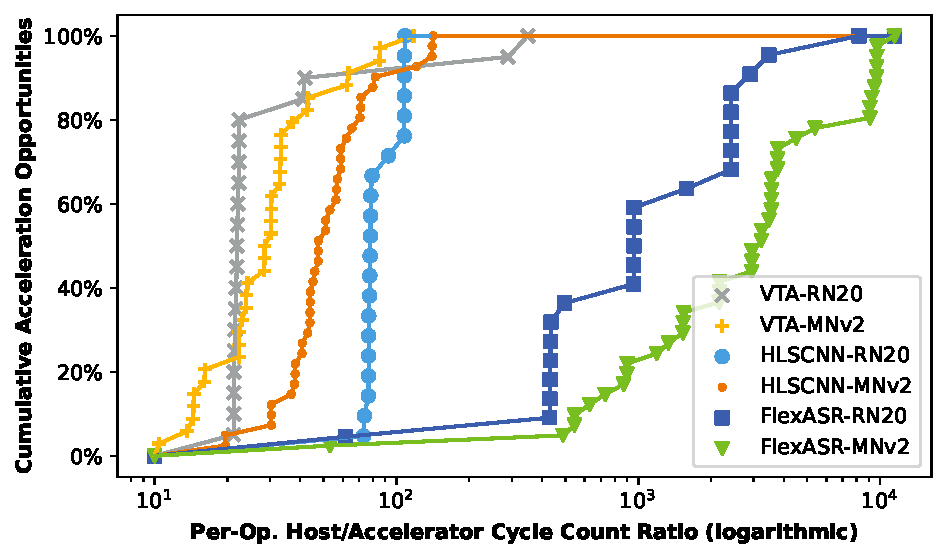
\includegraphics[width=.65\linewidth]{3la/Figures/performance.pdf}
  \caption{
\textbf{
Cumulative distribution of per-operator performance gains of all identified acceleration opportunities} in ResNet-20 (RN20) and MobileNet-V2 (MNv2) on the three accelerators.
%VTA, HLSCNN, and FlexASR.
Each point represents an operation offloaded from the host to the accelerator (as identified by flexible matching, Table~\ref{tab.compilation}).
The $x$-axis shows the host-to-accelerator cycle count ratio of each offloaded operation 
%(the bigger the better); 
and the $y$-axis shows the cumulative distribution of offloaded operations. Points and plots more to the right are better; e.g., coarse-grained operators, supported with higher parallelism in FlexASR, offer greater speedup compared to the fine-grained operators in VTA. %\sm{Change Accumulative in figure to Cumulative.}
%the y-axis accumulates toward all identified acceleration opportunities in an application.
%The measurement is done on 2000 random inputs from the CIFAR-10 dataset~\cite{cifar10}. \yl{The test inputs are not from CIFAR-10 dataset. It is just a random input with the same shape to the layer input in the applications}
}
  \label{fig.performance}
% \Description{}
\end{figure}

Fig.~\ref{fig.performance} shows the performance gains (ratio of host to accelerator cycles) of all identified acceleration opportunities in ResNet-20 and MobileNet-V2 when operations are offloaded from the host to VTA, HLSCNN, and FlexASR, respectively. 
%Figure~\ref{fig.performance} shows the cycle count ratios of all offloaded operations (from the host to the accelerator) in ResNet-20 and MobileNet-V2 when compiled to VTA, HLSCNN, and FlexASR.
%the three accelerators.
%Each point represents an operation offloaded from the host to the accelerator.
Overall, as expected, all offloads resulted in performance gains relative to the host; we also see that accelerators providing coarser-grained operators (e.g., FlexASR), supported with higher parallelism, achieve higher performance gain per operator compared to finer-grained accelerators like VTA. %\sslyu{Is this really something we should highlight? We don't discuss performance gains of coarse-grained vs fine-grained accelerators in the intro; our point is just that we gain performance compared to the host, which is what we're aiming for.}
%\aarti{
%Although the graph does not compare operator attributes, such as convolution strides, such per-operator performance evaluation can also provide additional insights on how these properties affect the performance of offloaded operators. 
%such as how the Conv2D operator performs under different stride attributes and \texttt{im2col} matrix dimensions.
%This could be useful in future work for performance optimization.
%} 
%\sslyu{Are we reporting any data to suggest that conclusion? We shouldn't say this if we don't. Otherwise, we could say that our methodology for getting the cycle counts could be used for assessing these issues.}
%We also find such per-operator performance evaluation insightful.
%Take VTA for example, {\TLA} provides a convenient way to analyze, within a real application, how the Conv2D operator performs under different convolution stride attributes and \texttt{im2col} matrix dimensions.
% From the operator-level performance analysis, we also see that VTA is not always good.
%We also found that the same Conv2D operator of VTA performs better when the convolution strides attributes align well with the \texttt{im2col} matrix dimensions---up to 10x difference in performance gain.
% \yl{VTA performs better stride attributes in the Conv2D are larger than 1. The reason is that larger strides would reduce the matrix size for matrix multiplications after doing im2col.}
%By measuring the performance of both running 2D Convolutions layers and running corresponding Dense matrix multiplications obtained from the \texttt{im2col} optimization, we found that VTA does not always gain performance from the optimization unless the strides attributes of the convolution layer keep the \texttt{im2col} matrix dimensions small enough. 
%(\yl{Not sure we should put the comparison between our codegen with original VTA codegen in here though. We are not using the original VTA codegen for Conv2D in our experiment. Also this comparison deviates a little from the other comparisons between acc. and host CPU.})
%(\mh{See numbers in the table and conv2d configurations of those layers}) 
%Under certain settings, the optimization brings up to 4x speed-up while in some other cases, it makes 2x worse performance compared with the baseline operator.
%Such per-operator performance evaluation provides insights on the identified acceleration opportunities in the full application compilation and is critical to more thorough performance optimization.
%It is critical to more thorough performance optimization.
%In this way, enabling per-operator performance evaluation would help accelerator users identify the right place to apply such optimizations.
%This study demonstrates that the {\TLA} methodology enables performance evaluation at the operator level, providing insights on how the identified acceleration opportunities perform in a full application.
%This is critical to future performance optimization.


\iffalse
\para{Proof-Based Formal Verification}
\label{sec:fv}
%%% there are differences, likely due to numerics, and we want to check that using abstract data types
%%% summrize: we can formally prove small scale op-level mappings

%%% As described earlier in Section~\ref{sec.method.verif}, verification of the full flow includes task VT2, which verifies equivalence of the ILA program fragment on the compiler side with that on the accelerator side. 
%%% This section describes a proof-of-concept study on the  Relay and FlexASR fragments for the temporal max-pooling application (see Appendix for the ILA code).

%%% In formally verifying the mappings, we use abstract data types to separate the effect of custom numerics.

The key challenges in formally verifying mappings between fragments that represent DL computations include:
\begin{inlinelist}
  \item handling nested loops, for both compiler side and accelerator side, that iterate through tensor elements, and
  \item relating tensor variables between the two sides which may employ various tiling mechanisms.%, and
%   \item handling custom numerics.
\end{inlinelist}
%
%%% Although the code of each ILA fragment is small, there are challenges due to:
%%% \begin{itemize}
%%%     \item multiple nested loops: 4 levels of nesting on Relay side, 3 on FlexASR side.
%%%     \item \emph{aligning} the nested loops for checking equivalence
%%%     \item mapping the input matrix to a special customized tiling provided by FlexASR~\cite{tambe20219}. \footnote{\hl{We ignore the FlexASR numerics accuracy in this study.}}
%%% \end{itemize} 
%
As a proof-of-concept study, we considered the Relay and FlexASR fragments for the FlexASR MaxPool IR-accelerator mapping. These fragments both have 
3+ nested loops, and the relation between the two fragments must account for a special customized tiling provided by 
FlexASR~\cite{tambe20219}.
For this study, we considered %
equivalence of the fragments over %
fixed-sized tensors with symbolic data,\footnote{Formally modeling custom numerics is left to future work.} and implemented verification using two methods:
\begin{inlinelist}
  \item bounded model checking (BMC)~\cite{biere2003bounded}, and 
  \item program verification using constrained Horn clauses (CHCs)~\cite{komuravelli2016smt}. 
\end{inlinelist}
%
The BMC-based method unrolls all the loops in both fragments, which is straightforward but may fail to scale for large-sized tensors.
%
The CHC-based method is given a product program of the two fragments and uses \emph{relational} loop invariants, i.e., formulas that relate the two fragments at intermediate loop boundaries (details are beyond the scope of this paper). 
%
This avoids loop unrolling and can handle large tensors. 
Both methods use Z3~\cite{de2008z3} as the underlying SMT solver.

% In our case study, we provided invariants that capture the customized tiling of FlexASR for fixed-sized matrices. 
% (In future work, we will consider automatic inference of such loop invariants.) 

While ILAng directly supports BMC, we manually created CHCs for the CHC-based method.
%for a 2D MaxPool operation in FlexASR. 
We also supplied the relational invariants that capture the customized tiling of FlexASR.
%
In future work, we plan to automate CHC generation, which will allow formal verification of other IR-accelerator mappings used in this paper.
%
Table~\ref{tab.verif-formal} shows the results for this case study for various dimensions of the 2D input matrix (Column~1), with runtimes of the BMC-based and CHC-based verification methods in Columns~2 and~3, respectively. 
%
The BMC-based method was able to verify equivalence of mappings with small-sized matrices, but timed out (with a 3-hour time limit) on the $16 \times 64$ matrix that was used for simulation-based validation. % (based on the available accelerator testcases).
%
In contrast, the CHC-based method was faster than BMC and successfully verified mappings with larger matrices. These results are encouraging and demonstrate how the \TLA methodology enables formal verification of key steps in the compilation flow. 
\fi
%
% Our results for both methods are reported in Table~\ref{tab.verif-formal}, for verification runtime on input matrices of various dimensions.
%TODO: add interpretation

%\subsection{End-to-End Testing}
\subsection{Application-Level Validation Through Co-Simulation}
\label{sec.end-to-end}

%Having validated the IR-accelerator mappings, we 
%We next explore how the small numerical differences at the level of individual operators affect the results of evaluating full applications.
%One main goal of the {\TLA} methodology is to
  %allows us to 
  %explore this through 
We performed application-level co-simulation
  %namely 
  by using the
  ILAng-generated simulators for accelerator computations
  and the host CPU for the rest of the computation.
%want to check if minor deviations at the single operation level will influence application-level behavior.
%
%Therefore, we performed application-level co-simulation on several applications which offload various computations to FlexASR and HLSCNN, the two accelerators that utilize custom numerics. (By co-simulation we mean simulating the software running on the host processor along with the operations off-loaded on the accelerator using the ILA simulator.)
%
%Specifically, we examined models that we were able to train and deploy on \hl{all of the devices (SM: unclear)} supported in our prototype:
We considered three applications,
  which between them provide opportunities to use
  each of the three accelerators: %,
  %as well as even combinations of them:
\begin{inlinelist}
  \item LSTM-WLM, where we accelerate linear layer and LSTM operations on FlexASR;
  \item ResNet-20, where we accelerate convolutions on HLSCNN and linear layers on FlexASR; and
  \item MobileNet-V2, where we accelerate convolutions and linear layers as in ResNet-20 and additionally accelerate both these operations on VTA (due to the \texttt{im2col} rewrites).
\end{inlinelist}
In ResNet-20 and MobileNet-V2,
  we were able to
  \emph{explore using HLSCNN and FlexASR together and separately}, simply by varying which 
  %IR-accelerator rewrites 
  {\mapping}s
  we included in flexible matching.

%Each of the three accelerators considered is used in some application, and even combinations of these accelerators are used in individual applications:
%\begin{inlinelist}
  %\item LSTM-WLM, whose linear layer and LSTM operations are supported by FlexASR;
  %\item \hl{ResMLP, whose linear layers are also supported by VTA}; and
  %\item ResNet-20 and MobileNet-V2, whose convolutions are supported by HLSCNN and whose linear layers are also supported by FlexASR, \emph{allowing us to explore using the accelerators together and separately}, simply by varying which IR-accelerator rewrites we include in the flexible matching step.
%\end{inlinelist}
%LSTM-WLM, which offload to FlexASR the LSTM layer and linear layer operations, respectively.
%
%We also considered MobileNet and ResNet, which both offload 2D convolution and linear layer operations to HLSCNN and FlexASR, respectively.
%
%(We compiled to two target accelerators by including the IR-accelerator rewrite rules for both accelerators.)
%
% As a sanity check \hl{(Was it a sanity check? It seems like an interesting case in its own right. -- Safety net in case we don't have a fully-matched VTA e2e in time so that we can drop it.)}, we also evaluated a quantized MobileNet on VTA, comparing application results under \hl{integer numerics, which have no rounding error}.


% Although the IR-accelerator mappings simulation shows acceptable relative errors, we don't know the mapping errors on a specific trained model or how these errors will accumulate across the layers and more importantly, how the numerical difference of the outputs will hurt the application-level results, such as the inference accuracy. Therefore, it is important to perform an application-level co-simulation to measure the correctness of the program running on the heterogeneous platform. This can be done by the compilation flow of the \TLA methodology which generates instructions sequences of the accelerator calls to run on the ILAng-generated software models.
% We pick the applications shown in the Table~\ref{tab.verif-sim} from the \AppNum compilation examples in Table~\ref{tab.compilation} to perform an application-level co-simulation. 
% These selected applications are relatively time-efficient for training and simulation, and some of them can utilize more than one accelerators for computation.


We trained and validated the LSTM-WLM model using the WikiText-2 dataset~\cite{merity2016pointer}.
%
The image classification models (MobileNet-V2 and ResNet-20) were trained and validated using the CIFAR-10 dataset~\cite{cifar10}.
We additionally trained and validated a MobileNet-V2 model optimized for ImageNet using the ImageNet dataset~\cite{deng2009imagenet}.

Table~\ref{tab.verif-sim} shows the application-level co-simulation results.
% Our quantization approach: Uniform quantization (calculated based on min and max value),
% we compute the scaling factor on the fly:
% we check the min and max values at run time
% and we compute the floating point reference value at run time to get a scaling factor for requantization
% Why is this morally defensible?
% Because in principle, we can get the scaling factor through a calibration run. We didn't bother doing that to simplify engineering tasks for ourselves. This may affect the results, but not in a huge way because, at the end of the day, this is not a paper about quantization
% \cite{jacob2017quantization}
%
%Columns~1 and~2 describe the application and the target processing platform under evaluation, respectively.
%
%We provide a reference result (perplexity for the text-generation task and inference accuracy for vision tasks) in Column~3 by running the application on the host processor, i.e., not offloading to accelerators.
%
%The application-level co-simulation 
%The validation result using original accelerator designs, labeled ``Original Result,'' is provided in Column~4.
%
%For cases where the ``Original Result'' was significantly poorer than the reference result, we reported it to the accelerator developers for their further investigation. 
%When they provided an accelerator design modification to address this, we provide an updated result, using this modified accelerator, in Column~5. 
%
%The average simulation time is reported in Column~6.
%
For LSTM-WLM,
  the application-level results using the accelerators
  did not differ greatly
  from the reference results.
In the case of FlexASR,
  this was the \textit{first time}
  it had been run end-to-end on a full application---%
  this provided validation for its AdaptivFloat data type.
For VTA on MobileNet-V2,
  there was a small decrease in accuracy
  that may be attributed
  to quantization error.%
\footnote{We apply a form of uniform quantization~\cite{jacob2017quantization},
  which involves scaling the results
  based on the floating point reference.}
%Typical implementations
  %involve pre-computing a scaling factor
  %using a floating point calibration run
  %on a representative dataset.
%To simplify our runtime,
  %our implementation
  %dynamically computes the scaling factor
  %by performing the floating point computation
  %on the current input
  %rather than using a calibration run.
%This approach is very inefficient
  %and may have different results 
  %compared to fixing a single scaling factor,
  %but it is presented only as a proof of concept,
  %since quantization is not the focus of this work.}

% I don't think we need this for dissertation.
%
% \input{Floats/tab-verif-e2e-combine.tex}

\begin{table*}
  \caption{
  \textbf{Application-level co-simulation results.}
  % Each validation evaluated 2000 data points (images for vision tasks and sentences for the text-generation task) evenly sampled from the corresponding dataset.
  In each test, we evaluated 2000 CIFAR-10 images (for vision tasks) or 100 WikiText-2 sentences (for text generation) that were evenly sampled from the corresponding dataset.
  % The reference accuracy is collected by running application inference on the host machine (x86). (Over 2000 evenly sampled data from the dataset.)
  % The initial and final accuracy are from the simulation on the heterogeneous platform enabled by \TLA with accelerator backends listed in the second column.
  The reference results were obtained by running tasks in the original frameworks (MxNet for ResNet-20, PyTorch for the rest).
  The {results without numerical tuning} are %measured using 
  for the initial accelerator designs, modeled in ILA.
  The {result with numerical tuning}, where provided, were obtained by updating the ILA specifications
  according to %to correspond to 
  design revisions suggested by the accelerator developers.
  We measured the accuracy for image classification tasks (ResNet-20, MobileNet-V2) and perplexity for text generation (LSTM-WLM).}
  % As LSTM-WLM is a text generation model, we report the perplexity of the generated text rather than classification accuracy.
  % \hl{(Please check):} Q-MobileNet is the result of applying an 8-bit quantization~\cite{jacob2017quantization} to MobileNet V2 after flexible matching, turning all matrix multiplications into quantized matrix multiplications via a pass in Relay.
  \label{tab.verif-sim}
  \centering
  \begin{small}
  \begin{tabular}{|l|c|c|c|c|r|}
  \hline
  % \multicolumn{1}{|c|}{Application} &
  %   \multicolumn{1}{c|}{Processing Platform} &
  %   \multicolumn{1}{c|}{Reference Result$^\ast$} &
  %   \multicolumn{1}{c|}{{Result without Numerical Tuning}} &
  %   \multicolumn{1}{c|}{{Result with Numerical Tuning}} &
  %   \multicolumn{1}{c|}{Avg. Sim. Time$^\dagger$} \\
  %   \hline \hline
      \multicolumn{1}{|c|}{\multirow{2}{*}{Application}} &
      \multirow{2}{*}{Processing Platform} &
      \multirow{2}{*}{Reference Result$^\ast$} &
      {Result without} &
      {Result with} &
      \multicolumn{1}{c|}{\multirow{2}{*}{Avg. Sim. Time$^\dagger$}} \\
    \multicolumn{1}{|c|}{} &
       &
       &
      {Numerical Tuning} &
      {Numerical Tuning} &
      \multicolumn{1}{c|}{} \\ 
    \hline \hline

  LSTM-WLM & 
    FlexASR & 
    122.15 & 
    121.97 & 
    N/A &
    22.4s \\
    \hline

%   ResMLP  & 
%     VTA & 
%     64.9\% & 
%     62.2\% & 
%     \hl{?} & 
%     56min 41s \\
%     \hline

  ResNet-20 & 
    FlexASR &
    91.55\% &
    91.50\% &
    N/A &
    11.6s \\
    
   &
    HLSCNN &
    91.55\% &
    \cellcolor[HTML]{E9CECE}29.75\% &
    \cellcolor[HTML]{DDEFDE}92.10\% &
    7min 3s \\
    
   &
    FlexASR \& HLSCNN & 
    91.55\% & 
    \cellcolor[HTML]{E9CECE}29.15\% & 
    \cellcolor[HTML]{DDEFDE}91.85\% & 
    7min 6s \\ 
    \hline

  MobileNet-V2 &
    VTA &
    92.40\% &
    89.40\% &
    N/A &
    20min 15s \\
  
   &
    FlexASR &
    92.40\% &
    92.30\% &
    N/A &
    18.1s \\

   & 
    HLSCNN & 
    92.40\% & 
    \cellcolor[HTML]{E9CECE}10.35\% & 
    \cellcolor[HTML]{DDEFDE}91.50\% & 
    20min 33s \\
    
   & 
    FlexASR \& HLSCNN & 
    92.40\% & 
    \cellcolor[HTML]{E9CECE}10.35\% & 
    \cellcolor[HTML]{DDEFDE}91.20\% & 
    21min 01s \\

  % Q-MobileNet-V2 & VTA & 91.80\% & \hl{10.80\%} & N/A & 43min 13s \\

    \hline
  \end{tabular}
  \end{small}
  \begin{tablenotes}
    \item $\ast$ The reference result does not represent the best achievable accuracy/perplexity of the model on the given dataset. This table is intended for comparing the application-level results on different processing platforms.
    \item $\dagger$ Average simulation time of running one data point (e.g., an image or a sentence) on an AMD EPYC-7532 core.
    % \item $\ddagger$ R.S.O. = issue reported; case still open.
  \end{tablenotes}
\end{table*}

%\input{Floats/tab-verif-e2e-imagenet}

However, the initial results for ResNet-20 and MobileNet-V2
  (both CIFAR-10 and ImageNet)
  using HLSCNN
  revealed a large loss in accuracy, 
  {as shown in Column~4 ``Results without Numerics Tuning'' in Table~\ref{tab.verif-sim}}.
%We were able to determine the root cause through subsequent experimentation:
We noticed that the linear layers 
  accelerated by FlexASR 
  did not impact the final accuracy,
  suggesting the issue stemmed from HLSCNN
  (for which this was also the first time it was run in an end-to-end application).
We then instrumented
  our {\TLA} prototype 
  %BYOC runtime 
  to record additional information
  for each accelerator invocation,
  such as input and output ranges.
%With this information,
This helped 
  the accelerator developers
  %were able to 
  determine that the loss of accuracy
  was due to a lack of dynamic range in the data type:
  weight data values 
  in HLSCNN's 2D convolutional layers
  were heavily quantized
  due to the narrow value range
  of their 8-bit fixed point representation.
%After we updated the ILA specification (an easier task than updating an RTL implementation) to use a 16-bit fixed point data type for weights with an adjusted binary point position (no longer using any 8-bit values)\mh{Do we need to explicitly say how much work was done?}, the applications recovered their accuracy.
After we updated the ILA specification (a much easier task than modifying the RTL implementation) based on the developers' suggestion to expand the fixed point representation to 16 bits and adjust the binary points in inputs' and accumulators' fixed point data types, the %full application 
accuracy recovered.
{This is shown in Column~5 ``Results with Numerics Tuning'' in Table~\ref{tab.verif-sim}.}
This case study readily demonstrates
  %thus also emphasizing
  how the {\TLA} methodology
  \textit{facilitates debugging and improving accelerator designs
  with rapid turnaround.}

\iffalse
{
Table~\ref{tab.verif-sim-imagenet} extend the application-level co-simulation experiment for offloading MobileNet-V2 application to the three target accelerators using the ImageNet dataset~\cite{deng2009imagenet}.
Comparing it with Table~\ref{tab.verif-sim}, we can see that there is an significant accuracy drop, i.e., from 10.35\% down to 0.10\%, for the results without numerical tuning when HLSCNN is involved.
This marked decrease in accuracy is due to the augmentation in the number of classification classes—increasing from 10 in the CIFAR-10 dataset to 1000 in the ImageNet dataset—as well as the increase in input image resolution—from 1x3x32x32 pixels in CIFAR-10 to 1x3x224x224 pixels in ImageNet. 
This end-to-end application-level co-simulation again help our accelerator developers to identify the lack of dynamic range of the original 8-bit fixed point representation, and the precision mismatch resulting from the binary points configuration in input's, accumulators' and outputs' fixed point data types.
The accuracy is recovered after similar numerical tuning is applied.
}
\fi

%We reported the original validation accuracy of ResNet-20, 
% 29.15\% accuracy, 
%which was much worse from the 91.55\% reference result, to the accelerator developers. 
%
%We also provided statistics for each accelerator invocation (e.g., error accumulation, input and output ranges, etc.), gathered by our compiler prototype and ILA simulators.
%
%With the information, the accelerator developers were able to identify the root cause: weight data values in HLSCNN's 2D convolutional layers were heavily quantized by its 8-bit fixed point data type due to a narrower value range.
%
%After updating the design by expanding the original 8-bit representation to 16 bits, the application-level result matched up to the reference result.
%
%The same tuning approach also resulted in improved accuracy for MobileNet-V2.


% In the ResNet-20 case study, we only achieve 29.15\% of inference accuracy initially with computation using the original configurations of custom numerical representation on the accelerators. This inference accuracy is far from the 91.55\% reference accuracy running on the host processor. To investigate the issue, we extracted the intermediate results of each layers offloaded to the accelerators and compared them to the reference results of the same layer to investigate how errors are accumulated across different offloading layers. In the per-layer analysis, we found out that several 2-D convolutional layers on HLSCNN shows greater relative errors, which is due to a significant narrower range of the weight data values that are heavily quantized by the 8-bit fixed point representation. As a result, we expand the original 8-bit representation into 16 bits, providing a finer-grain quantization to fit the data, and the final inference accuracy is improved to 91.85\%, very close to the reference accuracy. Similar tuning on the accelerator implementation also happens in our MobileNet case study, in which the initial accuracy is only 10.35\% compared with a 92.40\% reference. However, only expanding the bitwidth for weight data is not enough for this application. We also reassigned the bits in the 16-bit fixed-point representation for the activations in HLSCNN to better match its data distribution in the application. The final accuracy is improved to 91.20\% for MobileNet-V2 after the further tuning of the accelerator. 
% \hl{Discussion on LSTM and qnn-mobilenet.} 

The overall results in Table~\ref{tab.verif-sim} reaffirm the need for application-level validation, especially for accelerators utilizing custom numerics.
%
%However, without an end-to-end compilation flow, such application-level validation is prohibitively difficult for new accelerators.
%
%Our experiments demonstrate how \TLA provides systematic and largely automatic compilation-results validation at the application level and also show its usefulness in software/hardware co-design.
%
%Specifically, due to 
Thanks to formal ILA models, \TLA provides quick design space exploration and numerics tuning without hardware engineering overhead %(e.g., deploying to FPGA) 
in each design iteration.
%
%A repetitive
%Other than the accelerator ILAs and the compiler IR--ILA patterns (a one-time-per-accelerator effort independent of the application), integration into the compiler required only a small number of Glenside rewrite rules and a small code generator mapping matched patterns to ILA instructions.
%
Further, it provides handy debugging information and efficient simulation---%
%
for FlexASR, the ILA simulator yields a 30$\times$ speedup on average compared to RTL simulation.
%using a 
% state-of-the-art 
%commercial Verilog simulator.
%Synopsys VCS~\cite{vcs}.)

% These case studies shows our \TLA's great advantage in software/hardware co-design. The portability of \TLA enabling us to automatically support application level co-simulation on a variety of applications by using ILA as a formal software/hardware interface. By contrast, similar application-level co-simulation with accelerator APIs would require significant amount of human efforts to map each DSL application to the accelerator calls. 
% This co-simulation could provide valuable feedback for software/hardware co-design. For example, accelerators' numerical representation settings may need to be tuned to adapt to different applications to provide an reasonable accuracy with its power-performance benefits, as it is shown in our case studies. Moreover, running application-level simulation would help discover issues in the early-stage hardware design, which could possibly be hidden in the traditional per-instruction/layer validation method. On the other hand, software designers could tweak their applications based on the feedback of the results using the accelerators, such as running accelerator specific quantization-aware training or tuning the parameters in the models, to improve the target metrics.

% In the meantime, the automatically-generated software models from the hardware accelerator ILA models enable efficient co-simulation for the early stage software-hardeware co-design. As a comparison, the measured time of the generated FlexASR ILA simulation is about 10$\times$ faster than its High-level Synthesis (HLS) model simulation (using Catapult HLS \cite{catapult}) and has on average 30$\times$ speed-up against the RTL simulation (using Synopsys VCS \cite{vcs}). 
% The total simulation time of the case studies shown in the table can be easily reduced down to a few hours with a distributed computing setup. For example, in the ResNet-20 experiment, the simulation time is reduced down to 4 hours using 125 same cpu cores. 
% Moreover, the generated ILA simulation models can serve as functional model for early-stage design and validation when the HLS or RTL models of the accelerators are not ready.
% this cannot be done in previous approaches, due to the lack of an interface that is abstract while capturing formal semantics
% re-iterate the RTL simulation is slow and limits early stage codesign

%\hl{Gus:
%  We should add an asterisk
%  on VTA/Mobilenet
%  to say that we ran
%  a quantization pass
%  in order to be able to map
%  mobilenet to VTA.
%This is in lieu of
%  having a separate Q-Mobilenet
%  column
%  in the flexmatching table.}
\subsection{System Deployment and FPGA Emulation}
\label{sec.eval-fpga}

As an additional demonstration of {\TLA}, we explored its use in 
%To demonstrate that the {\TLA} flow also supports 
  compiling workloads
  to a real hardware platform.
  Specifically, 
  we used our prototype to compile workloads
  to an FPGA emulation of FlexASR.%
\footnote{We synthesized and placed-and-routed the FlexASR accelerator on a Xilinx Zynq ZCU102 FPGA, which consumed 86\% of the available LUT resources.
Due to the significant engineering overhead of FPGA emulation, FlexASR is the only accelerator we deployed on an FPGA.}
%We synthesized and placed-and-routed the FlexASR accelerator on a Xilinx Zynq ZCU102 FPGA, which consumed 86\% of the available LUT resources.%
%
%The approach was conceptually simple:
We configured our prototype to lower
 FlexASR ILA instructions
 to the corresponding MMIO commands for FlexASR, % (a trivial translation thanks to the one-to-one correspondence between the ILA instructions and MMIO commands),
 passing them to the FPGA using the Xilinx SDK~\cite{xsdk}.
%We utilized the Xilinx SDK~\cite{xsdk} to pass the accelerator instructions (MMIO commands) to the accelerator interface for invoking the supported operations.
%
%Specifically, 
Next, we compiled and executed synthetic workloads in which LSTM layers and linear layers were offloaded to the FlexASR accelerator.
The results matched those of the ILAng-generated simulator bit for bit, providing validation for %the software simulation of 
the custom numerics.
%\hl{AG: what is the punchline -- was this successful? how much effort?}
%With only light modifications to our previous FlexASR code generator, we were able to convert our simulated trials into executions on the FPGA.\mh{same as the previous comment: do we expand here on what to do specifically?}
%Although only a proof of concept, this case study demonstrates that the {\TLA} methodology can be potentially extended to a complete compilation flow. 
This is a proof of concept for utilizing the {\TLA} methodology for an actual deployment, above and beyond simulation-based testing.
  %and not just end-to-end testing.
  %provides a principled and extensible means
  %of compiling applications to new accelerators 
  %\hl{AG: seems meh}.
%This case study demonstrates the applicability of \TLA in actual system deployment on a commodity hardware platform.
%
%Further, it shows that in the absence of compilation-results validation enabled by the \TLA methodology, the need for a fully functional RTL model and the significant engineering overhead indeed limit early-stage software/hardware co-design.



% \subsection{Extensibility}
% How hard to add a new accelerator support.


\part{Compilation to FPGAs}

\chapter{Conclusion}
\chapter{Broader Thoughts}

Though this dissertation
  is meant to seem like a polished and cohesive
  story,
  the actual path to a PhD is much
  more winding and twisted.
In this section, I want to chronicle
  the higher level thoughts,
  ideas, and inspirations
  underlying the projects in my dissertation
  (and some projects that didn't make it in).


\hl{hannah's thought re: generating hardware from software vs generating software from hardware as we suggest here } 

\clearpage
\addcontentsline{toc}{chapter}{Bibliography}
\singlespacing
\bibliographystyle{plain}
\bibliography{references}

\end{document}